% vim:fmr=[[[,]]]:fdm=marker
% by Jerry Fleming <jerryfleming2006@gmail.com>
% on 2013-03-25.
% All rights reserved.
% coding: utf8

% preamble [[[

\documentclass[openany,notitlepage]{book}

% [[[ packages
\usepackage{makeidx}
\usepackage{CJKutf8}
%\usepackage[utf8]{inputenc}
\usepackage{CJKnumb}
\usepackage{CJKpunct}
\usepackage{nameref}
\usepackage{color}
\usepackage{float} % for [H], must comes before hyperref
\usepackage{hyperref}
\usepackage{fancyhdr}
\usepackage{fancybox}
\usepackage{titlesec}
\usepackage{titletoc}
\usepackage[titles]{tocloft} % for List of Notes
\usepackage[chapter]{tocbibind} % to include to[clf] in toc
\usepackage{appendix}
\usepackage{multicol} % for \theindex
\usepackage{fullpage}
\usepackage{graphicx}
\usepackage{eso-pic} % for fullpage covers
\usepackage{tikz}
\usepackage{pifont} % for \ding
\usepackage{datetime} % to renew \today
\usepackage{indentfirst}
\usepackage{keystroke}
% packages ]]]

\makeindex

% pdf styles [[[
\hypersetup{
    bookmarksopen=true,
    backref=true,
    unicode=true, % non-Latin characters in Acrobats bookmarks
    pdftoolbar=true, % show Acrobat's toolbar?
    pdfmenubar=true, % show Acrobat's menu?
    pdffitwindow=false, % page fit to window when opened
    pdftitle={Bash 参考手册}, % title
    pdfauthor={邵加超 Jerry Fleming}, % author
    pdfsubject={company}, % subject of the document
    pdfnewwindow=true, % links in new window
    pdfkeywords={Bash,邵加超,Jerry Fleming,参考手册,中文文档,Linux,命令}, % list of keywords
    colorlinks=true, % false: boxed links; true: colored links
    linkcolor=red, % color of internal links
    citecolor=green, % color of links to bibliography
    filecolor=magenta, % color of file links
    urlcolor=cyan, % color of external links
    plainpages=true % use formatted page number
}
% this is to fix a bug in hyperref, which hornors linktocpage option as a boolean wrongly
\makeatletter
\let\Hy@linktoc\Hy@linktoc@all
\makeatother
% pdf styles ]]]

% [[[ colors
\definecolor{row}{rgb}{.9,.9,.9}
\definecolor{skyblue}{RGB}{97,203,222}
% colors ]]]

% [[[ headers
\addtolength{\voffset}{-.6in}
\setlength{\headsep}{10pt}
\setlength{\footskip}{45pt}
\setlength{\headheight}{40pt}
\renewcommand{\headrulewidth}{.2pt}
\renewcommand{\footrulewidth}{.2pt}
\renewcommand{\footruleskip}{2pt}
\setlength{\arrayrulewidth}{.2pt}
\fancypagestyle{myfancy}{
    \fancyhead[C]{
        \setlength{\unitlength}{1in}
        \begin{picture}(0,0)
            \color[gray]{.95}
            \put(-1,-5){\makebox(2, 2){\rotatebox{45}{\scalebox{10}{\Large\CJKfamily{gkai}{草稿}}}}}
        \end{picture}
    }
    \fancyhead[RO,LE]{\leftmark}
    \fancyhead[RE,LO]{\rightmark}
    \fancyfoot[LE]{\textcolor{gray}{\raisebox{-.35\height}{
\includegraphics{geofuture_h.png}} BASH 中文文档}}
    \fancyfoot[RO]{\textcolor{gray}{BASH 中文文档 \raisebox{-.35\height}{
\includegraphics{geofuture_h.png}}}}
    \fancyfoot[C]{\nameref{content}}
    \fancyfoot[RE,LO]{
        \begin{picture}(30,5)
            \color{skyblue}
            \put(0,0){\scalebox{2.5}[1]{\circle*{15}}}
            \color{black}
            \put(0,0){\makebox(0,0){\textit{p\thepage}}}
        \end{picture}
    }
    \renewcommand{\headrule}{
        \begin{picture}(430,10)(10,-5)
            \color{skyblue}
            \put(0,0){\circle*{10}}
            \multiput(13,0)(10,0){49}{\circle*{6}}
        \end{picture}
    }
    \renewcommand{\footrule}{
        \begin{picture}(430,10)(10,0)
            \color{skyblue}
            \put(492,0){\circle*{10}}
            \multiput(0,0)(10,0){49}{\circle*{6}}
        \end{picture}
        \vskip 3pt
    }

}
\fancypagestyle{myplain}{
    \fancyhead[C]{
        \setlength{\unitlength}{1in}
        \begin{picture}(0,0)
            \color[gray]{.95}
            \put(-1,-5){\makebox(2, 2){\rotatebox{45}{\scalebox{10}{\Large\CJKfamily{gkai}{草稿}}}}}
        \end{picture}
    }

    \fancyhead[RO,LE]{\leftmark}
    \fancyhead[RE,LO]{\rightmark}
    \fancyfoot[LE]{\textcolor{gray}{\raisebox{-.35\height}{
\includegraphics{geofuture_h.png}} BASH 中文文档}}
    \fancyfoot[RO]{\textcolor{gray}{BASH 中文文档 \raisebox{-.35\height}{
\includegraphics{geofuture_h.png}}}}
    \fancyfoot[C]{}
    \fancyfoot[RE,LO]{
        \begin{picture}(30,5)
            \color{skyblue}
            \put(0,0){\scalebox{2.5}[1]{\circle*{15}}}
            \color{black}
            \put(0,0){\makebox(0,0){\textit{p\thepage}}}
        \end{picture}
    }
    \renewcommand{\headrule}{
        \begin{picture}(430,10)(10,-5)
            \color{skyblue}
            \put(0,0){\circle*{10}}
            \multiput(13,0)(10,0){49}{\circle*{6}}
        \end{picture}
    }
    \renewcommand{\footrule}{
        \begin{picture}(430,10)(10,0)
            \color{skyblue}
            \put(492,0){\circle*{10}}
            \multiput(0,0)(10,0){49}{\circle*{6}}
        \end{picture}
        \vskip 3pt
    }

}
\fancypagestyle{plain}{
    \fancyhead[C]{
        \setlength{\unitlength}{1in}
        \begin{picture}(0,0)
            \color[gray]{.95}
            \put(-1,-5){\makebox(2, 2){\rotatebox{45}{\scalebox{10}{\Large\CJKfamily{gkai}{草稿}}}}}
        \end{picture}
    }
    \fancyhead[RO,LE]{\leftmark}
    \fancyhead[RE,LO]{\rightmark}
    \fancyfoot[LE]{\textcolor{gray}{\raisebox{-.35\height}{
\includegraphics{geofuture_h.png}} BASH 中文文档}}
    \fancyfoot[RO]{\textcolor{gray}{BASH 中文文档 \raisebox{-.35\height}{
\includegraphics{geofuture_h.png}}}}
    \fancyfoot[C]{}
    \fancyfoot[RE,LO]{
        \begin{picture}(30,5)
            \color{skyblue}
            \put(0,0){\scalebox{2.5}[1]{\circle*{15}}}
            \color{black}
            \put(0,0){\makebox(0,0){\textit{p\thepage}}}
        \end{picture}
    }
    \renewcommand{\headrule}{
        \begin{picture}(430,10)(10,-5)
            \color{skyblue}
            \put(0,0){\circle*{10}}
            \multiput(13,0)(10,0){49}{\circle*{6}}
        \end{picture}
    }
    \renewcommand{\footrule}{
        \begin{picture}(430,10)(10,0)
            \color{skyblue}
            \put(492,0){\circle*{10}}
            \multiput(0,0)(10,0){49}{\circle*{6}}
        \end{picture}
        \vskip 3pt
    }

}
% headers ]]]

% [[[ sections and titles
\renewcommand{\contentsname}{目录}
\renewcommand{\indexname}{索引}
\renewcommand{\appendixname}{附录}
\renewcommand{\appendixpagename}{\appendixname}
\renewcommand\appendixtocname{\appendixname}
\titleformat{\chapter}{\Huge\center}{第\CJKnumber{\thechapter}章}{20pt}{}[\rule{.6\textwidth}{4pt}]
\pagestyle{fancy}
\renewcommand{\theparagraph}{\Alph{paragraph}}
\titleformat{\paragraph}{\large}{\raisebox{-2pt}{\rule{10pt}{12pt}} \theparagraph .}{10pt}{}[\vspace{\parskip}]
\setlength{\cftparanumwidth}{15pt}
\newcommand{\xquad}{\hspace{1em plus.4em minus.4em}}
%\titlecontents*{paragraph}[.3\textwidth]{\small}{\P\thecontentslabel\hspace{4pt}}{}{,\hspace{4pt}\textit{p\thecontentspage}}[][\xquad ---\xquad ][.]
\setcounter{secnumdepth}{5} % include \paragraph as well
\setcounter{tocdepth}{5} % include \paragraph as well
\renewcommand{\cftchappresnum}{第}
\renewcommand{\cftchapaftersnum}{章}
\renewcommand{\cftsecpresnum}{\S}
\setlength{\cftsecnumwidth}{3.1em}
\renewcommand{\cftsubsecpresnum}{\S}
\renewcommand{\cftsubsubsecpresnum}{\S}
\setlength{\cftchapnumwidth}{40pt}
\titlelabel{\S\,\thetitle\quad}
\renewcommand{\cftaftertoctitle}{\vspace{2pt}\rule{.6\textwidth}{4pt}}
\renewcommand{\dateseparator}{-}
\renewcommand{\today}{\the\year \dateseparator \twodigit\month \dateseparator \twodigit\day}
\setlength{\parindent}{2em}
% sections and titles ]]]

% faq [[[
\newlistof{faqs}{faq}{常见问题}
\newcommand{\question}[1]{%
    \ifnum\value{faqs} > 0
        \label{faq:\thefaqs}%
        \addcontentsline{faq}{faqs}{\protect\numberline{\thefaqs}#1}%
    \fi
    \noindent\begin{tikzpicture}[remember picture] \node [xshift=1cm,yshift=1cm] [fill=red!20,rounded corners] {
    \raisebox{-1.1em}{%
        {\Huge\CJKfamily{gkai}{\color{red}问}}%
        \raisebox{1em}{\color{red}\large\thefaqs .}%
    }
    \begin{minipage}[t]{.9\textwidth}#1\end{minipage}%
    };
    \end{tikzpicture}%
    \par
    \refstepcounter{faqs}
}
\newenvironment{answer}[1]{%
    %\par\noindent\hangindent=3em \hangafter=1
    %\leavevmode{%
    %    \hbox{\raisebox{-.7\height}[0pt][0pt]{\CJKfamily{gkai}{\Huge\color{red}答}}}}
    \par#1
}
{\vskip 5pt}
% faq ]]]

% misc [[[
% item label
\renewcommand{\thefootnote}{\textcolor{red}{[\arabic{footnote}]}}
\renewcommand{\descriptionlabel}[1]{\hspace{\labelsep}\thinlines\setlength{\fboxsep}{0pt}\fbox{\,\raisebox{-1ex}{\textcolor{white}{\rule{1px}{3.5ex}}}\textbf{#1}\,}\hspace{10pt}}
\renewcommand{\labelitemi}{\ding{43}}
\renewcommand{\labelenumi}{
    \begin{picture}(10,10)(-5,-2)
        \color{gray}
        \put(0,0){\circle*{15}}
        \color{white}
        \put(0,0){\makebox(0,0){\textit{\theenumi}}}
    \end{picture}
}
% inline pic
\newcommand{\inlinepic}[1]{%
    \lower -.5ex\hbox{%
        \raisebox{.5\totalheight}{\includegraphics{#1}}
    }
}
\makeatletter
\def\flushboth{%
  \let\\\@normalcr
  \@rightskip\z@skip \rightskip\@rightskip
  \leftskip\z@skip
  \parindent 2em\relax}
\makeatother
\renewcommand{\textasciitilde}{\path+~+}

% misc ]]]

% note [[[
\newcommand{\note}[3][info]{%
    \vskip 5pt
    \begin{tikzpicture}[remember picture] \node [xshift=1cm,yshift=1cm] [draw=red,thick,rounded corners] {
    \begin{minipage}{.9\textwidth}
    \raisebox{-5pt}{\includegraphics[width=20pt]{box_#1.jpg}} {\large\CJKfamily{gkai}{\color{red}#2}}
    \vskip 5pt
    #3
    \end{minipage}
    };
    \end{tikzpicture}
}
% note ]]]

% [[[ codeline
\newcommand{\codelinenum}[1]{\par\rule{.1\textwidth}{.3pt} \textit{p\pageref{codeline:#1}} \rule{.1\textwidth}{.3pt}\par\vskip 20pt}
\newcommand{\codelinetext}[1]{\par\noindent#1}
\makeatletter
\newcounter{codeline}
\newcommand{\codeline}[2]{
    \begin{center}
    \begin{tikzpicture}[remember picture] \node [xshift=1cm,yshift=1cm] [text width=.8\textwidth,fill=green!20,rounded corners] {
       \begin{minipage}{.97\textwidth}#1\end{minipage}
    };
    \ifnum\value{csts} > 0
        \label{codeline:\thecodeline}
        \protected@write\@auxout{}{%
            \string\@writefile{line}{\string\codelinetext{#1}}
            \string\@writefile{line}{\string\codelinenum{\thecodeline}}
        }%
    \fi
    \end{tikzpicture}
    \end{center}
    \refstepcounter{codeline}
}
\makeatother
% ]]]

% [[[ codelist
\newcommand{\listcstsname}{代码列表}
\newlistof{csts}{cst}{\listcstsname}
\newenvironment{codelist}[1]
{
    \ifnum\value{csts} > 0
        \label{cst:\thecsts}
        \addcontentsline{cst}{csts}{\protect\numberline{\thecsts}#1}
    \fi
    \begin{quotation}\noindent%
    \begin{tikzpicture}[remember picture] \node [xshift=1cm,yshift=1cm] [text width=.9\textwidth,fill=row] {
    \textcolor{red}{\ding{107} 代码清单 \thecsts :#1}
    };
    \end{tikzpicture}\par\noindent\tt{}%
}
{
    \par\noindent\normalfont%
    \begin{tikzpicture}[remember picture] \node [xshift=1cm,yshift=1cm] [text width=.9\textwidth,fill=row] {};
    \end{tikzpicture}%
    \end{quotation}
    \refstepcounter{csts}
}
\newcommand{\codeblock}[1]{\begin{center}\begin{minipage}{.7\textwidth}{\tt #1}\end{minipage}\end{center}}
\newcommand{\codeConstant}[1]{\textcolor[RGB]{0,205,0}{\texttt{#1}}}
\newcommand{\codeComment}[1]{\textcolor[RGB]{255,96,96}{\texttt{#1}}}
\newcommand{\codeIdentifier}[1]{\textcolor[RGB]{0,255,255}{\texttt{#1}}}
\newcommand{\codeSpecial}[1]{\textcolor[RGB]{255,20,147}{\texttt{#1}}}
\newcommand{\codeOperator}[1]{\textcolor[RGB]{128,128,255}{\texttt{#1}}}
\newcommand{\codePreProc}[1]{\textcolor[RGB]{205,0,205}{\texttt{#1}}}
\newcommand{\codeRepeat}[1]{\textcolor[RGB]{255,255,255}{\texttt{#1}}}
\newcommand{\codeStatement}[1]{\textcolor[RGB]{0,0,255}{\texttt{#1}}}
\newcommand{\codeType}[1]{\textcolor[RGB]{20,0,255}{\texttt{#1}}}
\newcommand{\codelnr}[1]{\textcolor[RGB]{165,42,42}{\scriptsize\texttt{#1}}}
% ]]]

% [[[ context commands
\newcommand{\mnemonic}[1]{\textcolor{gray}{{\scriptsize\tt 助记词: #1}}}
\newcommand{\code}[1]{\textcolor{blue}{{\tt #1}}}
\newcommand{\hl}[1]{{\sl #1}}
\newcommand{\hs}[1]{{\textcolor{violet}{#1}}}
% seperate the paragraph end from the rest of upper layer section
\newcommand{\stopparagraph}{\par\vspace{5pt}\noindent\raisebox{-2pt}{\rule{10pt}{12pt}} {\bf [分节结束]}\vspace{5pt}}
\newcommand{\tab}{\mbox{\ \ \ \ }}
% context commands ]]]

% [[[ refs and labels
% reference to subparts of \lebelsection will display the section title/label instead of the ones for various subparts
\def\currentlabeltitle{}
\def\currentlabelnum{}
\newcommand{\labelsection}[1]{\def\currentlabeltitle{#1}\section{#1}\def\currentlabelnum{\thesection}}
\newcommand{\labelsubsubsection}[1]{\def\currentlabeltitle{#1}\subsubsection{#1}\def\currentlabelnum{\thesubsubsection}}
\makeatletter
\def\ulabel#1{%
    \@bsphack
    \begingroup
    \protected@write\@auxout{}{%
        \string\newlabel{#1}{%
            {\currentlabelnum}%
            {\thepage}%
            {\currentlabeltitle\,\, \@currentlabelname}%
            {\@currentHref}{}%
        }%
    }%
    \endgroup
    \@esphack
}%
\makeatother
\newcommand{\fullref}[1]{\,\S\,\ref{#1}[\nameref{#1}], \textit{p\pageref{#1}}\,}
% ]]]

% preamble ]]]

\begin{document}
\begin{CJK}{UTF8}{song}

% front issues [[[
\frontmatter
\pagenumbering{alph}
\setcounter{page}{1}
\pagestyle{empty}

\begin{titlepage}
\AddToShipoutPicture*{\put(0,-43.4){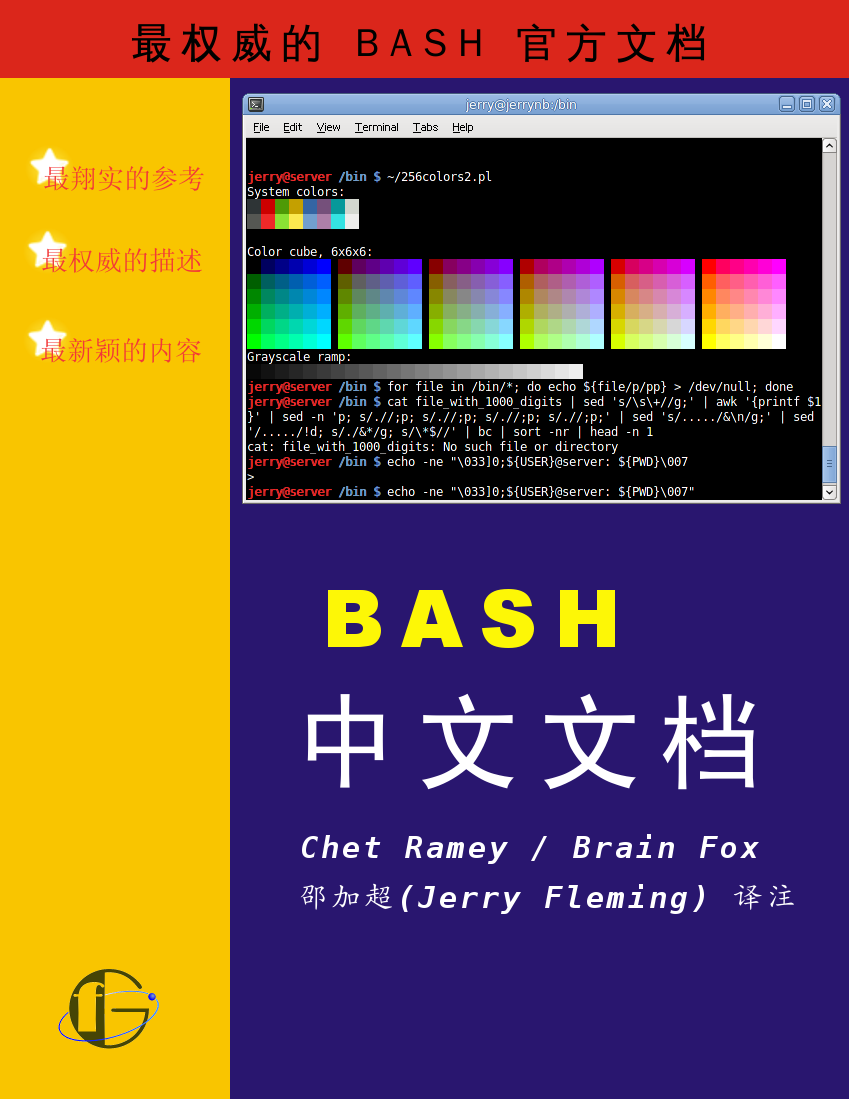
\includegraphics[width=\paperwidth,height=\paperheight]{frontcover.png}}}
\
\end{titlepage}

%\begin{titlepage}
\thispagestyle{empty}
\begin{center}\ \end{center}
\begin{center}
\scalebox{2}{\textcolor{red}{\Huge\CJKfamily{gkai}{BASH 中文文档}}}
\vskip 10pt
\rule{.7\textwidth}{4pt}
\vskip 30pt
{\Large Chet Ramey, Brian Fox}  {\Large\textsl{著}}

{\Large 邵加超(Jerry Fleming)}  {\Large\textsl{译注}}
\vskip 10pt
{\Large 最后更新于 \today}
\vfill

\includegraphics[width=100px]{geofuture.png}
\vskip 15pt
{\Large\code{Bash} 4.0 参考文档}\\
\vskip 5pt
\href{mailto:jerryfleming2006@gmail.com}{\Large jerryfleming2006@gmail.com}
\end{center}
%\end{titlepage}
\newpage
\begin{center}\ \end{center}
\par
\vskip 80pt
\begin{center}
{\Large 献给}\\
我的妻子和孩子们\\
感谢他们的谅解,使我有足够的业余时间翻译完这本书
\end{center}
\newpage


\pagenumbering{roman}
\setcounter{page}{1}
\pagestyle{myplain}

\renewcommand{\chaptermark}[1]{\markboth{#1}{}}
\renewcommand{\tocetcmark}[1]{\markboth{#1}{}}
\chapter{译者序}\label{test}

人们在学习新事物时往往急于看到它的全貌,而看到全貌时却又失之于细节。学习和使用 Bash 尤其如此。尽管它是 Linux 的首选 shell,但是因为它与我们所熟知的``高级语言''是如此不一致,以至于即使是从业多年的老程序员,写起 shell 程序来也会觉得力不从心。而 Bash 最权威的参考资料,即其程序作者所著的《Bash Reference Manual》,又因为语言的问题不能尽为中国程序员和 IT 从业人士所知悉。所以在很多时候,我们对刚刚崛起的 Linux 只能望洋兴叹。我正是试图改变这种现状才翻译这本书的。事实上,最初促使我翻译的动机并不是来自 Bash 本身,而是来自 \LaTeX{}。在学习 \LaTeX{} 多年以后,我很想做出一些东西来,于是就选择了翻译这本书,因为我使用 Bash 有七八年了,颇有一些心得。这些心得会以脚注或或者备注等形式体现出来。

为了准确的呈现原文的内容,本文在很多地方都做了特殊处理。首先是某些地方中文和英语的表达习惯不一样,为了使中文更具可读性,在不改变原意的情况下,我对原来的语句做了适当的调整。有些地方还加了脚注。原文是用 \code{texinfo} 来排版的;这便于在计算机上阅读,而排版并翻译成中文却有诸多不便。所以我对原稿的显示风格做了大量的改动,使得翻译出来的中文版更方便阅读和打印。此外,本书原文中有很多地方都对命令进行交叉引用,而命令又很多,只找到章节标题并不能很快的定位到想要查看的命令。所以在交叉引用命令时,我大都做一些改动,以方便读者。

每个页面的页脚中都中指向目录的链接;这样如果在电脑上阅读本书而不是打印,将会非常方便。\hl{1234567890} 是一个数字。\Return\ 是键盘上的一个键;有的键,例如 \keystroke{C-a} 需要和 \keystroke{Control} 等其它键一起输入。\code{abc} 是代码行中的一个或多个单词,可以在命令行中输入或写入到文件中。而 \mnemonic{Mnemonic, 助记词} 是用来帮助记忆命令或选项的;这些助记词大多数情况下都是来自它所解释对象的英文表达,有些时候则纯粹是为了记忆写臆造的。另外,本书中的交叉引用都是采用``章节号 标题 页码''的完整格式,例如\fullref{test}。

\codeblock{\textsl{\small{这是应该在命令行中输入的文本。}}}

\codeline{这段是命令格式的说明。其中的\hs{高亮字体}部分将在后面的详细讲解中用到。所有的命令格式都在附录中列出。}

\noindent\note[info]{你知道吗?}{这是和上下文相关的作息。}

\note[tip]{使用小窍门}{这是一些小窍门。}

\note[forbid]{注意事项}{这是一些典型的错误用法。}

\begin{codelist}{代码清单说明}%
{\scriptsize 这是一些可以直接使用的代码片段。它采用了 Vim 形式的高亮显示,并且加上了行号。}
\end{codelist}

\question{这是``常见问题''中的问题与答案。}

本书是在 Gentoo Linux 下的 TexLive 环境中使用 Vim 编辑的。成书以后,用 CTexLive2008 最后编译了一次,因为那里的字体好看~(感谢 CTexLive2008 的制作者们)。

本书尚未译完时就有很多读者朋友要求印刷,因为在电脑上看书很伤眼睛。我也正在考虑这件事。如果您愿意购买纸质版本,请尽早\href{mailto:jerryfleming2006@gmail.com}{发邮件}和我联系。
\vskip 30pt

\hfill\begin{minipage}{.3\textwidth}
\begin{center}
译者\\
2009年秋
\end{center}
\end{minipage}

\begin{center}
\tableofcontents
%\addcontentsline{toc}{chapter}{\contentsname}
\label{content}
\chapter{\listcstsname}
\makeatletter
\@starttoc{cst}
\makeatother
\end{center}

\mainmatter
\pagenumbering{arabic}
\setcounter{page}{1}
\pagestyle{myfancy} % this dummy line is required by \chaptermark and \sectionmark

% front issues ]]]

\renewcommand{\chaptermark}[1]{\markboth{第\CJKnumber{\thechapter}章 \MakeUppercase{#1}}{}}
\renewcommand{\sectionmark}[1]{\markright{\S\,\thesection\ \MakeUppercase{#1}}}

\chapter{总体介绍} % [[[
\section{什么是 Bash?} % [[[
Bash 是一个用于 GNU\footnote{即 Linux。} 操作系统的 shell,也就是命令解释器。这个名字是``Borune-Again SHell''\footnote{意为``波恩 shell 的再生''。}\index{shell!波恩 shell}的缩略词,意在调侃斯蒂芬\textbullet 波恩;他写的 \code{sh} 是目前 Unix 命令行解释器的前身,最初出现于被贝尔实验室研究用 Unix 的第七版。

Bash 整体上保持与 \code{sh} 兼容,并且从科恩 shell \code{ksh}\index{shell!ksh} 和 C shell \code{csh}\index{shell!csh} 引进了一些有用的功能。它的设计力求遵循  IEEE POSIX 规范中的《Shell 和实用工具》一节~( IEEE 标准第 1003.1 号)~的规范,并且在交互和编程运行两方面对 \code{sh} 做了功能上的改进。

虽然 GNU 操作系统还提供了其它 shell,包括 \code{csh} 的一个版本,但 Bash 是默认的 shell。此外,Bash 和其它 GNU 程序一样,具有很好的移植性。它目前几乎能在任何版本的 Unix 和一些其它操作系统上运行;并且在 MS-DOS,OS/2 和 Windows 等平台上还有独立维护的移植版本。
% ]]]

\section{什么是 Shell?} % [[[
从本质上来说,shell 是一个能执行各种命令的宏处理器。这里,宏处理是指扩展文本和符号以创建更大的表达式的功能。

Unix shell 不仅是一个命令解释器,还是一种编程语言。作为命令解释器,shell 提供了包含众多 GNU 实用工具的用户界面。可编程的特性使得这些实用工具能够被组织起来。可以创建包含若干命令的文件,而这些文件本身又可以作为命令。这些命令和 \code{/bin} 等目录下的系统命令具有同等的地位,从而使得用户和用户组能定制运行环境并自动完成他们的常规任务。

Shell 还提供了少量的内部命令~(称为``builtin''),它们实现的功能是外部工具不方便或者不可能完成的。例如,\code{cd}、\code{break}、\code{continue} 和 \code{exec},它们不能通过 shell 以外的方式实现,因为它们要直接操纵 shell 本身。而诸如 \code{history}、\code{getopts}、\code{kill} 或 \code{pwd} 等内部命令,虽然可以在外部单独实现,但是作为内部命令会更便于使用。所有这些内部命令都将在后续章节中介绍。

虽然执行命令是其关键任务,shell 的强大~(和灵活)~之处却在于其中内置了编程语言。和其它高级语言一样,shell 提供了变量、流程控制结构、引用\footnote{这里是指字符串周围的引号~(quotes),而不是如 C++ 中那样的对象地址的引用 --- 后者叫 reference。}和函数。

Shell 提供了一些专为交互式使用而设计的功能,它们不是为了增强 shell 的编程特性。这些交互式的功能包括作业控制、命令行编辑、命令行历史以及~(命令)~别名。所有这些功能都将在本手册中一一介绍。
% ]]]

% chapter ]]]

\chapter{术语定义} % [[[
在本手册的全文中使用了下面的定义:
\begin{description}
    \item[POSIX]\index{POSIX} 基于 Unix 的一系列操作系统可移植性\footnote{原文``open system''主要是指面向可移植性的``开放性'',故这里采取意译。}的标准。Bash 主要和 POSIX 标准第1003.1号中的《Shell 和实用工具》部分有关。
    \item[空白符]\index{空白符} 一个空格或者制表符。
    \item[内部命令]\index{命令!内部命令} 在 shell 内部而不是文件系统中由某个可执行文件实现的一些命令。
    \item[控制运算符]\index{运算符!控制运算符} 实现控制功能的一些符号,包括换行符\footnote{即 newline。在 Windows 上面,它是 \code{\textbackslash n\textbackslash r};在 Linux 上是 \code{\textbackslash n};在 Mac 上是 \code{\textbackslash r}。} 和下面的任意一个符号:\code{||}、\code{\&\&}、\code{\&}、\code{;}、\code{;;}、\code{|}、\code{|\&}、\code{(} 或 \code{)}。
    \item[退出状态]\index{退出状态|see{返回状态}} 命令返回给调用者的一个值。这个值不得超过八位\footnote{这里指的是二进位数,尽管实际返回的是十进制数。},所以其最大值是 255。
    \item[字段]\index{字段} 执行某个 shell 扩展后所得到的文本的一个部分。执行一个命令时,经过 Shell 扩展后得到的各字段分别作为命令的名称和参数。
    \item[文件名]\index{文件名} 用以标志一个文件的字符串。
    \item[作业]\index{作业} 组成一个管道的一系列进程,以及其衍生出的进程;这些进程都属于同一个进程组。
    \item[作业控制]\index{作业!作业控制} 用户可以有选择的终止~(挂起)~和重启~(恢复)~进程执行的一种机制。
    \item[元字符]\index{元字符} 当没有引用时能够分隔开单词的字符。包括空白符和下面的字符之一:\code{|}、\code{\&}、\code{;}、\code{(}、\code{)}、\code{<} 以及 \code{>}。
    \item[名称]\index{名称|see{标志符}} 只包括数字、字母、下划线,并且以字母或下划线开头的单词。这些名称用作变量和函数的名称,又叫做标志符。
    \item[运算符]\index{运算符} 包括控制运算符和重定向运算符。重定向运算符列表请参见\fullref{redirection}。它至少包括一个未被引用的元字符。
    \item[进程组]\index{进程组} 一系列拥有相同进程组号 的相关的进程。
    \item[进程组号]\index{进程组号} 在进程组的生命周期内,能唯一代表该组的一个标志符。
    \item[保留字]\index{保留字} 对 shell 来说具有特殊意义的一些单词;它们大部分是用来构建 shell 的控制结构的,例如 \code{for} 和 \code{while}。
    \item[返回状态]\index{返回状态|see{退出状态}} 退出状态的同义词。
    \item[信号]\index{信号} 当系统中发生某个事件时,内核用以通知~(用户)~进程的一种机制。
    \item[特殊内部命令]\index{命令!内部命令!特殊内部命令} 被POSIX标准认为具有特殊作用的命令。
    \item[符号]\index{符号} 被 shell 当成一个单独单位的一串字符。它要么是一个单词,要么是一个运算符。
    \item[单词]\index{单词} 被 shell 当成一个单位处理的一串字符;它不能包含未被引用的元字符。
\end{description}
% chapter ]]]

\chapter{Shell 的基本功能} % [[[
Bash 是``Bourne-Again SHell''的缩略词,而Bourne~(波恩)~shell是原来由斯蒂芬\textbullet 波恩所作的传统 Unix shell。所有波恩 shell 的内部命令在 Bash 中同样可用,而求值和引用的规则却是来自 POSIX 规范中定义的``标准'' Unix shell。

本间简要介绍了 Bash 的结构:命令、控制结构、shell 函数、shell 变量、shell 扩展、重定向 --- 即把输入和输出定向到~(自)~文件,以及 shell 是怎么执行命令的。

\section{Shell 语法} % [[[
Shell 在读取输入时,要经过一系列的操作。如果在输入中开始了一个注释,shell 会把注释符~(\code{\#})~以及后面的一整行都忽略掉。否则,概括的说,shell 会读取输入并将之分解为一个个单词和运算符,并使用引用规则来决定每个单词和字符的不同含义。然后 shell 会把这些解析为命令和其它结构,去除一些特定单词的特殊含义,对另外一些进行扩展,根据需要进行重定向,执行指定的命令,等待其退出状态,并让这个状态能用于后续检查或处理。

\subsection{Shell 操作} % [[[

下面简要说明了 shell 读取和执行命令时所进行的操作。简单的说,shell 执行了下面的操作:
\begin{enumerate}
    \item 从文件~(参见\fullref{shell-script}),或启动``-c''选项的字符串参数~(参见\fullref{invoking-bash})~中,或者用户的终端上读取输入。
    \item 按照\fullref{quoting}中所述规则把输入分解为单词和运算符。这些符号用元字符分隔。该步骤还进行别名扩展~(参见\fullref{alias})。
    \item 把符号解析为简单和复杂命令~(参见\fullref{shell-commands})。
    \item 进行各种 shell 扩展~(参见\fullref{shell-expansion}),并把扩展后的符号分解为文件名~(参见\fullref{filename-expansion})、命令和参数的列表。
    \item 进行必要的重定向~(参见\fullref{redirection}),并把重定向运算符及其参数从参数列表中去掉。
    \item 执行得到的命令~(参见\fullref{executing-commands})。
    \item (可选的)~等待命令结束并收集其退出状态~(\fullref{exit-status})。
\end{enumerate}

\subsubsection{引用}\label{quoting}\index{引用} % [[[
引用在 shell 中用以去除某些字符或单词的特殊含义。它可以用来禁止对特殊字符的特殊处理,使得保留字不再被认为是保留字,或者禁止参数扩展。

Shell 的每个元字符在 shell 中都有特殊的含义,必须引用后才能代表其自身。如果使用了命令历史扩展的功能~(\fullref{history-expansion}),则历史扩展字符~(通常是 \code{!})~也引用起来以取消历史扩展。有关历史扩展的更多细节,请参见\fullref{history-facility}。

Bash 中有三种引用机制:转义字符,单引用和双引用。
% subsubsection: quoting ]]]

\subsubsection{转义字符}\index{引用!转义字符} % [[[
在 Bash 中,没有转义的反斜杠 \code{\textbackslash} 是转义字符,它能保留其下一个字符的字面含义,除非这个字符是换行符。如果出现 \code{\textbackslash newline}\footnote{即\code{\textbackslash}是某行的最后一个字符。}这样的序列,并且反斜杠本身没有被引用,则 \code{\textbackslash newline} 就是行连续符;也就是说,它们将会从输入流中被删除并被完全忽略掉。
% subsubsection ]]]

\subsubsection{单引用}\index{引用!单引用} % [[[
把字符串用单引号~(\code{\char13})~引用能保留引号内各个字符的字面含义。在单引号中不允许再出现单引号,即使它已经由反斜杠转义。
% subsubsection ]]]

\subsubsection{双引用}\index{引用!双引用} % [[[
把字符串用双引号~(\code{"})~引用能保留引号内各个字符的字面含义,除非这些字符是 \code{\$}、\code{\char13}、\code{\textbackslash\textbackslash}、以及 \code{!}~(如果已经打开历史扩展)。在双引号中,\code{\$} 和 \code{\char13} 继续保留其特殊的功能~(参见\fullref{shell-expansion})。而反斜杠,只有当其后面的字符是 \code{\$}、\code{\char13}、\code{"}、\code{\textbackslash\textbackslash} 或者换行符时才保留其特殊的含义。在双引号中,如果反斜杠后面是这些字符中的任意一个,则这个反斜杠就会被删除。而它后面字符如果没有特殊的含义,则它将被保留。在双引号中可以出现另外一个双引号,只要它在反斜杠后面。如果打开了历史扩展,\code{!} 将导致历史扩展,除非它由反斜杠转义。在 \code{!} 前的反斜杠不会被删除。

特殊变量 \code{*} 和 \code{@} 在双引号中有特殊的含义;请参见\fullref{parameter-expansion}。
% subsubsection ]]]

\subsection{ANSI 标准 C 引用}\label{ansi-c}\index{引用!ANSI 引用} % [[[
形如 \code{\$\char13{}string\char13} 的单词会被特殊处理。这个词将会扩展成一个字符串,其中的转义字符会按照 ANSI C 标准被替换。如果其中出现转义字符序列,则按照下面的规则解释:
\begin{description}
    \item[\code{\textbackslash a}] 警告~(响铃)~
    \item[\code{\textbackslash b}] 退格删除
    \item[\code{\textbackslash e}] 转义字符~(不属于 ANSI C)~
    \item[\code{\textbackslash f}] 走纸换页
    \item[\code{\textbackslash n}] 新行
    \item[\code{\textbackslash r}] 换行
    \item[\code{\textbackslash t}] (水平)~制表符
    \item[\code{\textbackslash v}] 垂直制表符
    \item[\code{\textbackslash\textbackslash}] 反斜杠
    \item[\code{\textbackslash \char13}] 单引号
    \item[\code{\textbackslash \hl{nn}}] 由八进制数 \hl{nnn}~(一个到三个数字)~代表的一个八位字符。
    \item[\code{\textbackslash x\hl{HH}}] 由十六进制数 \hl{HH}~(一个到两个数字)~代表的一个八位字符。
    \item[\code{\textbackslash cx}] 一个控制字符 CTRL-X
\end{description}
扩展的结果是一个单引用,就好像美元符号原本就不存在一样。
\note[forbid]{不能用双引号转义}{在很多命令中都需要指定单个字符,例如 \code{tr} 或 \code{awk} 中的 \code{IFS} 等变量。这时就应该使用 ANSI 标准 C 引用,而不能用双引号转义。例如
    \codeblock{\codeStatement{tr} \codeStatement{\$\char13{}}\codeSpecial{\textbackslash{}n}\codeStatement{\char13{}} \codeStatement{\char13{}}\codeConstant{ }\codeStatement{\char13{}} \codeStatement{file}}
可以把文件 \code{file} 的所有行用空格连在一起。
}
% subsection ]]]

\subsubsection{Locale 专用的翻译}\label{locale-translation}\index{引用!国际化}\index{引用!本地化} % [[[
双引用的字符串在美元符号~(\code{\$})~后面将使得该字符串根据当前的 locale 被翻译过来。如果当前 locale 是 \code{C} 或者 \code{POSIX},则美元符号将被忽略。如果字符串被翻译或者替换,则替换后的字符串是双引用的。

有些系统使用 \code{LC\_MESSAGES}\index{LC\_MESSAGES} 这个 shell 变量来选择消息目录。也有些系统根据 \code{TEXTDOMAIN}\index{TEXTDOMAIN} 这个 shell 变量来决定消息目录的名称,有可能还要加上 \code{.mo} 后缀。如果使用了 \code{TEXTDOMAIN} 变量,可能还需要把 \code{TEXTDOMAINDIR}\index{TEXTDOMAINDIR} 设为存放消息目录文件的路径。更有一些系统这样使用这两个变量:
    \codeblock{\code{TEXDOMAINDIR}\hl{/}\code{LC\_MESSAGES}\hl{/LC\_MESSAGES/}\code{TEXTDOMAIN}\hl{.mo}}
% subsubsection ]]]

% shell operation ]]]

\subsection{注释}\index{注释!Shell 注释} % [[[
在非交互运行的 shell 中,或者交互运行的 shell 如果打开了内部命令 \code{shopt} 的 \code{interactive\_comments} 选项~(参见\fullref{shopt:interactive-comments}),以 \code{\#} 开头的单词将使得该单词及本行中所有其它单词都被忽略。如果交互运行的 shell 没有打开 \code{interactive\_comments} 选项则不允许注释。在默认情况下,交互运行的 shell 已经打开了 \code{interactive\_comments} 选项。至于如何让 shell 变成交互式的,请参见\fullref{interactive-shell}。
% subsection ]]]

% section: shell syntax ]]]

\section{Shell 命令}\label{shell-commands}\index{命令|(} % [[[

一个简单的 shell 命令,例如 \code{echo a b c},包含该命令本身,其后还有一些参数;它们都用空格分隔。

复杂一些的命令由有简单的命令通过各种方式组合而成的:通过管道命令,这时一个命令的输出成为另一个命令的输入;或者通过循环或条件命令;或者通过其它组合方式。

\subsection{简单命令}\label{simple-command}\index{命令!简单命令} % [[[
简单命令使用得最频繁。它仅仅包括空白符\index{空白符}分隔的多个单词,其结尾是一个 shell 控制运算符\index{控制运算符}。其中的第一个单词通过指定要执行的命令,而后续单词都是这个命令的参数。

简单命令的返回状态~(参见\fullref{exit-status})~是 POSIX 1003.1 中的 \code{waitpid}\index{waitpid@\code{waitpid}} 函数规定的退出状态;如果该命令由一个信号 \hl{n} 终止,则其退出状态是 \hl{128+n}。
% ]]]

\subsection{管道}\label{pipeline}\index{命令!管道} % [[[
\index{保留字!\code{\char33}}
\index{保留字!\code{time}}
管道是由控制字符\index{控制字符|see{控制运算符}} \code{|} 或 \code{|\&} 分隔开的一系列简单命令。

管道的其格式为:
    \codeline{[\code{time} [\code{-p}]] [\code{!}] \hs{命令一} [ [\code{|}或\code{|\&}] \hs{命令二} $\cdots$ ] }

管道里面每个命令的输出都经由管道与下一个命令的输入相连接;也就是说,每个命令都去读取上一个命令的输出。这种连接早在命令中指定的任何重定向之前就已经进行了。

如果使用了 \code{|\&},则\hs{命令一}的标准错误输出将会和\hs{命令二}的标准输出相连,这是 \code{2>\&1 |} 的简写形式。这种对标准错误输出的隐含重定向\index{重定向!隐含重定向}是在命令中指定的任何重定向之后进行的。

保留字 \code{time}\label{time} 能够在管道执行完毕后输出其执行时间的统计信息。这个统计目前包括执行该命令所花费的总时间~(钟表时间)~以及用户和系统时间。\code{-p} 选项\mnemonic{POSIX}使得输出的形式和 POSIX 中的规定相同。可以设置 \code{TIMEFORMAT} 变量为一个格式化字符串,以指定时间输出的形式。至于所有可用的格式,请参见\fullref{TIMEFORMAT}。把 \code{time} 作为保留字允许我们统计内部命令,shell 函数,以及管道的执行时间;而如果 \code{time} 是外部命令就不能很容易的做到这一点。

\note{\code{time} 和 \code{times}}{在 Bash 中,\code{time} 是用于管道的保留字,而 \code{times} 是一个内部命令。它们的作用相同,使用的场合却不一样。参见\fullref{builtin:times}。}

如果该管道不是异步\index{异步|see{同步}}~(参见\fullref{list})~执行的,则 shell 会等待管道中所有命令执行的结束。

管道里面的每个命令都是在自己的子 shell (参见\fullref{execution-environment})~里面执行的。管道的退出状态是其中的最后一个命令的退出状态,除非打开了 \code{pipefail} 选项~(参见\fullref{shopt:pipefail})。如果打开了 \code{pipefail} 选项,则管道的返回状态是其中最后一个~(最靠右的)~返回非零的那个命令的状态;如果所有命令都成功执行,则返回零。如果管道的前端有保留字 \code{!},则其返回状态是按照如上据说再进行逻辑取反。Shell 等待管道里面的所有命令的结束,然后才返回一个值。
% ]]]

\subsection{命令队列}\label{list}\index{命令!命令队列} % [[[
命令队列是由一个或者管道通过运算符 \code{;}、\code{\&}、\code{\&\&}、\code{||} 连接而成,最后还可以~(可选的)~由 \code{;}、\code{\&}、或换行符结束。

在之些队列运算符中,\code{\&\&} 和 \code{||} 具有同样的优先级;其次是 \code{;} 和 \code{\&},这两个也有同样的优先级。

在命令队列中可以使用一个或多个换行符分隔命令,这与分号是等价的。

如果一个命令是由控制字符 \code{\&} 结束,则 shell 会不同步的在子 shell 中执行该命令。我们通常称之为在``后台''\index{后台|see{异步,同步,前台}}运行该命令。这时 shell 并不等待命令的结束,而其返回状态 \hl{0}~(即逻辑真)。如果没有启用作业控制~(参见\fullref{job-control}),并且也没有显式指定重定向,则在异步执行的命令的标准输入将被重定向到 \code{/dev/null}。

由 \code{;} 分隔的命令将相继执行。Shell 依次等待每个命令的结束。整个返回状态是最后一个要执行命令的返回状态。

``与''和``或''命令队列是分别由控制运算符 \code{\&\&} 和 \code{||} 分隔的一个或多个管道。``与''和``或''按照左结合的方法执行。

``与''队列\index{命令!命令队列!``与''队列}具有如下形式:
    \codeline{\hs{命令一} \code{\&\&} \hs{命令二}}

其中,当且仅当\hs{命令一}返回值为零时才执行。

``或''队列\index{命令!命令队列!``或''队列}具有如下形式:
    \codeline{\hs{命令一} \code{||} \hs{命令二}}

其中,当且仅当\hs{命令一}返回值为非零时才执行。

``与''和``或''队列的返回值是其中最后一个被执行的命令的返回值。
% ]]]

\subsection{复合命令}\label{compound-command}\index{命令!复合命令} % [[[
复合命令是 shell 的编程结构体。每个结构体都是以保留字或者控制运算符开头,然后以与之对应的保留字或控制运算符结束。任何与复合命令相关的重定向~(参见\fullref{redirection})~都作用于该复合命令里面的所有命令,除非显式覆盖。

Bash 提供了循环结构,条件结构,以及将命令分组并将之整体执行的机制。

\labelsubsubsection{循环结构}\index{命令!循环命令} % [[[
Bash 支持以下的循环结构。

请注意:在介绍命令的语法时不管在哪里使用了 \code{;},都可以用一个或多个换行符来代替。

\paragraph{\code{until}} % [[[
\index{保留字!\code{until}}
\index{保留字!\code{do}}
\index{保留字!\code{done}}
\code{until} 命令的语法格式是
    \codeline{\code{until} \hs{测试命令}\code{;} \code{do} \hs{命令块}\code{;} \code{done} }

只要\hs{测试命令}返回非零值就执行\hs{命令块}。其返回值是\hs{命令块}中最后一个被执行的命令的返回值。如果\hs{命令块}没有被执行则返回零。
% ]]]

\paragraph{\code{while}} % [[[
\index{保留字!\code{while}}
\index{保留字!\code{do}}
\index{保留字!\code{done}}
\code{while} 命令的语法格式是
    \codeline{\code{while} \hs{测试命令}\code{;} \code{do} \hs{命令块}\code{;} \code{done} }

只要\hs{测试命令}返回零就执行\hs{命令块}。其返回值是\hs{命令块}中最后一个被执行的命令的返回值。如果\hs{命令块}没有被执行则返回零。
% ]]]

\paragraph{\code{for}}\ulabel{for} % [[[
\index{保留字!\code{for}}
\index{保留字!\code{in}}
\index{保留字!\code{do}}
\index{保留字!\code{done}}
\code{for} 命令的语法格式是
    \codeline{\code{for} \hs{变量} [\code{in} \hs{单词} ]\code{;} \code{do} \hs{命令块}\code{;} \code{done} }

将\hs{单词}扩展成一个列表,然后把结果中列表的每个元素都赋值给\hs{变量}并执行一次\hs{命令块}。如果没有``\code{in} \hs{单词}''这部分,则\code{for} 依次对每个位置参数都执行一次\hs{命令块},就好像指定了``\code{in} \code{\$@}''一样~(参见\fullref{special-parameter})。其返回值是\hs{命令块}中最后一个被执行的命令的返回值。如果对\hs{单词}的扩展没有得到任何元素,则不执行任何命令,并返回零。

\code{for} 命令还支持另外一种格式:
    \codeline{\code{for} \code{((} \hs{表达式一} \code{;} \hs{表达式二} \code{;} \hs{表达式三} \code{));} \code{do} \hs{命令块} \code{;} \code{done}}

首先,按照下面将要介绍~(参见\fullref{shell-arithmetic})~规则对算术\hs{表达式一}进行求值。然后不断的对算术\hs{表达式二}进行求值,直到其结果为零。每次求值时,如果\hs{表达式二}的值不是零,则执行一次\hs{命令块},并且计算算术\hs{表达式三}的值。如果省略了任意一个表达式,则效果就好像该表达式总是返回一。其返回值是\hs{命令块}中最后一个被执行的命令的返回值。如果表达式的值都是假的,则返回假。
\stopparagraph

可以使用内置命令\code{break}和\code{continue}~(参见\fullref{builtin:break}和\fullref{builtin:continue})~来控制循环命令的执行。
% ]]]
% looping ]]]

\labelsubsubsection{条件结构}\label{conditional-construct}\index{命令!条件命令} % [[[

\paragraph{\code{if}} % [[[
\index{保留字!\code{if}}
\index{保留字!\code{then}}
\index{保留字!\code{else}}
\index{保留字!\code{elif}}
\index{保留字!\code{fi}}
\code{if} 命令的语法格式是
    \codeline{%
        \code{if} \hs{测试命令一} \code{;} \code{then}\newline%
            \tab\hs{命令块一} \code{;}\newline%
        [\code{elif} \hs{测试命令二} \code{;} \code{then}\newline%
            \tab\hs{命令块二} \code{;}]\newline%
            \tab $\vdots$ \newline%
        [\code{else}\newline%
            \tab\hs{其它命令块} \code{;}]\newline%
        \code{fi}%
    }

首先执行\hs{测试命令一}这个命令列表,如果其返回值为零,则执行命令列表\hs{命令块一}。如果\hs{测试命令一}返回非零值,则依次执行每个\code{elif}列表,如果其返回值为零,则执行其对应的命令块,并结束整个命令。如果有``\code{else} \hs{其它命令块}'',并且 \code{if} 或者 \code{elif} 子句的最后一个命令返回值为非零,则执行\hs{其它命令块}。整个命令的返回值是最后一个被执行的命令的返回值。如果没有一个条件为真,则返回零。
% ]]]

\paragraph{\code{case}} % [[[
\index{保留字!\code{case}}
\index{保留字!\code{esac}}
\index{保留字!\code{in}}
\code{case} 命令的语法格式是
    \codeline{%
        \code{case} \hs{单词} \code{in}\newline%
            \tab [ [\code{(}] \hs{模式一} [\code{|} \hs{模式二} ] $\cdots$ \code{)}\newline%
                \tab\tab\hs{命令块}\newline%
                \tab\tab\code{;;}]\newline%
            \tab$\vdots$ \newline%
        \code{esac}%
    }

\code{case} 命令会选择性的执行与\hs{单词}所匹配的第一个模式对应的\hs{命令块}。如果打开了 shell 的 \code{nocasematch} 选项~(参见\fullref{shopt:nocasematch}的描述),则匹配时将忽略字母的大小写。``\code{|}''用来分隔多个模式,而``\code{)}''用来结束模式列表。\footnote{模式列表前面可以加一个与``\code{)}''匹配的``\code{(}'',但不是必须的。}模式列表和其对应的命令块叫做一个``分句''。每个分句都必须由``\code{;;}'',``\code{,\&}''或者``\code{;;\&}''结束。这里的\hs{单词}在匹配之前要经过波浪号扩展、参数扩展、命令替换、算术扩展以及引用去除,而每个\hs{模式}也要经过波浪号扩展、参数扩展、命令替换、算术扩展等步骤。

\code{case} 分句的数量量不限的,但是每个分句都以``\code{;;}'',``\code{,\&}''或者``\code{;;\&}''结束。最先匹配的\hs{模式}决定了哪个\hs{命令块}被执行。下面是 \code{case} 在脚本中使用的一个例子,它描述一些动物的有趣特征:

\begin{codelist}{\code{case} 的例子}%
\codelnr{1\ }\codeStatement{echo} \codeSpecial{-n} \codeStatement{"}\codeSpecial{请输入一个动物的名称:}\codeStatement{"}\\
\codelnr{2\ }\codeStatement{read} ANIMAL\\
\codelnr{3\ }\codeStatement{echo} \codeSpecial{-n} \codeStatement{"}\codePreProc{\$ANIMAL}\codeSpecial{有}\codeStatement{"}\\
\codelnr{4\ }\codeStatement{case} \codePreProc{\$ANIMAL} \codeStatement{in}\\
\codelnr{5\ }\tab{}\codeStatement{(} \codeSpecial{马} \codeStatement{|} \codeSpecial{狗} \codeStatement{|} \codeSpecial{猫} \codeStatement{)} \codeStatement{echo} -n \codeStatement{"}\codeSpecial{四}\codeStatement{"}\codeStatement{;;}\\
\codelnr{6\ }\tab{}\codeSpecial{人} \codeStatement{|} \codeSpecial{袋鼠} \codeStatement{)} \codeStatement{echo} -n \codeStatement{"}\codeSpecial{两}\codeStatement{"}\codeStatement{;;}\\
\codelnr{7\ }\tab{}*\codeStatement{)} \codeStatement{echo} -n \codeStatement{"}\codeSpecial{末知数目的}\codeStatement{"}\codeStatement{;;}\\
\codelnr{8\ }\codeStatement{esac}\\
\codelnr{9\ }\codeStatement{echo} \codeStatement{"}\codeSpecial{腿。}\codeStatement{"}
%
\end{codelist}

如果使用了``\code{;;}''~(来结束分句)~,则匹配第一个\hs{模式}以后就不会再匹配其它\hs{模式}。如果用``\code{;\&}''来代替``\code{;;}'',则执行\hs{命令块}后,如果下面还有其它分句,就继续执行该分句。如果用``\code{;;\&}''来代替``\code{;;}'',则执行\hs{命令块}后,如果下面还有其它分句,就检查其\hs{模式}~(如果有的话)~;如果其模式为真,继续执行其对应的命令块。

如果任何\hs{模式}都不匹配,该命令的返回状态是零;否则,返回最后一个被执行的命令的返回值。
% ]]]

\paragraph{\code{select}}\ulabel{select} % [[[
\index{保留字!\code{select}}
\index{保留字!\code{in}}
\index{保留字!\code{do}}
\index{保留字!\code{done}}
\code{select} 结构使得菜单的生成变得简单。它的语法格式几乎和 \code{for} 命令一样:
    \codeline{\code{select} \hs{名称} [\code{in} \hs{单词表} $\cdots$ ] \code{;} \code{do} \hs{命令块}\code{;} \code{done}}

\code{in} 后面的\hs{单词表}被扩展并生成一个项目列表;这个扩展后的列表将会打印到标准错误输出流中,并且每个项目前面都会加上一个序数。如果省略了``\code{in} \hs{单词表}''部分,则打印位置参数,就好像使用了``\code{in} \code{\$@}''一样。之后,将显示 \code{PS3} 提示符,并且从标准输入读取一行的输入。如果输入的行含有一个与所打印出的词项对应的数字,则 \code{name} 的值就被置为该单词。如果输入的为空,则重新显示\hs{单词表}和提示符。如果输入了 \code{EOF} 字符,\code{select} 命令将结束。输入任何其它值都会使\hs{名称}被置为空值。读取到地值被存放在变量 \code{REPLY} 中。每次选择之后都会执行\hs{命令块},直到遇到一个 \code{break} 命令为止---这时 \code{select} 命令将结束。

下面是 \code{select} 的一个例子。该例允许用户从当前目录中选择一个文件,并显示用户选择的文件名及其序号。
\begin{codelist}{\code{select} 的例子}%
\codelnr{1\ }\codeStatement{select }fname \codeStatement{in} *;\\
\codelnr{2\ }\codeStatement{do}\\
\codelnr{3\ }\tab{}\codeStatement{echo} you picked \codePreProc{\$fname} \codeSpecial{\textbackslash{}(}\codePreProc{\$REPLY}\codeSpecial{\textbackslash{})}\\
\codelnr{4\ }\tab{}\codeStatement{break}\codeStatement{;}\\
\codelnr{5\ }\codeStatement{done}
%
\end{codelist}
% ]]]

\paragraph[\code{((\texorpdfstring{$\cdots$}\ ))}]{\code{(($\cdots$))}}\ulabel{cond-((} % [[[
    \codeline{\code{((} \hs{算术表达式} \code{))}}

根据后面将要介绍的规则~(参见\fullref{shell-arithmetic})~对\hs{算术表达式}求值。如果这个值不是零,则返回状态是零,否则返回\hl{1}。这和下面的命令完全等价:
    \codeline{\code{let} \code{"}\hs{表达式}\code{"}}

关于内部命令 \code{let} 的完整介绍,请参见\fullref{builtin:let}。
% ]]]

\paragraph[\code{[[\texorpdfstring{$\cdots$}\ ]]}]{\code{[[$\cdots$]]}}\ulabel{cond-[[} % [[[
\index{保留字!\code{[[}}
\index{保留字!\code{]]}}
    \codeline{\code{[[} \hs{条件表达式} \code{]]}}

对\hs{条件表达式}求值,并根据其结果返回 \hl{0} 或者 \hl{1}。\hs{条件表达式}是由\fullref{conditional-expression}中介绍的原子成分组成的。在 ``\code{[[}'' 和 ``\code{]]}'' 中间的单词不会进行单词和文件名扩展,但却进行波浪号扩展、参数和变量扩展、算术扩展、命令替换、进程替换以及引用去除。诸如``\code{-f}''等条件运算符不能被引用,否则它们就不是原子算术表达式了。

如果使用了``\code{==}''和``\code{!=}''运算符,则运算符的右边会被看作是一个模式,并且按照\fullref{pattern-matching} 中所介绍的匹配规则进行匹配。如果打开了 shell 的 \code{nocasematch} 选项~(参见\fullref{shopt:nocasematch}),则匹配时不考虑字母的大小写。如果使用了``\code{==}''并且字符串匹配,或者使用了``\code{!=}''并且字符串不匹配,则其返回值是 0,否则返回 1。模式的任何部分都可以被引用以强制把其当作字符串来匹配。


还可以使用另外一个双目运算符``\code{=\textasciitilde}'';它和``\code{==}''以及``\code{!=}''具有同样的优先级。如果使用了它,则其右边的字符串就被认为是一个扩展的正则表达式来匹配~(如 \code{regex} \hl{3} 一样\footnote{指 \code{manpage}。})。如果字符串和模式匹配,则返回值是 0,否则返回 1。如果这个正则表达式有语法错误,则整个条件表达式的返回值是 2。如果打开了 shell 的 \code{nocasematch} 选项~(参见\fullref{shopt:nocasematch}),则匹配时不考虑字母的大小写。模式的任何部分都可以被引用以强制把其当作字符串来匹配。由正则表达式中括号里面的子模式匹配的字符串被保存在数组变量 \code{BASH\_REMATCH} 中。\code{BASH\_REMATCH} 中下标为 \hs{0} 的元素是字符串中与整个正则表达式匹配的部分。\code{BASH\_REMATCH} 中下标为 \hs{n} 的元素是字符串中与第 \hl{n} 个括号里面的子模式匹配的部分。


表达式可以通过下面的运算符~(按优先级降序排列)~组合在一起:
\begin{description}
    \item[\code{(} \hs{表达式} \code{)}] 返回\hs{表达式}的值。这样写可以改变运算符的正常优先级。
    \item[\code{!} \hs{表达式}] 如果表达式为假,则返回真。
    \item[\hs{表达式一} \code{\&\&} \hs{表达式二}] 如果\hs{表达式一}和\hs{表达式二}同时为真则返回真。
    \item[\hs{表达式一} \code{||} \hs{表达式二}] 如果\hs{表达式一}或者\hs{表达式二}为真则返回真。
\end{description}
如果\hs{表达式一}的值已经足以判断整个\hs{条件表达式}的返回值,则\code{\&\&} 和 \code{||} 运算符就不再对\hs{表达式二}进行求值。
% ]]]
% conditions ]]]

\subsubsection{命令组合}\label{command-grouping}\index{命令!命令组合} % [[[
Bash 提供了两种方式来把一系列命令放在一起作为整体执行。当命令被组织在一起时,可以对整个命令列表进行重定向。例如,命令列表中所有命令的输出都可以重定向到一个单一的流中。

\paragraph{\code{()}} % [[[
    \codeline{\code{(} \hs{表达式} \code{)}}

把一列命令放在括号中间就会创建一个子 shell 环境~(参见\fullref{execution-environment})~并在这个子 shell 中执行该列表中的每个俱。就是因为命令列表是在子 shell 中执行的,所以在子 shell 结束后,其中的变量赋值将不再有效。
% ]]]

\paragraph{\code{\{\}}} % [[[
    \codeline{\code{\{} \hs{表达式}\code{; \}}}

把一列命令放在大括号中间,这列命令就会在当前 shell 中执行,而不是创建子 shell。命令列表后面的逗号~(或者换行符)~是必须的。

\note[info]{命令的分隔符}{%
    在 Bash 的分隔符中,``\code{;}''的使用是最频繁的。它除了具有分隔的作用,没有其它任何含义;所以,任何命令的末尾都可以使用它。但如果一个命令单独成行,这个符号完全可以省略。例如,
    \codeblock{\codeStatement{for} name \codeStatement{in} *;\codeStatement{do} \codeStatement{echo} \codePreProc{\$\{}\codePreProc{name}\codeStatement{/}.png\codeStatement{/}.jpg\codePreProc{\}}\codeStatement{;} \codeStatement{done}}
    和
    \codeblock{%
        \codeStatement{for} name \codeStatement{in} *\\
        \codeStatement{do}\\
            \tab\codeStatement{echo} \codePreProc{\$\{}\codePreProc{name}\codeStatement{/}.png\codeStatement{/}.jpg\codePreProc{\}}\\
        \codeStatement{done}
    }
是完全等价的。}
\stopparagraph
% ]]]

除了子 shell 的创建,上述两种结构之间由于历史的原因还有微妙的差别。大括号是保留字,所以它们与命令列表之间必须用空白符或其它 shell 的元字符分开;而圆括号是运算符,所以即使它们和命令列表之间没有用空白符分开也会被 shell 当作独立的符号。

这两种结构的命令返回值都是其中命令列表的返回值。
% group command ]]]

\subsection{协同进程}\label{coproc}\index{命令!协同进程} % [[[
协同进程 \hl{coprocess} 是指一个 shell 命令前面有 \code{coproc}\index{保留字!\code{coproc}} 保留字;它是在子 shell 中异步执行的,就好像这个命令后面有控制运算符 \code{\&} 一样。协同进程和其父 shell 进程之间有双向的管道。这个命令的格式是:
    \codeline{\code{coproc} [ \code{NAME} ] \hs{命令} [ \hs{重定向} ]}

上述命令创建了一个名为 \code{NAME} 的协同进程。如果没有指定 \code{NAME},默认的名称是 \code{COPROC}。如果这里的\hs{命令}只是一个简单命令~(参见\fullref{simple-command}),则不能指定 \code{NAME},否则它会被当作\hs{命令}的第一个单词。

当 \code{coproc} 执行时,shell 会在父进程中创建一个名为 \code{NAME} 的数组变量~(参见\fullref{array})。\hs{命令}的标准输出通过管道和父进程的一个文件描述符相连;该文件描述符被赋给 \code{NAME[0]}。\hs{命令}的标准输入通过管道和父进程的一个文件描述符相连;该文件描述符被赋给 \code{NAME[1]}。这个管道是在命令当中指定的任何重定向~(参见\fullref{redirection})~之前就建立了。这些文件描述符可以在 shell 命令和重定向中通过标准的单词扩展而当作参数使用。

用来执行协同进程的子 shell 的进程号保留在数组变量 \code{NAME[PID]} 中。可以使用内部命令 \code{wait} 来等待协同命令的结束。协同进程的返回状态是其中命令的返回状态。
% ]]]

% compound command ]]]

\index{命令|)}
% shell commands ]]]

\section{Shell 函数}\label{shell-function}\index{函数} % [[[
Shell 函数把一组命令与单一的名称相关联,以便以后执行。在执行时,它们就和``常规''命令一样。如果 shell 函数的名称被当作一个简单命令使用,与它相关联的命令就会被执行。Shell 函数是在当前的 shell 环境中执行的,而不是创建新的进程来执行。

函数通过下面的语法来定义:
    \codeline{[ \code{function} ] \hs{名称} () \hs{复合命令块} [ \hs{重定向} ]}

上面定义了一个叫做\hs{名称}的函数。保留字 \code{funnction}\index{保留字!\code{function}} 是可选的。如果有 \code{function} 这个保留字,则可以省略括号。\hs{复合命令块}~(参见\fullref{compound-command})~是函数体;它通常是包含在 \code{\{} 和 \code{\}} 之间的命令列表,也可以是上面列出的任何复合命令。每当\hs{名称}被指定为一个命令名时,\hs{复合命令块}就会被执行。当函数被执行时,与之相关的重定向~(参见\fullref{redirection})~也会同时被执行。

可以使用内部命令 \code{unset} 的``\code{-f}''选项~(参见\fullref{builtin:unset})~来取消函数的定义。

除非发生语法错误,或者一个同名并且为只读的函数已经存在,函数定义的返回值是零。执行时,函数的返回值是函数体内最后一个被执行命令的返回值。

注意,由于历史的原因,通常情况下,函数体外的大括号与函数体之间必须用空白符或者换行符分开。因为大括号是保留字\index{保留字!\char123@\code{\char123}},但是只有它们与其中间的命令列表空格或其它 shell 元字符分隔时才能被识别为保留字。此外,使用大括号时,其中间的命令列表必须用逗号、``\code{\&}''或者换行符结束。

函数执行时,传递给它的参数成为它执行期间的位置参数~(参见\fullref{positional-parameter})。能扩展为位置参数个数的特殊参数``\code{\#}''将随之更新。特殊参数 \code{0}\footnote{即 \code{\$0},通常表示脚本的名称。} 不变。在函数执行时,变量 \code{FUNCNAME} 的第一名元素被设为函数的名称。除了 \code{DEBUG} 和 \code{RETURN} 这两个陷阱没有被继承以外,函数和其调用者之间在Shell 执行环境所有其它方面都完全一样。如果用内部命令 \code{declare} 设置了函数的 \code{trace} 属性,或者设置了内部命令 \code{set} 的 \code{functrace} 选项,以便使,则函数也会继承调用者的 \code{DEBUG} 和 \code{RETURN} 陷阱。参见\fullref{builtin:trap} 的描述。

如果在函数里面执行了内部命令 \code{return},则函数的执行将结束,并且返回到调用函数那里的下一个命令。任何与 \code{RETURN} 陷阱相关联的命令都将在执行恢复前被执行。函数结束时,位置参数以及特殊参数``\code{\#}''的值恢复到函数被执行以前的状态。如果 \code{return} 带有一个数值型参数,则这个参数就是函数的返回值;否则,函数的返回状态是其返回前最后一个被执行命令的返回状态。

函数本地的变量可以用内部命令 \code{local} 来声明。这些变量只对函数及它使用的命令是可见的。

函数名称及其定义可以用内部命令 \code{typeset} 或者 \code{declare} 加上``\code{-f}''选项~(参见\fullref{builtin:declare})~来列出;而\code{typeset} 或者 \code{declare} 加上``\code{-F}''选项只列出函数名~(如果打开了 shell 的 \code{extdebug} 选项,则还会列出源文件和行号)。通过内部命令 \code{export} 的``\code{-f}''选项~(参见\fullref{builtin:export}),还可以把函数导出,使得它们在子 shell 中自动得以定义。注意,如果 shell 函数和变量同名,则可能导致传给 shell 子进程的环境中有多个完全一样的名字。如果这样会引发问题,就需要避免同名。

函数可以是递归的。对递归调用的次数没有限制。
% ]]]

\section{Shell 参数}\index{参数} % [[[
参数是能存储值的实体;它可以是一个名称、一个数字、或者下面列出的特殊字符之一。变量是名称所代表的参数。每个变量都有值以及零个或多个属性。属性通过内部命令 \code{declare} (参见\fullref{builtin:declare})~来设置。

参数通过赋值来设置。空字符串也是一个有效的值。参数一旦设置以后,只能通过内部命令 \code{unset} 才能取消设置。

可以通过下面的语句形式给参数赋值\footnote{紧挨着等号前后的第一个字符不能是空格,否则在进行下述的七种扩展时会遇到麻烦。如果的确想在\hs{值}中使用空格,可以将\hs{值}放在引号中。}:
    \codeline{\hs{名称} =[\hs{值}]}

如果没有给定\hs{值},则变量被赋于空字符串。所有的值都会进行大括号扩展、参数和变量扩展、命令替换、算术扩展、以及引用去除~(详见下述)。如果启用了变量的 \code{integer} 属性,则把该变量当作算术表达式求值,即使没有使用 \code{\$(($\cdots$))} 扩展~(参见\fullref{arithmetic-expansion})。除了下述的``\code{\$@}'',否则不会进行单词扩展。文件名扩展也不会进行。赋值语句还可以作为内部命令 \code{alias}、\code{declare}、\code{typeset}、\code{export}、\code{readonly} 和 \code{local} 的参数。

在赋值语句给 shell 变量或数组~(参见\fullref{array})~元素\footnote{原文为 \hl{index},实际应该是指数组中位于 \hl{index} 的某个元素。}赋值的行文中,可以使用``\code{+=}''运算符附加或增加到变量原来的值中。如果变量启用了 \code{integer} 属性并且使用``\code{+=}'',则按照算术表达式对\hs{值}进行求值,并把它加入到变量原来的值中后再求值。如果对数组变量进行复合赋值~(参见\fullref{array})~时使用了``\code{+=}'',则变量原来的值不会被覆盖~(像用``\code{=}''那样),新的值被附加到数组中下标最大的那个元素的后面~(对下标数组而言),或者在键值数组中新增一个键值对。如果对字符串变量使用它,则把\hs{值}进行扩展并附加在变量 的值后面。

\subsection{位置参数}\label{positional-parameter}\index{参数!位置参数} % [[[

位置参数是由除了单个 \hl{0} 以外的一个或多个数字表示的参数;它是在 shell 启动时由其参数赋值的,并且可以用内部命令 \code{set} 来重新赋值。第 \hl{N} 个位置参数可以表示为 \code{\$\{N\}};如果 \hl{N} 只含有一个数字,也可以表示为 \code{\$N}。位置参数不可以通过赋值语句来赋值;而应该用内部命令 \code{set} 或者 \code{shift} (参见\fullref{set}和\fullref{builtin:shift})~来设置或删除。在执行 shell 函数时~(参见\fullref{shell-function}),位置参数会暂时被更换。

含有多于一个数字的位置参数在扩展时必须放在大括号中。
% ]]]

\subsection{特殊参数}\label{special-parameter}\index{参数!特殊参数} % [[[
Shell 会对一些参数特殊处理。这些参数只能使用而不能对它们赋值。

\begin{description}
    \item[\code{*}] 扩展为从 \hl{1} 开始的所有位置参数。如果它出现在双引号中,则扩展为一个包含每个参数的单词,参数之间用特殊变量 \code{IFS} 的第一个字符分隔。也就是说,\code{"\$*"} 和 \code{"\$1c\$2c$\cdots$"} 是等价的;其中,\code{c} 是特殊变量 \code{IFS} 的第一个字符。如果 \code{IFS} 没有设置,则参数之间用空格分隔。如果 \code{IFS} 为空,则参数直接相连,中间没有分隔。
    \item[\code{@}] 扩展为从 \hl{1} 开始的所有位置参数。如果它出现在双引号中,则每个参数都扩展为一个单词;也就是说,\code{"\$@"} 和 \code{"\$1c" "\$2c" $\cdots$} 是等价的。其中,\code{c} 是特殊变量 \code{IFS} 的第一个字符。如果 \code{IFS} 没有设置,则参数之间用空格分隔。如果 \code{IFS} 为空,则参数直接相连,中间没有分隔。如果这这样的双引号扩展发生中单词里面,则第一个参数扩展后与原单词的开始部分连在一起,而最后一个参数扩展后与原单词的最后一个部分连在一起。如果没有位置参数,则 \code{"\$@"} 和 \code{\$@} 扩展后为空,也即它们会被删除。

    \item[\code{\#}] 扩展为位置参数的个数,用十进制表示。
    \item[\code{?}] 扩展为最近在前台\index{前台}执行的命令的退出状态。
    \item[\code{-}] (连字符)~扩展为当前的所有选项;这些选项是启动时给定的,或者通过内部命令 \code{set} 打开的,或者由 shell 本身打开的~(例如 \code{-i} 选项)。
    \item[\code{\$}] 扩展为当前 shell 的进程号。在子 shell \code{()} 中,扩展为启动 shell 的进程号,而不是子 shell 的进程号。
    \item[\code{!}] 扩展为最近在后台\index{后台}~(异步)~执行的命令的退出状态。
    \item[\code{0}] 扩展为 shell 或者 shell 脚本的名称。它是在 shell 初始化时设置的。如果 Bash 启动时带有包含命令的文件名参数~(参见\fullref{invoking-bash}),\code{\$0} 就被设为该文件名。如果 Bash 启动时带有``\code{-c}''选项~(参见\fullref{invoking-bash}),则 \code{\$0} 被设为待执行字符串后面的第一个参数~(如果这个参数存在)。否则,它就是用来启动 Bash 的文件名,即~(命令行的)~第一个参数。
    \item[\code{\_}] (下划线)~在 shell 启动时,设为启动 shell 的绝对路径,或者在执行环境或参数列表中所传递的待执行的 shell 脚本的绝对路径。随后,扩展为前一条命令的最后一个参数扩展后的值。还可设为每个已执行命令的绝对路径,这些路径是启动时指定的并且导入到命令的执行环境中。检查邮件时,这个变量保存邮箱文件的文件名。
\end{description}
% ]]]

% shell parameters ]]]

\section{Shell 扩展}\label{shell-expansion}\index{扩展|(} % [[[
命令行被拆分成符号以后要进行扩展;扩展的方式有七种:

\begin{itemize}
    \item 大括号扩展
    \item 波浪号扩展
    \item 参数和变量扩展
    \item 命令替换
    \item 算术扩展
    \item 单词拆分
    \item 文件名扩展
\end{itemize}

扩展的顺序是:大括号扩展,波浪号扩展,参数、变量和算术扩展以及命令替换~(按从左到右的顺序),单词拆分,以及文件名扩展。如果系统支持,则还有另外一种扩展,即进程替换;它和参数、变量和算术扩展以及命令替换是同时进行的。

只有大括号扩展,单词扩展,以及文件名扩展在扩展时能够改变单词的数目。其它的扩展都是单个单词扩展成单个单词。唯一例外的是对``\code{\$@}''~(参见\fullref{special-parameter})~和``\code{\$\{name[@]\}}''~(参见\fullref{array})~的扩展。所有扩展完成后再进行引用去除~(参见\fullref{quote-removal})。

\subsection{大括号扩展}\label{brace-expansion}\index{扩展!大括号扩展} % [[[
大括号扩展是一种能够生成任意字符串的机制;它和文件名扩展~(参见\fullref{filename-expansion})~是相似的,但是生成的文件名不一定存在。进行大括号扩展的模式在形式上有一个可选的前缀;其后是一组用逗号分隔的字符串,或者是一个序列表达式,它们都在一对大括号之间;最后是一个可行的后缀。前缀部分将放在大括号中每个字符串的前面,而后缀将放在每个结果的后面,它们都是从左到右进行扩展的。例如,
    \codeblock{\code{%
        bash\$ echo a\{d,c,b\}e\newline%
        ade ace abe%
    }}

序列表达式\index{表达式!序列表达式|see{大括号扩展}}的形式是
    \codeline{ \code{\{x .. y} [ \hs{增量} ] \code{\}}}

其中,\code{x} 和 \code{y} 是整数或者单个字符;而可选的\hs{增量}是一个整数。如果使用了整数,则扩展成 \code{x} 的 \code{y} 之间的每个整数,包括 \code{x} 和 \code{y}。所使用的整数可以用``\hl{0}''开头,以使每个量都有同样的宽度。当 \code{x} 或者 \code{y} 有前导的零时,shell 会试图强制让每个生成的量都含有同样多的数位,如果不同就在前面补零。如果使用了字符,那么表达式就扩展成在字母表中 \code{x} 和 \code{y} 中间的每个字母,包括 \code{x} 和 \code{y}。注意,\code{x} 和 \code{y} 必须有同样的类型。如果指定了\hs{增量},它就是每个量之间的差值。默认的\hs{增量}是 \hl{1} 或者 \hl{-1},根据情况\footnote{具体来说,如果 \code{x} 比 \code{y} 小,则增量是 \hl{1};如果 \code{x} 比 \code{y} 大,则增量是 \hl{-1}。}而定。

大括号扩展在其它所有扩展之前进行;在其它扩展中特殊的字符都被保留下来。它完全是字面上的扩展。Bash 不会对扩展的上下文字或大括号之间的文本进行任何语义解释。为了避免与参数扩展冲突,大括号扩展不会识别字符串中的``\code{\$\{}''。

格式正确的大括号扩展必须包含没有被引用的起始和结束大括号,还有至少一个未被引用的逗号或者序列表达式。格式不正确的大括号扩展不会被处理。

为了防止被认为是大括号扩展的一部分,\code{\{} 或者``\code{,}''可以用反斜杠转义。为了避免与参数扩展冲突,大括号扩展不会识别字符串中的``\code{\$\{}''。

当要生成的字符串具有的公共前缀比上面的例子更长时,大括号扩展通常用来简写:
    \codeblock{%
        \codeStatement{mkdir} /usr/local/src/bash/\codeSpecial{\{}old,new,dist,bugs\codeSpecial{\}}\newline%
        \codeStatement{chown} root /usr/\codeSpecial{\{}ucb/\codeSpecial{\{}\codeStatement{ex},edit\codeSpecial{\}},lib/\codeSpecial{\{}\codeStatement{ex}?.?*,how\_ex\codeSpecial{\}\}}%
    }
% ]]]

\subsection{波浪号扩展}\label{tilde-expansion}\index{扩展!波浪号扩展} % [[[
如果一个单词以未被引用的波浪号``\code{\textasciitilde}''开头,则其后的所有字符,直到第一个未被引用的斜杠~(如果有未被引用的斜杠),都被看作波浪号前缀。如果波浪号前缀里面的字符都没有被引用,则其中波浪号后面的所有字符就被当成一个可能存在的登录用户名。如果这个登录名是个空字符串,波浪号就被替换成 shell 变量中 \code{HOME} 的值。如果没有设置 \code{HOME},则替换成执行该脚本那个用户的主目录。否则,波浪号前缀就被替换成其中指定的那个登录名的主目录\index{主目录|see{波浪号扩展}}。

如果波浪号前缀是``\code{\textasciitilde +}'',它就会被 shell 变量 \code{PWD} 的值取代。如果波浪号前缀是``\code{\textasciitilde -}'',它就会被 shell 变量 \code{OLDPWD} 的值取代~(如果这个值已经设置)。在波浪号前缀中,如果波浪号后面的字符包含数字 \hl{N},前面可能还有``\code{+}''或``\code{-}'',那么这个波浪号前缀就会被目录栈~(参见\fullref{directory-stack})~中相应的元素取代,这个元素是内部命令 \code{dirs} 以波浪号前缀中波浪号后面各字符作为参数所要显示的内容。如果波浪号前缀中除去波浪号的部分仅仅包含数字,而没有前导的``\code{+}''或``\code{-}'',则认为指定了``\code{+}''。

如果登录名是无效的,或者波浪号扩展失败,则该单词不会被处理。

每个变量在赋值时都会检查紧接着``\code{:}''或者``\code{=}''是否含有波浪号前缀。如果找到,就进行波浪号扩展。所以,在给 \code{PATH}、\code{MAILPATH} 以及 \code{CDPATH} 赋值时,可以使用带波浪号的文件名;这时,shell 会用扩展后的量赋值。

下面的例子显示了 Bash 是如何处理未被引用的波浪号前缀:

\begin{description}
    \item[\code{\textasciitilde}] \code{\$HOME} 的值
    \item[\code{\textasciitilde /foo}] ``\code{\$HOME/foo}''
    \item[\code{\textasciitilde fred/foo}] 用户 \code{fred} 主目录中的子目录 \code{foo},即``\code{\$PWD/foo}''
    \item[\code{\textasciitilde +/foo}] ``\code{\$PWD/foo}''
    \item[\code{\textasciitilde -/foo}] ``\code{\$\{OLDPWD-\char13\textasciitilde -\char13\}/foo}''
    \item[\code{\textasciitilde \hl{N}}] 命令``\code{dirs +\hl{N}}''所显示的字符串。
    \item[\code{\textasciitilde +\hl{N}}] 命令``\code{dirs +\hl{N}}''所显示的字符串。
    \item[\code{\textasciitilde -\hl{N}}] 命令``\code{dirs -\hl{N}}''所显示的字符串。
\end{description}
% ]]]

\subsection{Shell 参数扩展}\label{parameter-expansion}\index{扩展!参数扩展|see{参数}} % [[[
字符``\code{\$}''引导参数扩展,命令替换和算术扩展。将要扩展的变量名或符号可以放在大括号中。大括号虽然是可选的,但却可以保护待扩展的变量,使得紧跟在大括号后面的部分名称不会被扩展。如果使用了大括号,则与这匹配的结束半边是第一个没有用反斜杠转义或不属于引用字符串的``\code{\}}'',这个结束符不能嵌入在算术扩展、命令替换、或者参数扩展之中。

参数扩展的基本形式是
    \codeline{\code{\$\{}\hs{参数}\code{\}}}

结果用\hs{参数}的值替换。如果\hs{参数}是包含多个数位的位置参数,或者参数后面的字符不应该当成是整个名称的一部分,则大括号是必须的。

如果\hs{参数}的第一个字符是个感叹号\index{感叹号|see{间接变量}},就表示某个级别的间接变量\index{变量!间接变量|see{参数扩展,变量}}。Bash 使用后续变量的值作为新变量的名称,然后扩展这个新的变量,并用其值进行替换,而不是后续变量的值。这叫做间接扩展。下面将介绍的 \code{\$\{!\hs{前缀}*\}} 和 \code{\$\{!\hs{名称}[@]\}} 属于例外情况。感叹号必须紧跟在大括号后面才表示间接变量。

\note[tip]{正确使用间接变量}{%
    在很多其它语言中,可以用 \code{\$\$A} 来表示以 \code{\$A} 为名称的间接变量,而 Bash 中不可以,即使 \code{\$\{\$A\}} 也不可以;Bash 只识别感叹号形式的间接变量。不过,这个功能在其它的 shell 中可能没有。所以,为了增强可移植性,可以这样写:
    \codeblock{\codeStatement{eval} \codeStatement{echo} \codeSpecial{\textbackslash{}\$}\codePreProc{\$B}}
}

在下面介绍的每种情况中,\hs{名称}都要进行波浪号扩展、参数扩展、命令替换和算术扩展。如果不是进行字符串扩展,使用下面的形式时,Bash 会检查\hs{参数}是否已经设置或者为空;只有当\hs{参数}尚未设置时才会在测试时忽略冒号后面的结果。换句话说,如果包含了冒号,则这个运算符会测试\hs{参数}是否存在,同时还会检查它是否为空;如果忽略了冒号,就只检查变量\hs{参数}是否存在。

\begin{description}
    \item[\code{\$\{\hs{参数}:−\hs{单词}\}}] 如果\hs{参数}没有设置或者为空,则替换为\hs{单词};否则替换为\hs{参数}的值。
    \item[\code{\$\{\hs{参数}:=\hs{单词}\}}] 如果\hs{参数}没有设置或者为空,则把扩展后的\hs{单词}赋给\hs{参数},然后替换为参数的值。对位置参数和特殊参数,不可以这样进行赋值。
    \item[\code{\$\{\hs{参数}:?\hs{单词}\}}] 如果\hs{参数}没有设置或者为空,就把扩展后的单词~(如果没有给出单词,则代之以一条大意相同的相信)~写到标准错误输出中。如果当前的 shell 是交互式的,退出 shell。否则,替换为\hs{参数}的值。
    \item[\code{\$\{\hs{参数}:+\hs{单词}\}}] 如果\hs{参数}没有设置或者为空,不进行任何替换;否则,替换为扩展后的\hs{单词}。
    \item[\code{\$\{\hs{参数}:\hs{偏移量}\}}]
    \item[\code{\$\{\hs{参数}:\hs{偏移量}:\hs{长度}\}}]
    扩展为\hs{参数}中从\hs{偏移量}开始的不超过\hs{长度}个字符。如果没有指定\hs{长度},扩展为\hs{参数}中从\hs{偏移量}开始的子字符串。\hs{长度}和\hs{偏移量}都是算术表达式~(参见\fullref{shell-arithmetic})。这又叫做``子字符串扩展''。

    \hs{长度}的值必须是个大于或等于零的数字。如果\hs{长度}的值是个小于零的数,它就会被当成\hs{参数}所表示的字符串中从结尾开始的偏移量。如果\hs{参数}是``\code{@}'',结果就是从\hs{偏移量}开始的第\hs{长度}个位置参数。如果\hs{参数}是带有``\code{@}''或``\code{*}''下标的下标数组名,则结果是该数组中从 \code{\$\{\hs{参数}[\hs{偏移量}]\}} 开始的\hs{长度}个元素。负的偏移量是从数组中比最大的下标大一的数字开始的。对键值数组进行子字符串扩展的结果没有定义。注意,负数的偏移量与冒号之间至少得有一个空格,这样可以避免与``\code{:-}''扩展相混淆。查找子字符串的下标是从 \hl{0} 开始的;但是如果使用了位置参数,则默认从 \hl{1} 开始。如果使用位置参数时\hs{偏移量}是 \hl{0},则把 \code{\$@}添加到结果前面\footnote{这个尚待验证。}。

    \item[\code{\$\{!\hs{前缀}*\}}]
    \item[\code{\$\{!\hs{前缀}@\}}]
    扩展为名称中含有\hs{前缀}的变量,以特殊变量 \code{IFS} 的第一个字符分隔。如果使用了``\code{@}'',并且在双引号内扩展,则每个变量都扩展成单独的单词。

    \item[\code{\$\{!\hs{名称}@\}}]
    \item[\code{\$\{!\hs{名称}*\}}]
    如果\hs{名称}是个数组变量,扩展成\hs{名称}内数组下标或者键名列表。如果\hs{名称}不是数组变量,则如果\hs{名称}已经设置就扩展为 \hl{0},否则扩展为空值。如果使用了``\code{@}'',并且在双引号内扩展,则每个键或下标都扩展成单独的单词。

    \item[\code{\$\{\#\hs{参数}\}}]
    替换为\hs{参数}扩展后所含的字符数目。如果\hs{参数}是``\code{*}''或``\code{@}'',则替换为位置参数的个数。如果\hs{参数}是带有下标``\code{*}''或``\code{@}''的数组名,则在做的为该数组中元素的个数。

    \item[\code{\$\{\hs{参数}\#\hs{单词}\}}]
    \item[\code{\$\{\hs{参数}\#\#\hs{单词}\}}]
    \hs{单词}被扩展成一个模式,就像文件名扩展~(参见\fullref{filename-expansion})~一样。如果这个模式与\hs{参数}扩展后的值开始部分匹配,则替换的结果是该模式与\hs{参数}扩展后的值最短的匹配部分~(指``\code{\#}'')~或者最长的匹配部分~(指``\code{\#\#}'')~删除以后的字符串。如果\hs{参数}是``\code{*}''或``\code{@}'',则模式删除操作就对位置参数依次进行,扩展的结果就是所得到的位置参数列表。如果\hs{参数}是带有下标``\code{*}''或``\code{@}''的数组名,则模式删除操作就对数组元素依次进行,扩展的结果就是所得到的数组元素列表。

    \item[\code{\$\{\hs{参数}\%\hs{单词}\}}]
    \item[\code{\$\{\hs{参数}\%\%\hs{单词}\}}]
    \hs{单词}被扩展成一个模式,就像文件名扩展一样。如果这个模式与\hs{参数}扩展后的值开始部分匹配,则替换的结果是该模式与\hs{参数}扩展后的值最短的匹配部分~(指``\code{\%}'')~或者最长的匹配部分~(指``\code{\%\%}'')~删除以后的字符串。如果\hs{参数}是``\code{*}''或``\code{@}'',则模式删除操作就对位置参数依次进行,扩展的结果就是所得到的位置参数列表。如果\hs{参数}是带有下标``\code{*}''或``\code{@}''的数组名,则模式删除操作就对数组元素依次进行,扩展的结果就是所得到的数组元素列表。

    \item[\code{\$\{\hs{参数}/\hs{模式}/\hs{字符串}\}}]
    \hs{模式}被扩展成一个模式,就像文件名扩展一样。\hs{参数}被扩展后,与\hs{模式}匹配的最长部分用\hs{字符串}来取代。如果\hs{模式}以``\code{/}''开头,则所有与之匹配的部分都用\hs{字符串}来取代;而通常情况下,只取代第一个匹配的部分。如果\hs{模式}以``\code{\#}''开头,它就只能和\hs{参数}扩展后的开始部分匹配;。如果\hs{模式}以``\code{\%}''开头,它就只能和\hs{参数}扩展后的结尾部分匹配。如果\hs{字符串}为空,则与\hs{模式}匹配的部分将被删除;这时,\hs{模式}后面的 \code{/} 也可以省略。如果\hs{参数}是带有下标``\code{*}''或``\code{@}''的数组名,则模式删除操作就对数组元素依次进行,扩展的结果就是所得到的数组元素列表。

    \item[\code{\$\{\hs{参数}\textasciicircum\hs{模式}\}}]
    \item[\code{\$\{\hs{参数}\textasciicircum\textasciicircum\hs{模式}\}}]
    \item[\code{\$\{\hs{参数},\hs{模式}\}}]
    \item[\code{\$\{\hs{参数},,\hs{模式}\}}]
    这种扩展会改变\hs{参数}中字母符号的大小写。\hs{模式}被扩展成一个模式,就像文件名扩展一样。运算符``\code{\textasciicircum}''把匹配部分的小写字母转换为大写;运算符``\code{,}''把匹配部分的大写字母转换为小写。``\code{\textasciicircum\textasciicircum}''和``\code{,,}''扩展转换\hs{参数}扩展后的每个匹配的字符,而``\code{\textasciicircum}''和``\code{,}''扩展只转换\hs{参数}扩展后第一个匹配的字符。如果省略了\hs{模式},则它则当成``\code{?}'',这就与每个字符都匹配。如果\hs{参数}是``\code{*}''或``\code{@}'',则大小写转换操作就对位置参数依次进行,扩展的结果就是所得到的位置参数列表。如果\hs{参数}是带有下标``\code{*}''或``\code{@}''的数组名,则模式删除操作就对数组元素依次进行,扩展的结果就是所得到的数组元素列表。
\end{description}
% ]]]

\subsection{命令替换}\label{arithmetic-expansion}\index{扩展!命令替换} % [[[
命令替换用命令的输出取代命令本身,它的形式可以是下面任意一种:
    \codeline{\code{\$(} \hs{命令} \code{)}}

或者
    \codeline{\code{\char18} \hs{命令} \code{\char18}}

进行扩展时,Bash 先执行命令,并把该命令的标准输出中最后面的换行符删除,用结果取代命令替换。这个时候中间的换行符不删除,但是它们可能在单词拆分时被删除。命令替换形式 \code{\$(cat 文件名)} 可以用与其等价但速度更快的 \code{\$(<\textvisiblespace 文件名)} 来取代。

如果使用了旧式的反引号\index{反引号|see{命令替换}},反斜杠就保留其字面含义,除非它后面是``\code{\$}''、``\code{\char18}''或者``\code{\textbackslash}''。第一个不是出现在反斜杠后面的反引号结束命令替换。如果使用了 \code{\$( \hs{命令} )} 的形式,则括号中间的所有字符组成命令,没有任何一个会被特殊处理。命令替换可以嵌套。使用反引号形式进行嵌套时,里面的反引号需要用反斜杠转义。如果命令替换出现在双引号之间,则其结果不会进行单词拆分和文件名扩展。
% ]]]

\subsection{算术扩展}\index{扩展!算术扩展} % [[[
算术扩展可以对算术表达式求值并替换成的求值的结果。它的格式是:
    \codeline{\code{\$((} \hs{表达式} \code{))}}

处理\hs{表达式}时,就好像它在双引号之间,但圆括号中间的双引号不会被特殊处理。\hs{表达式}中的所有符号都会进行参数扩展,命令替换和引用去除。算术表达式也可以嵌套。求值时按照后面要介绍的规则~(参见\fullref{shell-arithmetic})~进行。如果表达式是无效的,Bash 就会在标准错误输出中打印一条错误信息,并且不会进行任何替换。
% ]]]

\subsection{进程替换}\label{process-substitution}\index{扩展!进程替换} % [[[
如果系统支持命名管道\index{命名管道|see{进程替换}}~(\code{fifo})~或能够以``\code{/dev/fd}''方式来命名打开的文件,则也就支持进程替换。进程替换的语法形式是下面任意一种
    \codeline{\code{<(} \hs{命令列表} \code{)}}

或者
    \codeline{\code{>(} \hs{命令列表} \code{)}}

在运行时,进程的命令列表的输入和输出与一个命名管道或者``\code{/dev/fd}''目录里面的某个文件相关联。扩展的结果是,该文件的名称作为一个参数转递给当前的命令。如果使用了 \code{>(} \hs{命令列表} \code{)} 这种形式,对该文件的写入就为\hs{命令列表}提供了输入。如果使用了 \code{<(} \hs{命令列表} \code{)} 这种形式,在需要得到\hs{命令列表}的输出时,应该去读取作为参数转递的文件。注意,\code{<} 或 \code{>} 与左边括号之间不能有任何空格,否则这种结构就会被解释成重定向。

如果系统支持,进程替换就和参数及变量扩展、命令替换、还有算术扩展同时进行。
% ]]]

\subsection{单词拆分}\label{word-splitting}\index{扩展!单词拆分} % [[[
在单词拆分时,shell 会扫描参数扩展、命令替换和算术运算的结果,如果它们不是在双引号之间进行的。

Shell 会把 \code{\$IFS}\index{变量!IFS|see{单词拆分}} 中的每个字符都当成分隔符,并按照这些字符把其它扩展的结果拆分成单词。如果 \code{\$IFS} 没有设置,或者它的值和默认的 \code{<space><tab><newline>} 完全一样,那么在前述扩展的结果中开头或结尾出现的由 \code{<space>}、\code{<tab>}、或者 \code{<newline>} 构成的序列就会被忽略;而由 \code{\$IFS} 中任意字符组成的序列如果不是出现在头部或尾部就成为单词的分隔符。如果 \code{\$IFS} 的值不是默认的并且含有由空格和制表符这两个空白符~(称为 \code{\$IFS} 分隔符)~构成的空白符,则如果在单词的头部或尾部出现就会被删除。\code{\$IFS} 中除了空白符以外的任何字符,包括与其毗邻的空白符,就成为字段的分隔符;由 \code{\$IFS} 空白符组成的序列也是分隔符。如果 \code{\$IFS} 的值为空,则不拆分单词。

明确表示的空参数~(\code{""} 或 \code{\char13\char13})~会被保留下来。由没有设置值的参数扩展后得到的未被引用的隐含空参数会被删除。如果没有设置值的参数在双引号之间扩展,则结果的空值会被保留。

注意,如果没有进行扩展,则也不会进行单词拆分。
% ]]]

\subsection{文件名扩展}\label{filename-expansion}\index{扩展!文件名扩展} % [[[
单词拆分以后,Bash 会在每个单词中搜索字符``\code{*}''、``\code{?}''、和``\code{[}'',除非打开了``\code{-f}''选项~(参见\fullref{set:f})。如果找到其中一个,则把这个单词当作一个模式\index{文件名!匹配模式|see{文件名扩展}},并把与之匹配的文件名按字母顺序排列来取代它。如果没有找到匹配的文件名,并且禁止了 shell 的 \code{nullglob} 选项,则不处理该单词;如果打开了 \code{nullglob} 选项并且没有找到匹配的文件名,这个单词就会被删除。如果打开了 \code{failglob} 选项并且没有找到匹配的文件名,则打印一条错误信息,并且不执行当前命令。如果打开了 \code{nocaseglob} 选项,则匹配时不区分字母字符的大小写。如果一个模式用于生成文件名,则对于文件名开头或紧跟在斜杠后面的``\code{.}''必须明确匹配,除非打开了 shell 的 \code{dotglob} 选项。匹配文件名时,斜杠也必须明确匹配。在其它情况下,``\code{.}''不会特殊处理。关于 \code{nocaseglob}、\code{nullglob}、\code{failglob}、以及 \code{dotglob} 选项,请参见\fullref{shopt:nocaseglob}。

Shell 变量 \code{GLOBIGNORE} 可以用来限制匹配的文件名。如果设置了 \code{GLOBIGNORE},并且匹配的文件名中又与 \code{GLOBIGNORE} 中的模式匹配的,将会从列表中删除。如果设置了 \code{GLOBIGNORE},并且它的值不为空,则文件名``\code{.}''和``\code{..}''总是被忽略。但同时,给 \code{GLOBIGNORE} 设置一个非空的值会让 shell 的 \code{dotglob} 选项也生效,使得所有以``\code{.}''开头的文件名也会被匹配。为了像以往一样忽略以``\code{.}''开头的文件名,可以让``\code{.*}''成为 \code{GLOBIGNORE} 的模式之一。如果没有设置 \code{GLOBIGNORE},则 \code{dotglob} 也会被取消。
% ]]]

\subsubsection{模式匹配}\label{pattern-matching}\index{扩展!模式匹配} % [[[
除了下面介绍的特殊模式字符,模式中出现的任何其它字符都与其自身相匹配。模式中不能使用 \code{nul} 字符。反斜杠可以用来转义其后面的字符;用于转义的字符在匹配时会被忽略。特殊模式字符必须转义以后才能按照字面含义匹配。

特殊模式字符有如下含义:
\begin{description}
    \item[\code{*}]
    匹配任何字符串,包括空字符串。如果打开了 shell 的 \code{globstar} 选项,并且在文件名扩展的行文中使用了``\code{*}'',连续使用两个``\code{*}''字符的模式会匹配所有文件以及零个或多个文件夹和子文件夹。如果连续两个``\code{*}''并且后面有个``\code{/}'',那么它只匹配文件夹和子文件夹。

    \item[\code{?}]
    匹配任意单个字符。

    \item[\code{[$\cdots$]}]
    匹配方括号中的任一字符。由连字符分隔的一对字符是一个``范围表达式'';在当前语言区域~(locale)~和字符集中,按顺序在这两个字符之间的任一字符,包括这两个字符本身,都会被匹配。如果``\code{[}''之后的第一个字符是``\code{!}''或者``\code{\textasciicircum}'',则匹配没有出现在方括号中的任一字符。如果要匹配``\code{-}'',可以把它放在方括号中第一个或最后一个位置。如果要匹配``\code{]}'',可以把它放在方括号中第一个位置。范围表达式中字符地排列顺序是由当前的语言和 shell 变量 \code{LC\_COLLATE} (如果已经设置)~决定的。

    例如,在默认的 \code{C} 语言区域中,``\code{[a-dx-z]}''和``\code{[abcdxyz]}''是等价的。在许多语言区域中,字符都是按词典顺序排列的;在这些语言区域中,``\code{[a-dx-z]}''和``\code{[abcdxyz]}''通常是不等价的,例如,它可能与``\code{[aBbCcDdxXyYz]}''等价。为了方括号表达式中使用在传统意义上的范围,可以把环境变量 \code{LC\_COLLATE} 或 \code{LC\_ALL} 设为``\code{C}''以强制使用 \code{C} 语言区域。

    在``\code{[}''和``\code{]}''中间,可以用 \code{[:\hs{类别}:]} 这样的语法形式来指定``字符类别'';其中的\hs{类别}是 POSIX 标准中定义的下列类别之一:
    \begin{table}[H]
    \centering
    \begin{tabular}{ll}
        \code{alnum} & 匹配所有字母和数字 \\
        \code{alpha} & 匹配所有字母 \\
        \code{ascii} & 匹配所有~(ASCII)~字符 \\
        \code{blank} & 匹配所有空白符 \\
        \code{cntrl} & 匹配所有控制字符~(即 ASCII 中的二十个字符) \\
        \code{digit} & 匹配所有的数字~(\hl{0}-\hl{9}) \\
        \code{graph} & 匹配所有可显示字符~(可打印字符中,空格和退格符不可显示) \\
        \code{lower} & 匹配所有小写字母 \\
        \code{print} & 匹配可打印字符~(非控制字符都可打印) \\
        \code{punct} & 匹配所有标点符号 \\
        \code{space} & 匹配空格 \\
        \code{upper} & 匹配所有大写字母 \\
        \code{word}  & 匹配单词里面的字符~(大小写字母) \\
        \code{xdigit} & 匹配所有十六进制数字~(\hl{0}-\hl{9} 和 \hl{A}-\hl{F})~
    \end{tabular}
    \end{table}
    字符类别和该类别中的任一字符匹配。字符类别 \code{word} 匹配字母,数字和下划线。在``\code{[}''和``\code{]}''中间,还可以用 \code{[=\hs{c}=]} 这样的语法形式来指定一个等价的字符类,它匹配当前语言中区域为 \hs{c} 的所有字符。在``\code{[}''和``\code{]}''中间,\code{[.\hs{名称}.]}这样的语法形式和名称为\hs{名称}的语言区域相匹配。
\end{description}
如果用内部命令 \code{shopt} 打开了 shell 的 \code{extglob} 选项,Bash 就可以识别几个扩展的模式匹配运算符。在下面的叙述中,\hs{模式列表}是由``\code{|}''分隔的一个或多个模式。可以使用下面的一个或多个子模式构成复合模式。
\begin{description}
    \item[\code{?(\hs{模式列表})}] 与\hs{模式列表}匹配零次或一次。
    \item[\code{*(\hs{模式列表})}] 与\hs{模式列表}匹配零次或多次。
    \item[\code{+(\hs{模式列表})}] 与\hs{模式列表}匹配一次或多次。
    \item[\code{@(\hs{模式列表})}] 与\hs{模式列表}中的模式之一匹配。
    \item[\code{!(\hs{模式列表})}] 与\hs{模式列表}中的任一模式之外的字符匹配。
\end{description}
% ]]]

\subsection{引用去除}\label{quote-removal}\index{扩展!引用去除} % [[[
经过上述扩展以后,对于所有没有被引用的字符``\code{\textbackslash}''、``\code{\char13}''、以及 \code{"},如果它们不是由上述任何一种扩展产生的,就会被删除。
% ]]]

\index{扩展|)}
% shell expansion ]]]

\section{重定向}\label{redirection}\index{重定向|(} % [[[
在执行命令之前,shell 可能会用特殊的方式把它的输入和输出重新定向。重定向还可以用来在当前的 shell 执行环境中打开和关闭文件。下面讲的重定向运算符\index{运算符!重定向运算符|see{重定向}}可以出现在一个简单命令的前面或中间的任何地方,也可以出现在命令的后面。重定向按照出现的顺序从左到右处理。

在下文中,如果省略了文件描述符\index{文件!文件描述符|see{重定向}},并且重定向运算符的第一个字符是``\code{<}'',则指的是重定向标准输入~(文件描述符为 \hl{0})~;重定向运算符的第一个字符是``\code{>}'',则指的是重定向标准输出~(文件描述符为 \hl{1})。

在下文中,重定向运算符后的单词,如果没有特别说明,要进行大括号扩展、波浪号扩展、参数扩展、命令替换、算术扩展、引用去除、文件名扩展、以及单词拆分。如果扩展后产生多个单词,Bash 就会报错。

注意,重定向的顺序是很重要的。例如,命令
    \codeline{\code{ls >} \hs{目录列表} \code{2>\&1}}

会把标准输出~(文件描述符为 \hl{1})~和标准错误输出~(文件描述符为 \hl{2})~重定向到文件\hs{目录列表}中,而命令
    \codeline{\code{ls} \code{2>\&1 >} \hs{目录列表}}

仅把标准输出重定向到文件\hs{目录列表}中,因为在标准输出被重定向到文件\hs{目录列表}中之前,标准错误输出已经被复制到标准输出中了。

在进行重定向时,Bash 会对下表列出的几个文件特殊处理:
\begin{description}
    \item[\code{/dev/\hs{fd}/\hs{fd}}] 如果\hs{fd}是个有效的整数,则复制文件描述符\hs{fd}。
    \item[\code{/dev/stdin}] 复制文件描述符 \hl{0}。
    \item[\code{/dev/stdout}] 复制文件描述符 \hl{1}。
    \item[\code{/dev/stderr}] 复制文件描述符 \hl{2}。
    \item[\code{/dev/tcp/\hs{主机名}/\hs{端口号}}] 如果\hs{主机名}是个有效的主机名称或因特网地址,并且\hs{端口号}是整数型的端口号或服务名称,Bash 会试图打开一个到相应套接字端口的 TCP 连接。
    \item[\code{/dev/udp/\hs{主机名}/\hs{端口号}}] 如果\hs{主机名}是个有效的主机名称或因特网地址,并且\hs{端口号}是整数型的端口号或服务名称,Bash 会试图打开一个到相应套接字端口的 UDP 连接。
\end{description}
如果不能打开或者创建文件,重定向就会失败。要谨慎使用比 \hl{9} 大的文件描述符进行重定向,因为它们可能会和 shell 内部使用的文件描述符相冲突。

\subsection{输入重定向}\index{重定向!输入重定向} % [[[
输入重定向会打开\hs{单词}扩展后所形成的文件名以备读取,并将其作为文件描述符 \hl{n};如果没有指定 \hl{n} 则将其作为标准输入~(文件描述符为 \hl{0})。输入重定向的一般格式是:
    \codeline{[\code{n}]\code{<}\hs{单词}}
% ]]]

\subsection{输出重定向}\index{重定向!输出重定向} % [[[
输出重定向会打开\hs{单词}扩展后所形成的文件名以备写入,并将其作为文件描述符 \hs{n};如果没有指定 \hs{n} 则将其作为标准输出~(文件描述符为 \hl{1})。如果文件不存在,就首先创建它;如果已存在,就将它清空使得长度为零。输出重定向的一般格式是:
    \codeline{[\hs{n}]\code{>}[\code{|}]\hs{单词}}

如果重定向运算符是``\code{>}'',并且已经打开了内部命令 \code{set} 的 \code{noclobber} 选项,则当\hs{单词}扩展后所形成的文件名且是一个普通文件时,重定向将失败。如果重定向运算符是``\code{>|}'',或者重定向运算符是``\code{>}''且没有打开 \code{noclobber} 选项,则即使\hs{单词}扩展后所形成的文件名存在,重定向也会进行。
% ]]]

\subsection{输出重定向的追加}\index{重定向!追加重定向} % [[[
这种类型的输出重定向会打开\hs{单词}扩展后所形成的文件名以备追加,并将其作为文件描述符 \hs{n};如果没有指定 \hl{n} 则将其作为标准输出~(文件描述符为 \hl{1})。如果文件不存在,就首先创建它。追加输出重定向的一般格式是:
    \codeline{[\hs{n}]\code{>>}\hs{单词}}
% ]]]

\subsection{输出和错误输出重定向} % [[[
这种结构把标准输出~(文件描述符为 \hl{1})~和标准错误输出~(文件描述符为 \hl{2})~同时重定向到\hs{单词}扩展后所形成的文件中。标准输出和标准错误输出重定向的形式有两种:
    \codeline{\code{\&>}\hs{单词}}

和
    \codeline{\code{>\&}\hs{单词}}

这两种形式中,优先使用第一种。它们和下面的形式在语法上是等价的:
    \codeline{\code{>}\hs{单词} \code{2>\&1}}
% ]]]

\subsection{输出和错误输出重定向的追加} % [[[
这种结构把标准输出~(文件描述符为 \hl{1})~和标准错误输出~(文件描述符为 \hl{2})~同时追加重定向到\hs{单词}扩展后所形成的文件中。标准输出和标准错误输出重定向的追加用下面的形式:
    \codeline{\code{\&>>}\hs{单词}}

这和下面的形式在语法上是等价的:
    \codeline{\code{>>}\hs{单词} \code{2>\&1}}
% ]]]

\subsection{即插即用文本}\index{重定向!即插即用文本} % [[[
这种形式的重定向指示 shell 从当前文本源中读取输入,直到遇到其中一行只包含\hs{单词}~(结尾不含空白符)。这时,已经读取的所有行都被当作命令的标准输入。即插即用文本的格式是:
    \codeline{\code{<<}[\code{\char45}]\hs{单词}\newline
    \tab\hs{即插即用文本}\newline
\hs{结束符}}

\hs{单词}不会进行参数扩展,命令替换,算术扩展,或文件名扩展。如果\hs{单词}中任一字符被引用,则结束符是\hs{单词}进行引用去除后的结果,这时不会对\hs{即插即用文本}进行扩展。如果单词没有被引用,则\hs{即插即用文本}中的所有行都会进行参数扩展、命令替换、和算术扩展;这时,字符序列 \code{\textbackslash newline}就会被忽略,并且只能用``\code{\textbackslash}''来引用字符``\code{\textbackslash}''、``\code{\$}''和``\code{\char13}''。

如果重定向运算符是``\code{<<-}'',则输入行和结束符所在行中所有的在行开头的制表符都会被删除。这样,在 shell 脚本中的\hs{即插即用文本}就能够自然的缩进。
% ]]]

\subsection{即插即用字符串}\index{重定向!即插即用字符串} % [[[
即插即用文本的一种变体,其形式是
    \codeline{\code{<<<} \hs{单词}}

扩展\hs{单词}并作为标准输入提供给命令。
% ]]]

\subsection{文件描述符的复制}\index{文件描述符!复制|see{重定向}} % [[[
重定向运算符
    \codeline{[\hs{n}]\code{<\&}\hs{单词}}

用来复制输入文件描述符。如果\hs{单词}扩展后是一个或多个数字,则文件描述符 \hs{n} 就是与这个数字对应的文件描述符的拷贝。如果\hs{单词}中的数字没有指定要打开并读取的文件描述符,就会发生重定向错误。如果\hs{单词}扩展后的值是``\code{-}'',就会关闭文件描述符 \hs{n}。如果没有指定 \hs{n},则使用标准输入~(文件描述符为 \hl{0})。

运算符
    \codeline{[\hs{n}]\code{>\&}\hs{单词}}

与之相似,用来复制输出文件描述符。如果没有指定 \hs{n},则使用标准输出~(文件描述符为 \hl{1})。如果\hs{单词}中的数字没有指定要打开并写入的文件描述符,就会发生重定向错误。
作为特殊情况,如果省略 \hs{n},并且\hs{单词}扩展后不是一个或多个数字,则标准输出和标准错误输出就会按前面说的规则重定向。
% ]]]

\subsection{文件描述符的移动}\index{文件描述符!移支|see{重定向}} % [[[
重定向运算符
    \codeline{[\hs{n}]\code{<\&}\hs{数字}\code{-}}

把文件描述符\hs{数字}转移到文件描述符 \hs{n} 上;如果没有指定 \hs{n},则转移到标准输入~(文件描述符为 \hl{0})~上。转移到 \hs{n} 后,~(文件描述符)~\hs{数字}就会被关闭。

类似的,重定向运算符
    \codeline{[\hs{n}]\code{>\&}\hs{数字}\code{-}}

把文件描述符\hs{数字}转移到文件描述符 \hs{n} 上;如果没有指定 \hs{n},则转移到标准输出~(文件描述符为 \hl{1})~上。
% ]]]

\subsection{打开文件描述符以备读出和写入} % [[[
重定向运算符
    \codeline{[\code{n}]\code{<>}\hs{单词}}

可以打开\hs{单词}扩展后的文件名以同时准备读取和写入,其文件描述符为 \hs{n};如果没有指定 \hs{n},则使用文件描述符 \hl{0}。如果文件不存在,则首先创建它。
% ]]]

\index{重定向|)}
% redirection ]]]

\section{命令的执行}\label{executing-commands} % [[[

\subsection{简单命令的扩展} % [[[
执行简单命令时,shell 会从左到右地进行下列扩展,赋值和重定向:
\begin{enumerate}
    \item 被分析器当作~(在命令名称之前的)~变量赋值和重定向的单词,将被保存下来以备后续处理。
    \item 不是变量赋值和重定向的单词会被~(参见\fullref{shell-expansion})。如果扩展以后还有单词,则其中的第一个会被当作命令的名称,剩余的当作该命令的参数。
    \item 进行前面所说的重定向~(参见\fullref{redirection})。
    \item 每个变量赋值语句中``\code{=}''后面的文本在赋给变量之前会进行大括号扩展、参数扩展、命令替换、算术扩展和引用去除。
\end{enumerate}
如果结果没有产生命令名称,则变量赋值会影响到当前的 shell 环境;否则,变量被加到命令的执行环境中,而不会影响当前的 shell 环境。如果某个赋值语句试图给只读变量赋值,就会发生错误,命令就会退出并返回一个非零的状态。

如果结果没有产生命令名称,也会进行重定向,但是不会影响到当前的 shell 环境。如果重定向发生错误,命令就会退出并返回一个非零的状态。

如果扩展以后产生了命令名称,则按如前所说的步骤执行;否则,命令结束。如果某个扩展含有命令替换,则命令的退出状态是替换中所执行的最后一个命令的退出状态。如果没有命令替换,则结束命令并返回状态零。
% ]]]

\subsection{命令的搜索和执行} % [[[
命令拆分成单词以后,结果就得到一个简单命令及其可选的参数列表。这时,执行下面的操作。
\begin{enumerate}
    \item 如果命令名中不含斜杠,shell 试图找到它。如果有一个同名的 shell 函数,则如\fullref{shell-function}所说的执行该函数。
    \item 如果这个名称不是函数,shell 会在内部命令列表中搜索它。如果找到,则执行该内部命令。
    \item 如果这个名称既不是函数名,也不是内部命令,并且不含有斜杠,Bash 会搜索 \code{\$PATH} 中每个目录里面同名的可执行文件。Bash 使用一个散列表来保存可执行文件的绝对路径~(参见\fullref{builtin:hash}),以避免重复搜索 \code{\$PATH} 路径。只有当命令不在散列表中时才去搜索 \code{\$PATH} 中的所有目录。如果搜索失败,shell 就会去找一个叫 \code{command\_not\_found\_handle} 的 shell 函数定义。如果这个函数存在,就调用这个函数,并把原来的命令及其参数当作参数传递给它;这个函数的就成为 shell 的退出状态。如果这个函数也没有定义,shell 会打印一条错误信息并返回状态 \hl{127}。
    \item 如果搜索成功,或者命令名中含有一个或多个斜杠,shell 就会在独立的执行环境中执行这个命令。参数 \hl{0} 设为指定的命令名,如果有剩余的参数,将传作为参数 递给命令。
    \item 如果因为文件格式和可执行文件不同导致执行失败,并且该文件不是一个目录名称,它就会被当成一个 shell 脚本并按照\fullref{shell-script} 中所说的方法执行。
    \item 如果命令不是异步执行的,shell 会等待它的结束并收集其返回状态。
\end{enumerate}
% ]]]

\subsection{命令执行的环境}\label{execution-environment}\index{执行环境} % [[[
Shell 的执行环境包括下列内容:
\begin{itemize}
    \item Shell 启动时,打开它所继承的文件;这些文件可以用内部命令 \code{exec} 来重定向
    \item 当前工作目录;它是由 \code{cd},\code{pushd} 或 \code{popd} 设置的,或者 shell 启动时就继承的
    \item 创建文件所用的掩码;它是由 \code{umask} 设置,或者继承自 shell 的父进程
    \item 当前的陷阱,由 \code{trap} 设置
    \item Shell 参数;它是通过变量赋值或者 \code{set} 设置的,或者从 shell 的父进程环境中继承来的
    \item Shell 函数;它是在执行期间定义的,或者从 shell 的父进程环境中继承来的
    \item 启动时~(默认的或通过命令行参数)~或通过 \code{set} 打开的选项
    \item 用 \code{shopt} (参见\fullref{shopt})~打开的选项
    \item 用 \code{alias} (参见\fullref{alias})~定义的 shell 别名
    \item 各个进程号,包括后台\index{后台}作业~(参见\fullref{list}),以及 \code{\$\$} 和 \code{\$PPID} 的值
\end{itemize}
要执行一个不是内部命令或者 shell 函数的简单命令时,它会在包含下列内容的单独环境中执行。除非特别说明,下面的值都从 shell 中继承。
\begin{itemize}
    \item Shell 打开的文件,包括命令重定向时所作的修改和增加
    \item 当前工作目录
    \item 创建文件所用的掩码
    \item 标志为可以导出的 shell 变量和函数,以及命令从环境~(参见\fullref{environment})~中导入的变量。
    \item Shell 捕获的陷阱被重置为从 shell 父进程中继承来的值;shell 忽略的陷阱也会被忽略
\end{itemize}
在这种单独的环境里启动的命令不会影响 shell 的执行环境。

命令替换,组合在括号中的命令,以及异步命令都在子 shell 环境中;子 shell 复制了 shell 环境,不同的是 shell 捕获的陷阱被重置为从 shell 父进程中继承来的值。属于管道中一部分的内部命令也在子 shell 环境中执行。对子 shell 环境的改变不会影响到 shell 的执行环境。

用来执行命令替换的子 shell 会继承父 shell 的``\code{-e}''选项。如果不是在 POSIX 模式\index{POSIX 模式}下,Bash 会在这些子 shell 中去掉``\code{-e}''选项。

如果启用了作业控制,并且命令后面有个``\code{\&}'',则命令的默认标准输入是空文件``\code{/dev/null}'';否则,命令将会继承 shell 的重定向后的文件描述符。
% ]]]

\subsection{环境}\label{environment}\index{环境变量} % [[[
在一个程序启动时,它会得到一个字符串数组,这就叫做环境。这个数组有一列成对的名称和值,即``名称=值''。

Bash 提供了几种操纵环境的方法。启动时,shell 会检查自己的环境,每找到一个名称就创建一个变量,并自动标志这个变量,使得它可以导入到子进程中。执行的命令都继承这个环境。\code{export} 命令 和 ``\code{declare -x}''可以在环境中增加和删除变量或函数。在环境中,如果一个参数的值被修改,这个新的值取代旧的值就会成为环境的一部分。执行的命令所继承的环境包括 shell 的初始环境,这些值可能在 shell 中被修改了,其中不包括用 \code{unset} 或 ``\code{export -n}'' 删除了的,但包含 \code{export} 和 ``\code{declare -x}'' 命令所增加的部分。

简单变量或函数的环境都可以通过加上参数赋值的前缀来暂时修改~(参展\fullref{shell-parameter})。这些赋值语句只影响该命令所能访问到的环境。

如果打开了``\code{-k}''选项~(参见\fullref{set:k}),则所有赋值的变量都被加入到命令的环境中,而不仅仅是命令名前面的那些变量。

当 Bash 启动外部命令时,\code{\$\_} 就会被设置为这个命令的绝对路径,并传递到变量的环境中。
% ]]]

\subsection{退出状态}\label{exit-status}\index{退出状态} % [[[
命令执行以后,它的退出状态就是系统调用 \code{waitpid} 或与其等价的函数所返回的值。返回状态总是介于 \hl{0} 和 \hs{255} 之间,具体将在下面解释;\hl{125} 以上的值使用比较特殊。Shell 的内部命令和复合命令的退出状态也是位于这个范围。在某些情况下,shell 将使用特殊的状态来表示具体的错误状态。

为了便于 shell 处理,对成功执行的命令,它的退出状态是零;而非零的退出状态表示失败了。使用这种看起来不直观的方法是因为,这样就可以很好的区分成功和多种不同的失败状态。如果命令接收到一个值为 \hl{N} 的关键信号而退出,Bash 就会把 \code{128+N} 作为它的退出状态。

如果命令没有找到,用来执行它的子进程就会返回状态 \code{127}。如果命令跃然找到但却不是可执行的,就返回状态 \code{126}。

如果命令因为扩展或重定向时发生错误而失败,则它的返回状态比零大。

Bash 的条件命令~(参见\fullref{conditional-construct})~以及部分命令队列~(参见\fullref{list})~使用了退出状态。

Bash 的所有内部命令都会在成功时返回状态零,失败时返回非零,所以它们可以用于条件命令和命令队列中。如果使用不正确,所有的内部命令都会返回状态 \hl{2}。
% ]]]

\subsection{信号}\label{signal}\index{信号} % [[[
如果 Bash 是交互运行的,并且没有任何陷阱\index{陷阱},它就会忽略 \code{SIGTERM} (所以``\code{kill 0}''不会杀死一个交互式的 shell),但会捕获并处理 \code{SIGINT} (所以内部命令 \code{wait} 是可以中断的)。当 Bash 接收到 \code{SIGINT} 时,会退出任何正在进行的循环。在任何情况下,Bash 都会忽略 \code{SIGQUIT}。如果启用了作业控制~(参见\fullref{job-control}),Bash 会忽略 \code{SIGTTIN}、\code{SIGTTOU}、\code{SIGTSTP}。

Bash 启动的非内部命令会使用 shell 从其父进程继承的信号处理程序。如果没有启用作业控制,异步执行的命令除了有这些信号处理程序,还会忽略 \code{SIGINT} 和 \code{SIGQUIT}。因为命令替换而运行的命令会忽略键盘产生的作业控制信号 \code{SIGTTIN},\code{SIGTTOU} 和 \code{SIGTSTP}。

默认情况下,shell 接收到 \code{SIGHUP} 后会退出。在退出之间,交互运行的 shell 会向所有的作业,不管是正在运行还是已经停止,重新发送 \code{SIGHUP}。对已经停止的作业,shell 还会发送 \code{SIGCONT} 以确保它能够接收到 \code{SIGHUP}。为了阻止 shell 向某个特定的作业发送 \code{SIGHUP} 信号,可以用内部命令 \code{disown}~(参见\fullref{job-control-builtin})~将它从作业表中删除,或者用 \code{disown -h} 让它下接收 \code{SIGHUP}。

如果使用 \code{shopt}~(参见\fullref{shopt:huponexit})~打开了 shell 的 \code{huponexit} 选项,当一个交互运行的登录 shell 退出时,会向所有的作业发送 \code{SIGHUP}。

如果 Bash 在等待命令结束时接收到了一个信号,并且已经给这个信号设置了陷阱,则该陷阱直到命令结束时才会执行。如果 Bash 通过内部命令 \code{wait} 在等待一个异步命令时接收到了一个信号,并且已经给这个信号设置了陷阱,则内部命令 \code{wait} 在执行完该陷阱后将立即返回一个大于 \hl{128} 的状态。
% ]]]

% executing commands ]]]

\section{Shell 脚本}\label{shell-script}\index{脚本} % [[[
Shell 脚本是包含 shell 命令的文本文件。如果 Bash 启动时把这个文件用作为第一个不是选项的参数,并且没有使用``\code{-c}''或``\code{-s}''选项~(参见\fullref{invoking-bash}),Bash 会从该文件中读取命令并执行,然后退出。这种方式会产生一个非交互运行的 shell;这个 shell 会首先在当前目录中搜索该文件,如果没有找到就会继续搜索 \code{\$PATH} 中的目录。

Bash 运行 shell 脚本时,会把特殊参数\index{参数!特殊参数} \hl{0} 设为该脚本的名称,而不是 shell 的名称。如果还有其它参数,就把其余的参数当作位置参数;如果没有其它参数,就不设置位置参数。

可以用 \code{chown} 命令打开 shell 脚本的执行位使得它成为可执行文件\index{文件!可执行文件}。如果 Bash 在 \code{\$PATH} 中搜索命令时找到了这个文件,就会产生一个子 shell 来执行它。换句话说,如果\hs{文件名}是一个可执行的 shell 脚本,则执行
    \codeline{\hs{文件名} \hs{参数}}

就相当于执行
    \codeline{bash \hs{文件名} \hs{参数}}

这个子 shell 会重新初始化,效果就等同于启动了一个新的 shell 来执行该脚本;所不同的是,父进程存储的各命令的路径~(参见\fullref{builtin:hash})~将会在子进程中沿用。

大多数 Unix 版本在执行命令时都包含这样的机制:如果脚本的第一行由``\code{\#!}''这两个字符开头,则这一行其余的内容就指定该脚本的解释器。因此,可以指定 Bash、awk、Perl、或者其它解释器,并在脚本的这行后面用这些语言来写。

在脚本文件的第一行,解释器\index{脚本解释器|see{脚本}}名称后面可以包含一个单一的选项,以作为该解释器的参数;后面是脚本的名称,再后面是其余参数。在不能处理这些参数的操作系统里面,Bash 会处理它们。注意,有些比较老的 Unix 版本规定,解释器名称和其参数总长度不得超过 \hl{32} 个字符。

Bash 脚本的开头通常是 \code{\#!/bin/bash}~(假定 Bash 安装在``\code{/bin}''下面),因为这样能保证该脚本用 Bash 来解释,即使它在其它 shell 下执行。
% ]]]

% chapter ]]]

\chapter{Shell 内部命令}\index{内部命令|(}\index{命令!内部命令} % [[[
内部命令是由 shell 自身提供的。如果某个内部命令的名称是一个简单命令~(参见\fullref{simple-command})~的第一个单词,shell 会直接执行这个命令,而不会启动其它程序。对于一些不可能或者不方便通过外部程序实现的功能,内部命令是非常必要的。

本章简要介绍了 Bash 从波恩 shell 继承的内部命令,以及 Bash 扩展过的独特内部命令。还有几个内部命令在其它章节中介绍:Bash 对作业控制功能~(参见\fullref{job-control-builtin})~提供的界面,目录栈~(参见\fullref{directory-stack}),\code{history} 命令~(参见\fullref{history-builtin}),以及可编程补全功能~(参见\fullref{completion-builtin})。很多内部命令在 POSIX 或者 Bash 中都得到了扩展。

下面介绍的内部命令,除非特别说明,如果说它接受``\code{-}''开头的选项,则``\code{--}''就表示选项的结束。例如,内部命令 \code{:}、\code{true}、\code{false} 和 \code{test} 不接受选项。

\labelsection{波恩 Shell 的内部命令}\label{shell-builtin} % [[[
下面的内部命令是从波恩 shell 继承来的;它们是根据 POSIX 规范现实的。

\paragraph{\code{:}~(逗号)~} % [[[
    \codeline{\code{:} [\hs{参数}]}

除了扩展\hs{参数}和执行重定向外不做任何操作。返回状态是零。
% ]]]

\paragraph{\code{.}~(点号)~}\ulabel{builtin:.} % [[[
    \codeline{\code{.} \hs{文件名} [\hs{参数}]}

在当前的 shell 环境中,从\hs{文件名}中读取并执行命令。如果\hs{文件名}不包括斜杠,则使用 \code{PATH} 变量去搜索文件。如果 Bash 不是在 POSIX 模式下运行,则在 \code{\$PATH} 中找不支后就会在当前目录中搜索。如果提供了\hs{参数},它们就成为执行\hs{文件名}时的位置参数;否则,位置参数不会被改变。返回状态是最后一个被执行命令的退出状态;如果没有命令被执行,则返回零。如果\hs{文件名}没有找到,或者不能读取,返回状态就是非零值。该命令和 \code{source} 是等价的。
% ]]]

\paragraph{\code{break}}\ulabel{builtin:break} % [[[
    \codeline{\code{break} [\hs{n}]}

从 \code{for},\code{while},\code{until} 或 \code{select} 循环中退出。如果给定 \hs{n},则退出外围的第 \hs{n} 层循环。\hs{n} 必须大于或等于 \hl{1}。返回状态是零,除非 \hs{n} 不是大于或等于 \hl{1}。
% ]]]

\paragraph{\code{cd}} % [[[
    \codeline{\code{cd} [\code{-L}\textbar\code{-P}] [\hs{目录}]}

把当前工作目录改为\hs{目录};如果\hs{目录}没有指定,则使用 shell 变量 \code{\$HOME} 的值。如果 shell 变量 \code{CDPATH} 存在,则用它作为搜索路径。如果目录以斜杠开头就不再使用 \code{CDPATH}。``\code{-P}''选项\mnemonic{Physical, 物理路径}的意思是不跟踪符号链接;而默认情况下,或使用了``\code{-L}''\mnemonic{symLink, 符号链接}会跟踪符号链接。如果\hs{目录}是``\code{-}'',就相当于 \code{\$OLDPWD}。如果使用 \code{CDPATH} 中一个非空的\hs{目录},或者``\code{-}''上第一个参数,并且改变目录成功,则在标准输出中打印新的工作目录的绝对路径。如果改变目录成功,返回状态就是零;否则就是非零。
\begin{codelist}{改进 \code{cd} 实现目录导航}%
\codelnr{\ 1\ }\codeComment{\#!/bin/bash}\\
\codelnr{\ 2\ }\\
\codelnr{\ 3\ }\codeComment{\# 改进 Bash 中的 cd 命令。}\\
\codelnr{\ 4\ }\codeComment{\# 另请参见 dirs,popd 和 pushd 命令。}\\
\codelnr{\ 5\ }\codeComment{\# 作者 Jerry Fleming <jerryfleming2006@gmail.com>,2009 年 8 月}\\
\codelnr{\ 6\ }\\
\codelnr{\ 7\ }\codeStatement{cd}\codePreProc{()}\\
\codelnr{\ 8\ }\codeSpecial{\{}\\
\codelnr{\ 9\ }\tab{}\codeStatement{if }\codeSpecial{[[} \codePreProc{\$1} \codeStatement{=}\textasciitilde{} \textasciicircum{}(\codeStatement{[}+-\codeStatement{]})(\codeStatement{[}\codeConstant{0-9}\codeStatement{]}*)\$ \codeSpecial{]]}\\
\codelnr{10\ }\tab{}\codeStatement{then}\\
\codelnr{11\ }\tab{}\tab{}\codeIdentifier{CDR}=\codePreProc{\$(}\codeSpecial{ }\codeStatement{expr}\codeSpecial{ }\codePreProc{\$CDR}\codeSpecial{ }\codePreProc{\$\{}\codePreProc{BASH\_REMATCH}\codePreProc{[}\codeConstant{1}\codePreProc{]}\codePreProc{\}}\codeSpecial{ }\codePreProc{\$\{}\codePreProc{BASH\_REMATCH}\codePreProc{[}\codeConstant{2}\codePreProc{]}\codeStatement{:-}1\codePreProc{\}}\codeSpecial{ }\codePreProc{)}\\
\codelnr{12\ }\tab{}\tab{}\codeSpecial{[[} \codePreProc{\$CDR} \codeStatement{-lt} \codeConstant{1} \codeSpecial{]]} \codeStatement{\&\&} \codeIdentifier{CDR}=\codeConstant{1}\\
\codelnr{13\ }\tab{}\tab{}\codeSpecial{[[} \codePreProc{\$CDR} \codeStatement{-gt} \codePreProc{\$\{\#}\codePreProc{CDP}\codePreProc{[}@\codePreProc{]}\codePreProc{\}} \codeSpecial{]]} \codeStatement{\&\&} \codeIdentifier{CDR}=\codePreProc{\$\{\#}\codePreProc{CDP}\codePreProc{[}@\codePreProc{]}\codePreProc{\}}\\
\codelnr{14\ }\tab{}\tab{}\codeIdentifier{I}=\codePreProc{\$((}\codePreProc{\$CDR}\codeConstant{-1}\codePreProc{))}\\
\codelnr{15\ }\tab{}\tab{}\codeStatement{builtin} \codeStatement{cd} \codePreProc{\$\{}\codePreProc{CDP}\codePreProc{[}\codePreProc{\$I}\codePreProc{]}\codePreProc{\}}\\
\codelnr{16\ }\tab{}\codeStatement{elif} \codeSpecial{[[} \codePreProc{\$1} \codeStatement{=}\textasciitilde{} \textasciicircum{}\codeStatement{[}+\codeStatement{][}+\codeStatement{]}(\codeStatement{[}\codeConstant{0-9}\codeStatement{]}*)\$ \codeSpecial{]]}\\
\codelnr{17\ }\tab{}\codeStatement{then}\\
\codelnr{18\ }\tab{}\tab{}\codeIdentifier{CDR}=\codePreProc{\$\{}\codePreProc{BASH\_REMATCH}\codePreProc{[}\codeConstant{1}\codePreProc{]}\codeStatement{:-}1\codePreProc{\}}\\
\codelnr{19\ }\tab{}\tab{}\codeSpecial{[[} \codePreProc{\$CDR} \codeStatement{-lt} \codeConstant{1} \codeSpecial{]]} \codeStatement{\&\&} \codeIdentifier{CDR}=\codeConstant{1}\\
\codelnr{20\ }\tab{}\tab{}\codeSpecial{[[} \codePreProc{\$CDR} \codeStatement{-gt} \codePreProc{\$\{\#}\codePreProc{CDP}\codePreProc{[}@\codePreProc{]}\codePreProc{\}} \codeSpecial{]]} \codeStatement{\&\&} \codeIdentifier{CDR}=\codePreProc{\$\{\#}\codePreProc{CDP}\codePreProc{[}@\codePreProc{]}\codePreProc{\}}\\
\codelnr{21\ }\tab{}\tab{}\codeIdentifier{I}=\codePreProc{\$((}\codePreProc{\$CDR}\codeConstant{-1}\codePreProc{))}\\
\codelnr{22\ }\tab{}\tab{}\codeStatement{builtin} \codeStatement{cd} \codePreProc{\$\{}\codePreProc{CDP}\codePreProc{[}\codePreProc{\$I}\codePreProc{]}\codePreProc{\}}\\
\codelnr{23\ }\tab{}\codeStatement{elif} \codeSpecial{[[} \codePreProc{\$1} \codeStatement{==} \codeStatement{-i} \codeSpecial{]]}\\
\codelnr{24\ }\tab{}\codeStatement{then}\\
\codelnr{25\ }\tab{}\tab{}\codeStatement{unset} CDP\\
\codelnr{26\ }\tab{}\tab{}CDP\codeStatement{[}\codeConstant{0}\codeStatement{]}\codeStatement{=}\codePreProc{\$PWD}\\
\codelnr{27\ }\tab{}\tab{}\codeIdentifier{CDR}=\codeConstant{1}\\
\codelnr{28\ }\tab{}\codeStatement{elif} \codeSpecial{[[} \codePreProc{\$1} \codeStatement{==} \codeStatement{-l} \codeSpecial{]]}\\
\codelnr{29\ }\tab{}\codeStatement{then}\\
\codelnr{30\ }\tab{}\tab{}\codeIdentifier{I}=\codeConstant{0}\\
\codelnr{31\ }\tab{}\tab{}\codeStatement{for }item \codeStatement{in} \codePreProc{\$\{}\codePreProc{CDP}\codePreProc{[}@\codePreProc{]}\codePreProc{\}}\\
\codelnr{32\ }\tab{}\tab{}\codeStatement{do}\\
\codelnr{33\ }\tab{}\tab{}\tab{}\codeIdentifier{I}=\codePreProc{\$((}\codePreProc{\$I}\codeSpecial{+}\codeConstant{1}\codePreProc{))}\\
\codelnr{34\ }\tab{}\tab{}\tab{}\codeStatement{echo} \codeStatement{-n} \codeStatement{[}\codePreProc{\$I}\codeStatement{]}\\
\codelnr{35\ }\tab{}\tab{}\tab{}\codeStatement{if }\codeSpecial{[[} \codePreProc{\$I} \codeStatement{-eq} \codePreProc{\$CDR} \codeSpecial{]]}\\
\codelnr{36\ }\tab{}\tab{}\tab{}\codeStatement{then}\\
\codelnr{37\ }\tab{}\tab{}\tab{}\tab{}\codeStatement{echo} \codeStatement{-n} \codeStatement{\char13{}}\codeConstant{*}\codeStatement{\char13{}}\\
\codelnr{38\ }\tab{}\tab{}\tab{}\codeStatement{else}\\
\codelnr{39\ }\tab{}\tab{}\tab{}\tab{}\codeStatement{echo} \codeStatement{-n} \codeStatement{\char13{}}\codeConstant{ }\codeStatement{\char13{}}\\
\codelnr{40\ }\tab{}\tab{}\tab{}\codeStatement{fi}\\
\codelnr{41\ }\tab{}\tab{}\tab{}\codeStatement{echo} \codeStatement{-n} \codeStatement{\char13{}}\codeConstant{ }\codeStatement{\char13{}}\\
\codelnr{42\ }\tab{}\tab{}\tab{}\codeStatement{echo} \codePreProc{\$item}\\
\codelnr{43\ }\tab{}\tab{}\codeStatement{done}\\
\codelnr{44\ }\tab{}\codeStatement{else}\\
\codelnr{45\ }\tab{}\tab{}\codeStatement{builtin} \codeStatement{cd} \codePreProc{\$@}\\
\codelnr{46\ }\tab{}\tab{}CDP\codeStatement{[}\codePreProc{\$CDR}\codeStatement{]}\codeStatement{=}\codePreProc{\$PWD}\\
\codelnr{47\ }\tab{}\tab{}\codeIdentifier{CDR}=\codePreProc{\$((}\codePreProc{\$CDR}\codeSpecial{ + }\codeConstant{1}\codePreProc{))}\\
\codelnr{48\ }\tab{}\codeStatement{fi}\\
\codelnr{49\ }\codeSpecial{\}}
%
\end{codelist}
% ]]]

\paragraph{\code{continue}}\ulabel{builtin:continue} % [[[
    \codeline{\code{continue} [\hs{n}]}

继续执行外围的 \code{for},\code{while},\code{until} 或 \code{select} 的下一次循环。如果指定 \hs{n},则继续执行外围第 \hs{n} 层的循环。\hs{n} 必须大于或等于 \hl{1}。返回状态是零,除非 \hs{n} 不是大于等于 \hl{1}。
% ]]]

\paragraph{\code{eval}} % [[[
    \codeline{\code{eval} [\hs{参数表}]}

把\hs{参数表}中的参数连在一起形成一个命令,然后读取并执行这个命令,它的退出状态就是 \code{eval} 的退出状态。如果没有参数表,或者参数表为空,则退出状态为零。
% ]]]

\paragraph{\code{exec}}\ulabel{builtin:exec} % [[[
    \codeline{\code{exec} [\code{-cl}] [\code{-a} \hs{名称}] [\hs{命令} [\hs{参数表}]]}

如果指定了\hs{命令},它就会取代~(当前的)~shell 而不是创建新的进程。如果给定了``\code{-l}''选项\mnemonic{Login, 登录},shell 就会在传给\hs{命令}的第零个参数前加上一个短横。这就是登录程序所做的。``\code{-c}''选项\mnemonic{Clear, 清除}使得\hs{命令}在空的环境中执行。如果指定``\code{-a}''\mnemonic{Alter, 改变},shell 会把\hs{名称}作为第零个参数传给\hs{命令}。如果没有指定\hs{命令},可以用重定向来影响当前的 shell 环境。如果没有重定向错误,返回状态就是零,否则就是非零。
% ]]]

\paragraph{\code{exit}} % [[[
    \codeline{\code{exit} [\hs{n}]}

退出 shell,并在 shell 的父进程中返回状态 \hs{n}。如果省略了 \hs{n},则退出状态是最后被执行的命令的退出状态。\code{EXIT} 陷阱是在 shell 结束前执行的。
% ]]]

\paragraph{\code{export}}\ulabel{builtin:export} % [[[
    \codeline{\code{export} [\code{-fn}] [\code{-p}] [\hs{名称}[\code{=}\hs{值}]]}

把每个\hs{名称}都传到子进程的环境中。如果给定了``\code{-f}''选项\mnemonic{Function, 函数},则\hs{名称}就是 shell 函数;否则,它是 shell 变量。``\code{-n}''选项\mnemonic{No, 不}表示不再把\hs{名称}导出到子进程。如果没有给定\hs{名称},或者给定了``\code{-p}''选项\mnemonic{Pretty-Print, 格式化打印},则显示已经导出的名称列表。``\code{-p}''选项能够把输出格式化成可以重新作为输入的形式。如果\hs{名称}后面是``\code{=}\hs{值}''的形式,那么这个\hs{值}就会赋给\hs{名称}。

这个命令的返回状态是零,除非指定了无效的选项,或者其中一个\hs{名称}不是有效的 shell 变量名,或者``\code{-f}''指定的不是一个 shell 函数的名称。
% ]]]

\paragraph{\code{getopts}} % [[[
    \codeline{\code{getopts} \hs{选项字符串} \hs{名称} [\hs{参数表}]}

Shell 脚本用 \code{getopts} 来分析位置参数。\hs{选项字符串}包含待识别的选项字符;如果一个字符后面有个冒号,这个选项就要接受一个参数,这个参数和选项之间用空格分开。选项字符不可以是冒号~(``\code{:}'')~或问号~(``\code{?}'')。每次使用时,\code{getopts} 都会把下一个选项放在 shell 变量\hs{名称}中~(如果\hs{名称}不存在就初始化它),并把下一个要处理的参数的下标放在变量 \code{OPTIND} 中。每次启动当前的 shell 或 shell 脚本时,都把 \code{OPTIND} 初始化为 \hl{1}。如果某个选项需要参数,\code{getopts} 就把该参数放在变量 \code{OPTARG} 中。Shell 不会自动把 \code{OPTIND} 重置;如果在同一个 shell 中多次调用 \code{getopts} 时要使用新的参数,则必须手动重置它。

处理完选项结尾时,\code{getopts} 会退出并返回一个大于零的状态;\code{OPTIND} 会指向第一个非选项参数的下标;而\hs{名称}被设为``\code{?}''。

\code{getopts} 参演会分析位置参数,但如果\hs{参数表}中的参数更多,\code{getopts} 就会转而分析\hs{参数表}。

\code{getopts} 可以通过两种方式报错。如果\hs{选项字符串}的第一个字符是冒号,则忽略报错。正常情况下,如果遇到无效选项,或者忽略了选项的参数,就会打印诊断信息。如果把变量 \code{OPTERR} 设为 \hl{0},则不会打印错误信息,即使\hs{选项字符串}的第一个字符不是冒号。

如果遇到了无效的选项,\code{getopts} 就会在\hs{名称}里面放入``\code{?}''。这时如果不忽略报错,就打印一条错误信息并重置 \code{OPTARG};如果忽略报错,就把该选项放在 \code{OPTARG} 中而不打印错误信息。如果某个必要参数没有找到,并且 \code{getopts} 没有忽略报错,则在\hs{名称}中放入问号~(``\code{?}'')~并重置 \code{OPTARG}且打印错误信息。如果 \code{getopts} 忽略错误,则在\hs{名称}中放入冒号~(``\code{:}''),并把 \code{OPTARG} 设为找到的选项字符。
% ]]]

\paragraph{\code{hash}}\ulabel{builtin:hash} % [[[
    \codeline{\code{hash} [\code{-r}] [\code{-p} \hs{文件名}] [\code{-dtl}] [\hs{名称}]}

记住参数\hs{名称}所指定的命令的完整路径,使得以后再启动这个命令时不需要再搜索它。命令是通过搜索 \code{\$PATH} 中列出的目录而找到的。``\code{-p}''选项\mnemonic{Path, 指定路径}可以禁止路径搜索,并用\hs{文件名}指定命令的位置。``\code{-r}''选项\mnemonic{Redo, 重做}使得 shell 忘记所有已经记住的位置。``\code{-d}''选项\mnemonic{Destination, 目标}使得 shell 忘记它已经记住的\hs{名称}的每个位置。如果指定了``\code{-t}''选项\mnemonic{prinT, 打印},则打印每个\hs{名称}对应的完整路径;如果``\code{-t}''指定了多个\hs{名称}参数,则打印完整路径时还在前面打印记住的命令\hs{名称}。``\code{-l}''选项\mnemonic{List, 列出}把输出格式化成可以重新作为输入的形式。如果没有给定参数,或者只给定了``\code{-l}'',则打印与每个所记住命令的有关信息。返回状态是零,除非没有找到\hs{名称},或者遇到了无效的选项。
% ]]]

\paragraph{\code{pwd}} % [[[
    \codeline{\code{pwd} [\code{-LP}]}

打印出当前工作目录的绝对路径。如果给定了``\code{-P}''选项\mnemonic{Physical, 物理路径},则打印的路径中不会包含符号链接。如果给定了``\code{-L}''选项\mnemonic{symLink, 符号链接},则打印的路径中可能包含符号链接。返回状态是零,除非在计算当前工作目录时遇到了错误,或者指定了无效的选项。
% ]]]

\paragraph{\code{readonly}} % [[[
    \codeline{\code{readonly} [\code{-aApf}] [\hs{名称}[\code{=}\hs{值}]] $\cdots$}

把每个\hs{名称}标志为只读。后续语句就不可以更改这些\hs{名称}的值。如果指定了``\code{-f}''\mnemonic{Function, 函数},则每个\hs{名称}都是指 shell 函数。``\code{-a}''选项\mnemonic{Array, 数组}的意思是每个\hs{名称}都是下标数组变量;``\code{-A}''选项\mnemonic{AArray, 名称数组}的意思是每个\hs{名称}都是键值数组变量。如果没有给定参数\hs{名称},或者给定了``\code{-p}''选项\mnemonic{Print, 打印},则打印所有只读的名称。``\code{-p}''选项能够把输出格式化成可以重新作为输入的形式。如果变量\hs{名称}后面是``\code{=}\hs{值}''的形式,变量\hs{名称}的值就会被设为\hs{值}。返回状态是零,除非遇到了无效的选项,某个参数\hs{名称}是无效的 shell 变量或函数名,或者``\code{-f}''选项指定了一个不是 shell 函数的\hs{名称}。
% ]]]

\paragraph{\code{return}} % [[[
    \codeline{\code{return} [\hs{n}]}

使得 shell 函数退出并返回状态 \hs{n}。如果没有指定 \hs{n},则返回状态是函数中最后一个被执行的命令的退出状态。这个命令也可以用来结束执行一个用内部命令 \code{.} 或 \code{source} 执行的脚本,并把 \hs{n} 或者这个脚本中最后一个被执行的命令的退出状态作为脚本的退出状态。如果关联了 \code{RETURN} 陷阱,它就会参函数或脚本退出以后执行。如果在函数以外,或者在不是用 \code{.} 或 \code{source} 执行的脚本中使用,它的退出状态就是非零,
% ]]]

\paragraph{\code{shift}}\ulabel{builtin:shift} % [[[
    \codeline{\code{shift} [\hs{n}]}

把位置参数向左移动 \hs{n} 个位置,位置参数 \hs{n}\hl{+1}$\cdots$\code{\$\#} 被重命名为 \code{\$1}$\cdots$\code{\$\#}\code{-}\hs{n},而从 \code{\$\#} 到 \code{\$\#}\code{-}\hs{n}\hl{+1} 的位置参数被重置了。\hs{n} 必须是个小于或等于 \code{\$\#} 的非负数。如果 \hs{n} 是零,或者比 \code{\$\#} 大,则不会改变位置参数。如果没有指定 \hs{n},则默认为 \hs{1}。返回状态是零;除非 \hs{n} 比 \code{\$\#} 大或者小于零,这时返回零。
% ]]]

\paragraph{\code{test} 和 \code{[}} % [[[
计算条件表达式\hs{表达式}的值。运算符和运算数都要是独立的参数。\hs{表达式}是由原子表达式~(参见 \fullref{conditional-expression})~组成的。\code{test} 不接受任何选项,也不能用参数``\code{--}''来表示选项的结束。如果使用 \code{[} 的形式,则这个命令的最后一个参数必须是 \code{]}。可以用下面的运算符把\hs{表达式}连起来,这些运算符是按照优先级的降序排列的。求值结果依赖于参数的个数,如下所示。

\begin{description}
    \item[\code{!} \hs{表达式}] 如果\hs{表达式}为假,则真。
    \item[\code{(} \hs{表达式} \code{)}] 返回表达式的值。这可以用来改变运算符的正常优先级。
    \item[\hs{表达式一} \code{-a} \hs{表达式二}] 如果\hs{表达式一}和\hs{表达式二}都为真,则返回真。
    \item[\hs{表达式一} \code{-o} \hs{表达式二}] 如果\hs{表达式一}或者\hs{表达式二}有一个为真,则返回真。
\end{description}

内部命令 \code{test} 和 \code{[} 按照基于参数个数的规则,对表达式进行求值。

\begin{description}
    \item[\hl{0} 个参数~(没有参数)~] 表达式是假的。
    \item[\hl{1} 个参数] 当且仅当这个参数非空时,表达式的值为真。
    \item[\hl{2} 个参数] 如果第一个参数是``\code{!}'',则当且仅当第二个参数为空时表达式的值才为真。如果第一个参数是个单目条件运算符~(参见\fullref{conditional-expression}),则如果单目测试为真,表达式就为真。如果第一个参数不是个有效的单目运算符,则表达式为假。
    \item[\hl{3} 个参数] 如果第二个参数是双目运算符~(参见\fullref{conditional-expression}),则表达式的值是把第一和第三个参数作为运算数的双目测试的结果。如果有三个参数,则``\code{-a}''和``\code{-o}''就是双目运算符。如果第一个参数是``\code{!}'',则结果是把第二和第三个参数作为运算数的双目测试的结果。如果第一个参数是``\code{(}''且第三个参数是``\code{)}'',则结果是第二个参数的单目运算的结果。否则,表达式是假的。
    \item[\hl{4} 个参数] 如果第一个参数是``\code{!}'',则结果就和其余三个参数构成的表达式的值相反。否则根据上面列出的优先级和规则分析和计算表达式的值。
    \item[\hl{5} 个参数] 根据上面列出的优先级和规则分析和计算表达式的值。
\end{description}
% ]]]

\paragraph{\code{times}}\ulabel{builtin:times} % [[[
    \codeline{\code{times}}

打印出 shell 及其子进程所使用的用户时间和系统时间。返回状态是零~(参见\fullref{time})。
% ]]]

\paragraph{\code{trap}}\ulabel{builtin:trap} % [[[
    \codeline{\code{trap} [\code{-lp}] [\hs{参数}] [\hs{信号指示}$\cdots$]}

当 shell 接收到\hs{信号指示}中的信号时,就会读取和执行\hs{参数}中指定的命令。如果省略了\hs{参数}~(这时只有一个\hs{信号指示})~或者\hs{参数}是``\code{-}'',则每个指定信号的处理都重置为 shell 启动时的值。如果\hs{参数}是空字符串,则 shell 及它所启动的命令会忽略每个\hs{信号指示}指定的信号。如果省略了\hs{参数}并给定了``\code{-p}''选项\mnemonic{Print, 打印},则 shell 会显示每个\hs{信号指示}所关联的 \code{trap} 命令。如果没有给定\hs{参数}或者只给定了``\code{-p}''选项,\code{trap} 会把每个信号数字所关联的命令输出格式化成可以重新作为 shell 输入的形式。``\code{-l}''选项\mnemonic{List, 列出}会使 shell 打印信号名称和它们所对应数字的列表。每个\hs{信号指示}都是一个信号名称或者信号数字。信号名称对大小写不敏感,其前面的 \code{SIG} 可以省略。如果\hs{信号指示}是 \hl{0} 或者 \code{EXIT},则当 shell 退出时就会执行\hs{参数}。如果\hs{参数}是 \code{DEBUG},则每次执行简单命令、\code{for} 命令、\code{case} 命令、\code{select} 命令、算术 \code{for} 命令的每个算术表达式,以及 shell 函数的第一个命令之前,都会执行命令\hs{参数}。关于内部命令 \code{shopt} 的 \code{extglob} 选项如何影响 \code{DEBUG} 陷阱的细节,请参见\fullref{shopt:extglob}。如果\hs{信号指示}是 \code{ERR},则当一个简单命令因为下列原因返回非零的值时就执行命令\hs{参数}。如果失败的命令是紧跟在关键词 \code{until} 或 \code{while} 后的命令队列的一部分,或者是在关键词 \code{if} 或 \code{elif} 后的测试命令的一部分,或者是 \code{\&\&} 或 \code{||} 命令队列中所执行命令的一部分,或者该命令的返回状态经由 \code{!} 反转,则不会执行 \code{ERR} 陷阱。\code{errexit} 选项也服从同样的条件。如果\hs{信号指示}是 \code{RETURN},则每当由内部命令 \code{.} 或 \code{source} 执行的 shell 函数或脚本执行结束时,都会执行命令\hs{参数}。进入 shell 时就被忽略的信号不可以再用于陷阱或者被重置。当创建了子进程时,已经设了陷阱没有被忽略的信号将在子进程中被设为原来的值。

返回状态是零,除非\hs{信号指示}指定的不是有效信号。
% ]]]

\paragraph{\code{umask}} % [[[
    \codeline{\code{umask} [\code{-p}] [\code{-S}] [\hs{模式}]}

把 shell 进程的文件创建掩码设为\hs{模式}。如果\hs{模式}以数字开头,它就当八进制数解释;否则,它就被当作类似于 \code{chmod} 命令所接受的掩码模式符号。如果忽略了\hs{模式},则打印当前的掩码值。如果给定了``\code{-S}''选项\mnemonic{Symbolic, 模式符号}却没有给定参数\hs{模式},则以符号形式打印掩码。如果给定``\code{-p}''选项\mnemonic{Pretty-Print, 格式化打印}并省略了\hs{模式},则把输出格式化成可以重新作为输入的形式。如果模式更改成功或者没有给定\hs{模式},则返回零;否则返回非零。

注意,如果模式当八进制数解释,则掩码中的每个数都要用 \hl{7} 去减。所以,掩码为 \hl{022} 就会得到 \hl{755} 的权限。
% ]]]

\paragraph{\code{unset}}\ulabel{builtin:unset} % [[[
    \codeline{\code{unset} [\code{-fv}] [\code{名称}]}

删除各个指定的变量或函数\hs{名称}。如果没有指定选项,或者指定了``\code{-v}''选项\mnemonic{Variable, 变量},则每个名称都是指 shell 变量。如果指定了``\code{-f}''选项\mnemonic{Function, 函数},则每个名称都是指 shell 函数,这些函数的定义将被删除。只读变量和函数不可以删除。返回状态是零,除非\hs{名称}是只读的。
% ]]]

% ]]]

\setcounter{paragraph}{0}

\labelsection{Bash 的内部命令}\label{bash-builtin} % [[[
本节介绍在 Bash 中独特或者经过扩展的内部命令。这些命令中有些在 POSIX 标准中已经作了规范。

\paragraph{\code{alias}}\ulabel{builtin:alias} % [[[
    \codeline{\code{alias} [\code{-p}] [\hs{名称}[\code{=}\hs{值}] $\cdots$]}

如果没有参数或者给定了``\code{-p}''选项\mnemonic{Print, 打印},\code{alias} 就会在屏幕上把别名列表以便于重新输入的形式打印出来。如果给定参数,则对于每个给定的\hs{名称},都用对应的值作为别名;如果没有给出值,则打印\hs{名称}指定的别名。别名在\fullref{alias}中介绍。
% ]]]

\paragraph{\code{bind}}\ulabel{builtin:bind} % [[[
    \codeline{%
        \code{bind} [\code{-m} \hs{键映射}] [\code{-lpsvPSV}]\newline%
        \code{bind} [\code{-m} \hs{键映射}] [\code{-q} \hs{函数}] [\code{-u} \hs{函数}] [\code{-r} \hs{键序列}]\newline%
        \code{bind} [\code{-m} \hs{键映射}] \code{-f} \hs{文件名}\newline%
        \code{bind} [\code{-m} \hs{键映射}] \code{-x} \hs{键序列}\code{:}\hs{shell 命令}\newline%
        \code{bind} [\code{-m} \hs{键映射}] \hs{键序列}\code{:}\hs{函数名}\newline%
        \code{bind} \hs{Readline 命令}%
    }

显示当前 Readline~(参见 \fullref{command-line-editing})~中键和功能函数的绑定,或者把键序列绑定到 Readline 函数或宏,或者设置 Readline 变量。每个非选项的参数都是可以用于 Readline 初始化文件~(参见\fullref{readline-init-file})~中的命令,但是每个绑定和命令都必须单独作为参数;例如,``\code{"\textbackslash{}C-X\textbackslash{}C-r}":re-read-init-file''。如果给定了选项,就会有下面的含义:
\begin{description}
    \item[\code{-m} \hs{键映射}] 用\hs{键映射}作为后续绑定所使用的键映射。可用的\hs{键映射}名称包括 \code{emacs}、\code{emacs-standard}、\code{emacs-meta}、\code{emacs-ctlx}、\code{vi}、\code{vi-move}、\code{vi-command}、和 \code{vi-insert};其中,\code{vi} 和 \code{vi-command} 是等价的,\code{emacs} 和 \code{emacs-startdard} 也是等价的~(参见\fullref{set:emacs})。\mnemonic{Map, 映射}
    \item[\code{-l}] 列出所有的 Readline 函数名称。\mnemonic{List, 列出}
    \item[\code{-p}] 以便于重新作为输入或者可以用于 Readline 初始化文件中的格式显示 Readline 函数名。\mnemonic{Pretty-Print, 格式化输出}
    \item[\code{-P}] 列出当前的 Readline 函数名和绑定。\mnemonic{PPrint, 打印}
    \item[\code{-v}] 以便于重新作为输入或者可以用于 Readline 初始化文件中的格式显示 Readline 变量名及其值。\mnemonic{Variable, 变量}
    \item[\code{-V}] 列出当前的 Readline 变量名和值。\mnemonic{VVariable, 变量}
    \item[\code{-s}] 以便于重新作为输入或者可以用于 Readline 初始化文件中的格式显示 Readline 中绑定到宏的键序列及其输出的字符串。\mnemonic{Sequence, 序列}
    \item[\code{-S}] 列出绑定到宏的键序列及其输出的字符串。\mnemonic{SSequence, 序列}
    \item[\code{-f} \hs{文件名}] 从\hs{文件名}中读取键绑定。\mnemonic{File, 文件}
    \item[\code{-q} \hs{函数}] 查询绑定到指定\hs{函数}的键。\mnemonic{Query, 查询}
    \item[\code{-u} \hs{函数}] 取消所有对\hs{函数}的绑定。\mnemonic{Unbind, 取消绑定}
    \item[\code{-r} \hs{键序列}] 删除\hs{键序列}的当前绑定。\mnemonic{Remove, 删除}
    \item[\code{-x} \hs{键序列}\code{:}\hs{shell 命令}] 使得每次输入\hs{键序列}都执行 \hs{shell 命令}。当执行 \hs{shell 命令}时,shell 会把变量 \code{READLINE\_LINE} 设为 Readline 中的行缓存,把变量 \code{READLINE\_POINT} 设为当前标志点的位置。如果执行的 \hs{shell 命令}改变了 \code{READLINE\_LINE} 或 \code{READLINE\_POINT},则其新的值将在编辑状态中反映出来。\mnemonic{eXecute, 执行}
\end{description}
返回状态是零,除非给定了无效的选项或者发生了错误。
% ]]]

\paragraph{\code{builtin}}\ulabel{builtin:builtin} % [[[
    \codeline{\code{builtin} [\hs{shell 内部命令} [\hs{参数表}]]}

运行一个\hs{shell 内部命令},把\hs{参数表}传给它,并返回它的退出状态。这可以用来定义一个与 shell 内部命令同名的函数,并在函数内部保留这个内部命令的功能。如果 \hs{shell 内部命令}不是有效的 shell 内部命令,则返回状态是非零。
% ]]]

\paragraph{\code{caller}} % [[[
    \codeline{\code{caller} [\hs{表达式}]}

返回当前活动的子程序~(即 shell 函数,或通过内部命令 \code{.} 或 \code{source} 执行的 shell 脚本)~调用。

如果没有\hs{表达式},\code{caller} 显示当前子程序调用的行号和源文件名。如果用非负整数作为\hs{表达式},\code{caller} 就会显示行号、子程序名称、以及与当前调用堆栈位置相对应的源文件。这些额外信息可以用来打印堆栈跟踪信息。当前的帧是第 \hl{0} 帧。

返回值是 \hl{0},除非 shell 并没有在执行子程序调用,或者\hs{表达式}不对应调用堆栈中的有效位置。
% ]]]

\paragraph{\code{command}} % [[[
    \codeline{\code{command} [\code{-pVv}] \hs{命令} [\hs{参数表} $\cdots$]}

把\hs{参数}传给\hs{命令}并执行这个命令,而忽略与之同名的 shell 函数。只执行 shell 内部命令或者通过搜索 \code{PATH} 而找到的命令。如果有一个 shell 函数叫 \code{ls},则在该函数中执行``\code{command ls}''会运行外部命令 \code{ls} 而不是递归调用该函数。``\code{-p}''选项\mnemonic{Path, 默认路径}的含义是使用默认的 \code{PATH} 以确保能够找到所有的标准命令。这时,如果没有找到命令或者发生错误,返回状态就是 \hl{127},否则就返回\hs{命令}的返回状态。

如果指定``\code{-V}''选项或者``\code{-v}'',则打印关于\hs{命令}的描述。``\code{-v}''选项\mnemonic{Verbose, 详细}显示启动该\hs{命令}的命令或文件名,它是一个单词;而``\code{-V}''选项\mnemonic{VVerbose, 更详细}的输入更详细。这时,如果找到\hs{命令}则返回零,否则返回非零。
% ]]]

\paragraph{\code{declare}}\ulabel{builtin:declare} % [[[
    \codeline{\code{declare} [\code{-aAfFilrtux}] [\code{-p}] [\hs{名称}[\code{=}\hs{值}] $\cdots$]}

声明变量并设置其属性。如果没有给定\hs{名称},则显示变量的值。

``\code{-p}''选项\mnemonic{Print, 打印}会显示每个\hs{名称}的属性和值。如果使用了``\code{-p}''和参数\hs{名称},则忽略其余参数。如果给定``\code{-p}''却没有给定参数\hs{名称},则显示所有通过其它选项选定了属性的变量的属性和值。如果给定``\code{-p}''而没有给定其它选项,\code{declare} 将会显示所有 shell 变量的属性和值。``\code{-f}''选项\mnemonic{Function, 函数}限制输出只显示 shell 函数。``\code{-F}''选项\mnemonic{no-Function-def, 无定义}禁止显示函数的定义,只显示函数的名称和属性。如果用 \code{shopt}~(参见\fullref{shopt})~打开了 shell 的 \code{extdebug} 选项,则还会显示函数定义所在的源文件名和行号。``\code{-F}''选项隐含了``\code{-f}''。下列选项限制含有指定属性的变量输出或者给变量设置属性:
\begin{description}
    \item[\code{-a}] 每个\hs{名称}都是下标数组变量~(参见\fullref{array})。\mnemonic{Array, 数组}
    \item[\code{-A}] 每个\hs{名称}都是键值数组变量~(参见\fullref{array})。\mnemonic{AArray, 键值数组}
    \item[\code{-f}] 只使用函数名称。\mnemonic{Function, 函数}
    \item[\code{-i}] 把变量当成整数;对它赋值时会进行算术求值\footnote{Bash 的算术运算只能处理整数。}~(参见\fullref{shell-arithmetic})。\mnemonic{Integer, 整数}
    \item[\code{-l}] 对变量\hs{名称}赋值,把大写字母转化为小写。清除 \code{upper-case} 属性。\mnemonic{Lowercase, 小写}
    \item[\code{-r}] 把\hs{名称}设为只读。以后不可以用赋值语句对这些\hs{名称}赋值或者把它们重置。\mnemonic{Readonly, 只读}
    \item[\code{-t}] 给每个\hs{名称}都设置 \code{trace} 属性。设置了 \code{trace} 属性函数继承调用它的 shell 的 \code{DEBUG} 和 \code{RETURN} 陷阱。\code{trace} 属性对变量来说没有特殊意义。\mnemonic{Trace, 跟踪}
    \item[\code{-u}] 对变量\hs{名称}赋值,把小写字母转化为大写。清除 \code{lower-case} 属性。\mnemonic{Uppercase, 大写}
    \item[\code{-x}] 通过环境把每个\hs{名称}导出给后续命令。\mnemonic{eXport, 导出}
\end{description}

~(在选项前)~使用``\code{+}''而不是``\code{-}''会关闭属性;例外的是,``\code{+a}''不会清除数组变量,``\code{+r}''也不会去掉只读属性。在函数中使用时,\code{declare}会让每个\hs{q名称}都是局部可见的,就和 \code{local} 命令一样。如果变量\hs{名称}后面有 \code{=}\hs{值},这个\hs{值}就会赋给\hs{名称}。

返回状态是零,除了遇到无效的选项、或者试图用``\code{-f foo=bar}''的形式定义函数、或者试图给只读变量赋值、或者没有使用复合赋值的语法~(参见\fullref{array})~给数组变量赋值、或者某个\hs{名称}不是有效的 shell 变量名、或者试图去掉只读变量的只读属性,或者试图去掉数组变量的数组状态、或者试图用``\code{-f}''去显示一个不存在的函数。
% ]]]

\paragraph{\code{echo}}\ulabel{builtin:echo} % [[[
    \codeline{\code{echo} [\code{-neE}] [\hs{参数} $\cdots$]}

输出每个\hs{参数},中间用空格分隔,结束时输出换行符。返回状态永远是 \hl{0}。如果给定了``\code{-n}''\mnemonic{noNewline, 不换行},则结束时不会输出换行符。如果指定了``\code{-e}''选项\mnemonic{Evaluate, 求值},则会解释下列用斜杠转义的字符;而``\code{-E}''选项\mnemonic{noEvaluate, 不求值}会禁止解释它们,即使系统默认会去解释。可以使用 shell 的 \code{xpg\_echo} 选项来动态决定 \code{echo} 是否解释这些转义字符。\code{echo} 不会所``\code{--}''当成选项的结束。

\code{echo} 会解释下列转义序列~(参见\fullref{ansi-c})~:
\begin{description}
    \item[\code{\textbackslash a}] 警告~(响铃)~
    \item[\code{\textbackslash b}] 退格删除
    \item[\code{\textbackslash c}] 禁止继续输出
    \item[\code{\textbackslash e}] 转义字符
    \item[\code{\textbackslash f}] 走纸换页
    \item[\code{\textbackslash n}] 新行
    \item[\code{\textbackslash r}] 换行
    \item[\code{\textbackslash t}] (水平)~制表符
    \item[\code{\textbackslash v}] 垂直制表符
    \item[\code{\textbackslash\textbackslash}] 反斜杠
    \item[\code{\textbackslash \hl{nn}}] 由八进制数 \hl{nnn}~(一个到三个数字)~代表的一个八位字符。
    \item[\code{\textbackslash x\hl{HH}}] 由十六进制数 \hl{HH}~(一个到两个数字)~代表的一个八位字符。
\end{description}
% ]]]

\paragraph{\code{enable}}\ulabel{builtin:enable} % [[[
    \codeline{\code{enable} [\code{-a}] [\code{-dnps}] [\code{-f} \hs{文件名} ] [\hs{名称} $\cdots$]}

启用或禁止 shell 内部命令。禁止了内部命令,就可以执行与之同名的外部命令而不必指定它的完整路径,即使正常情况下 shell 会行搜索内部命令再搜索外部命令。如果指定了``\code{-n}''\mnemonic{Not-enabled, 禁止},则禁止\hs{名称}的使用;否则就启用它们。例如,要使用在 \code{\$PATH} 中找到的 \code{test} 命令而不是 shell 内部的那个,就要输入``\code{enable -n test}''。

如果给定了``\code{-p}''选项\mnemonic{Print, 打印}或者没有参数\hs{名称},则列出 shell 内部命令。如果没有其它参数,则列出所有已经启用的 shell 内部命令。``\code{-a}''选项会在列出每个内部命令的时候显示它是否已经启用。

在支持动态加载的系统上,``\code{-f}''选项\mnemonic{Filename, 文件名}会从共享库\hs{文件名}中加载新的内部命令\hs{名称}。而``\code{-d}''选项\mnemonic{Delete, 删除}会删除通过``\code{-f}''加载的选项。

如果没有选项,则列出~(一些) shell 内部命令。``\code{-s}''选项\mnemonic{Special, 特殊的}限制 \code{enable} 只列出 POSIX 的特殊内部命令。如果``\code{-s}''和``\code{-f}''一起使用,则新的内部命令就成为特殊命令~(参见\fullref{special-builtin})。

返回状态是零,除非\hs{名称}不是 shell 内部命令,或者在从共享库中加载新的内部命令时发生错误。
% ]]]

\paragraph{\code{help}}\ulabel{builtin:help} % [[[
    \codeline{\code{help} [\code{-dms}] [\hs{模式}]}

显示内部命令的帮助信息。如果给定了\hs{模式},则 \code{help} 会显示所有与\hs{模式}匹配的命令帮助,否则就列出内部命令。

如果给定了选项,就会有下列含义:
\begin{description}
    \item[\code{-d}] 对与\hs{模式}匹配的每个命令,显示一条简短的描述。\mnemonic{Description, 描述}
    \item[\code{-m}] 对与\hs{模式}匹配的每个命令,显示像联机帮助~(manpage)~那样的帮助信息。\mnemonic{Manpage, 联机帮助}
    \item[\code{-s}] 对与\hs{模式}匹配的每个命令,简短的显示使用概要。\mnemonic{Synopsis, 使用概要}
\end{description}
返回状态是零,除非没有命令与\hs{模式}匹配。
% ]]]

\paragraph{\code{let}}\ulabel{builtin:let} % [[[
    \codeline{\code{let} \hs{表达式} [\hs{表达式}]}

内部命令 \code{let} 可以对 shell 变量进行算术运算。每个\hs{表达式}都根据\fullref{shell-arithmetic}不求值。如果最后一个\hs{表达式}的值为 \hl{0},则返回 \hl{1};否则返回 \hl{0}。
% ]]]

\paragraph{\code{local}} % [[[
    \codeline{\code{local} [\hs{选项}] \hs{名称}[\code{=}\hs{值}] $\cdots$}

对于每个参数\hs{名称}都创建一个局部变量并给它赋值。\hs{选项}可以是任何 \code{declare} 可以接受的选项。\code{local} 只能在函数里面使用,它使得变量\hs{名称}只在函数或其子进程中可见。返回状态是零,除非 \code{local} 在函数外部使用、或者指定了无效的\hs{名称}、或者\hs{名称}是只读变量。
% ]]]

\paragraph{\code{logout}} % [[[
    \codeline{\code{logout} [\hs{n}]}

退出当前的登录 shell,向 shell 的父进程返回状 \hs{n}。
% ]]]

\paragraph{\code{mapfile}} % [[[
    \codeline{\code{mapfile} [\code{-n} \hs{行数}] [\code{-O} \hs{原下标}] [\code{-s} \hs{忽略行数}] [\code{-t}] [\code{-u} \hs{文件描述符}] [\code{-C} \hs{回调程序}] [\code{-c} \hs{数量}] [\hs{数组}]}

从标准输入读取文本行并存入数组变量\hs{数组}中;如果给定了``\code{-u}''选项,则从\hs{文件描述符}中读取。默认的\hs{数组}是 \code{MAPFILE}。如果给定了选项,就会有下列含义:
\begin{description}
    \item[\code{-n}] 最多复制的\hs{行数}。如果\hs{行数}是 \hl{0},则复制所有行。\mnemonic{Number, 行数}
    \item[\code{-O}] 从\hs{原下标}开始给数组赋值。默认的\hs{原下标}是 \hl{0}。\mnemonic{Origin, 原下标}
    \item[\code{-s}] 从头面不要读取的\hs{忽略行数}。\mnemonic{diSgard, 忽略行数}
    \item[\code{-t}] 从每次读取的行中删除行结尾。\mnemonic{Tail, 删除结尾}
    \item[\code{-u}] 从\hs{文件描述符}而不是标准输入中读取文本行。\mnemonic{soUrce, 来源}
    \item[\code{-C}] 每当读取的行达到\hs{数量}时就执行\hs{回调函数}一次。``\code{-c}''选项指定\hs{数量}。\mnemonic{Callback, 回调函数}
    \item[\code{-c}] 指定每次调用\hs{回调函数}之间所要读取文本行的\hs{数量}。\mnemonic{Count, 行数}
\end{description}

如果指定``\code{-C}''而没有``\code{-c}'',则默认的\hs{数量}是 \hl{5000}。每次调用\hs{回调函数}时,都把\hs{数组}中下一个元素的下标作为额外参数传给它。回调函数的求值是在的文本行读取以后,数组元素赋值之前。

如果没有明确指定\hs{原下标},\code{mapfile} 会给\hs{数组}赋值之前把它清空。

\code{mapfile} 会返回真,除非指定了无效的选项或参数,或者数组是无效的或没有赋值。
% ]]]

\paragraph{\code{printf}} % [[[
    \codeline{\code{printf} [\code{-v} \hs{变量}] \hs{格式} [\hs{参数表}]}

在标准输出中打印格式化后的\hs{参数表};格式化是由\hs{格式}来控制的,它是包含三种数据的字符串:普通字符~(它们会直接复制到标准输出中)、转义序列~(转化以后再复制到标准输出中)、以及格式指示~(每个字符都会按次序打印下一个参数)。除了标准的 \code{printf(1)} 中的格式,还能识别的格式有:``\code{\%b}''让 \code{printf} 解释对应参数中的转义序列~(除了``\code{\textbackslash c}''结束输出、保留``\code{\textbackslash\char13}''、``\code{\textbackslash "}''和``\code{\textbackslash ?}''中的斜杠、以及以``\code{\textbackslash 0}''开头的八进制转义序列中可以包含最多四个数字)。``\code{\%q}''把对应参数用一种能够重新作为 shell 输入的格式输出。

``\code{-v}''选项\mnemonic{Variabe, 赋给变量}把输出赋给\hs{变量},而不是打印到标准输出中。

\hs{格式}会被重复使用以处理所有参数。如果\hs{格式}要求比实际更多的参数,多余的格式就会恰当选用零值或空字符串作为参数,就好像它们实际指定了一样。如果操作成功则返回值是零,失败时返回非零。
% ]]]

\paragraph{\code{read}}\ulabel{builtin:read} % [[[
    \codeline{\code{read} [\code{-ers}] [\code{-a} \hs{数组名称}] [\code{-d} \hs{分隔符}] [\code{-i} \hs{文本}] [\code{-n} \hs{字符数}] [\code{-p} \hs{提示符}] [\code{-t} \hs{超时时间}] [\code{-u} \hs{文件描述符}] [\hs{名称} $\cdots$]}

从标准输入或者``\code{-u}''选项指定的\hs{文件描述符}参数中读取一行文本,并把第一个单词赋值给第一个\hs{名称},把第二个单词赋值给第二个\hs{名称},依此类推;剩余的单词连同分隔符一起赋值给最后一个\hs{名称}。如果从输入流中读取的单词数比\hs{名称}少,就把空值赋值给剩余的\hs{名称}。\code{IFS} 变量中的字符用来把文本行分隔成单词。``\code{\textbackslash}''字符可以用来去掉下一个字符的特殊含义,或者用来续行。如果没有指定\hs{名称},就把读取到的变量赋值给 \code{REPLY} 变量。返回状态是零,除非遇到文件结束标志、或者超时~(这时返回值大于 \hl{128})、或者``\code{-u}''选项指定了无效的\hs{文件描述符}。

如果给定了选项,就会有下列含义:
\begin{description}
    \item[\code{-a} \hs{数组名称}] 把文本赋值给数组变量\hs{数组名称}中从 \hl{0} 开始的连续下标。赋值之前把\hs{数组名称}中的所有元素都删除。忽略其它参数\hs{名称}。\mnemonic{数组}
    \item[\code{-d} \hs{分隔符}] 用\hs{分隔符}的第一个字符来结束输入行,而不是用换行符。\mnemonic{Delimiter, 分隔符}
    \item[\code{-e}] 用 Readline~(参见\fullref{command-line-editing})~来读取文本。Readline 会使用当前的编辑设置;如果之前没有启用行编辑功能,则使用默认设置。\mnemonic{Edit, 编辑}
    \item[\code{-i} \hs{文本}] 如果使用 Readline 来读取\hs{文本},则在开始编辑之前先把它放在编辑缓存中。\mnemonic{Initial, 初始文本}
    \item[\code{-n} \hs{字符数}] 读取达到\hs{字符数}时就返回,而不是读入一整行时才返回。\mnemonic{Number, 字符数}
    \item[\code{-p} \hs{提示符}] 在试图读取输入之前显示\hs{提示符},不换行。只有从终端读取输入时才会显示\hs{提示符}。\mnemonic{Prompt, 提示符}
    \item[\code{-r}] 如果指定该选项,则反斜杠就不是转义字符,而是文本的一部分。特别的,一对反斜杠和换行符不是续行符。\mnemonic{Raw, 原始字符串}
    \item[\code{-s}] 安静模式。如果从终端读取输入,则不回显字符。\mnemonic{Silent, 安静}
    \item[\code{-t} \hs{超时时间}]
    如果在\hs{超时时间}指定的秒数内还没有读入完整的一行,则读取超时并返回失败。\hs{超时时间}可以是个带有小数的十进制数。这个选项只有在 \code{read} 从终端,管道,或者其它特殊文件中读取输入时才有效;从普通文件中读取时没有作用。如果\hs{超时时间}是 \hl{0},则当指定的文件描述符可用时返回成功,不可用则返回失败。如果超时则返回状态大于 \hl{128}。\mnemonic{Timeout, 超时}
    \item[\code{-u} \hs{文件描述符}] 从\hs{文件描述符}中读取输入。\mnemonic{soUrce, 文本源}
\end{description}
% ]]]

\paragraph{\code{readarray}} % [[[
    \codeline{\code{readarray} [\code{-n} \hs{行数}] [\code{-O} \hs{原下标}] [\code{-s} \hs{忽略行数}] [\code{-t}] [\code{-u} \hs{文件描述符}] [\code{-C} \hs{回调程序}] [\code{-c} \hs{数量}] [\hs{数组}]}

从标准输入读取文本行并存入数组变量\hs{数组}中;如果给定了``\code{-u}''选项,则从\hs{文件描述符}中读取。

它由 \code{mapfile} 是同义词。
% ]]]

\paragraph{\code{source}} % [[[
    \codeline{\code{source} \hs{文件名}}

\code{.} 的同义词~(参见\fullref{builtin:.})。
% ]]]

\paragraph{\code{type}} % [[[
    \codeline{\code{type} [\code{-afptP}] [\hs{名称} $\cdots$]}

对于每个\hs{名称},如果把它用作命令名,指示如何解释。

如果使用了``\code{-t}''选项\mnemonic{Type, 类型},并且\hs{名称}分别是别名、shell 函数、shell 内部命令、磁盘文件、或者 shell 保留字,则分别打印 \code{alias}、\code{function}、\code{builtin}、\code{file}、\code{keyword}。如果没有找到\hs{名称},则不输出任何信息,这时 \code{type} 返回错误。如果使用了``\code{-p}''选项\mnemonic{Print, 打印},则 \code{type} 要么返回将要执行的磁盘文件\hs{名称},要么什么也不返回~(如果这时``\code{-t}''不是返回 \code{file})。``\code{-P}''选项\mnemonic{Path, 路径}强制查找每个\hs{名称}的路径,即使``\code{-t}''不会返回 \code{file}。如果命令在散列表中,则``\code{-p}''和``\code{-P}''打印散列表中的值,而不一定是 \code{\$PATH} 中第一个找到的文件。如果使用了``\code{-a}''选项\mnemonic{All, 所有},则 \code{type} 返回可执行文件的所有路径。当且仅当没有同时使用``\code{-p}''选项时,这些路径中才会包括别名和函数。如果使用了``\code{-f}''选项\mnemonic{Function, 函数},则 \code{type} 不会试图去搜索 shell 函数,以及内部命令。

如果能找到所有的\hs{名称}就返回零,否则返回非零。
% ]]]

\paragraph{\code{typeset}} % [[[
    \codeline{\code{typeset} [\code{-afFrxi}] [\code{-p}] [\hs{名称}[\code{=}\hs{值}] $\cdots$]}

\code{typeset} 命令是为了与科恩 shell 相兼容而设的。但是它已经被内部命令 \code{declare} 取代而不推荐使用。
% ]]]

\paragraph{\code{ulimit}} % [[[
    \codeline{\code{ulimit} [\code{-abcdefilmnpqrstuvxHST}] [\hs{限制数}]}

如果系统支持,\code{ulimit} 能够控制由 shell 启动并提供给进程的资源。如果给定选项,就按下面解释:
\begin{description}
    \item[\code{-S}] 更改并报告与资源相关联的软限制。\mnemonic{Soft-limit, 软限制}
    \item[\code{-H}] 更改并报告与资源相关联的硬限制。\mnemonic{Hard-limit, 硬限制}
    \item[\code{-a}] 报告当前的所有限制。\mnemonic{All, 所有}
    \item[\code{-b}] 套接字缓存的最大长度。\mnemonic{Buffer, 缓存}
    \item[\code{-c}] 可以创建的 \code{core} 文件的最大长度。\mnemonic{Core, 内在映像}
    \item[\code{-d}] 进程数据段的最大长度。\mnemonic{Data-segment, 数据段}
    \item[\code{-e}] 最大的调度优先级~(``\code{nice}'')。\mnemonic{nicE, 优先级调度}
    \item[\code{-f}] Shell 及其子进程写文件时的最大长度。\mnemonic{File, 文件}
    \item[\code{-i}] 最多可以延迟的信号。\mnemonic{sIgnal, 信号}
    \item[\code{-l}] 可以锁定在内存中的最大长度。\mnemonic{Lock, 锁定}
    \item[\code{-m}] 常驻内存集合的最大大小~(许多系统并没有实现这个限制)。\mnemonic{Memory, 内存}
    \item[\code{-n}] 最多可以打开的文件描述符数目~(许多系统都不允许设置这个值)。\mnemonic{Number, 文件数目}
    \item[\code{-p}] 管道的缓存大小。\mnemonic{Pipe, 管道}
    \item[\code{-q}] POSIX 消息队列的最大字节数。\mnemonic{Queue, 队列}
    \item[\code{-r}] 实时调度的最大优先级。\mnemonic{Real-time, 实时}
    \item[\code{-s}] 堆栈的最大长度。\mnemonic{Stack, 堆栈}
    \item[\code{-t}] CPU 时间的最大秒数。\mnemonic{Time, CPU 时间}
    \item[\code{-u}] 一个用户所能拥有的最多进程数。\mnemonic{User, 用户里程}
    \item[\code{-v}] 进程所拥有的最大虚拟内存。\mnemonic{Virtual-memory, 虚拟内存}
    \item[\code{-x}] 文件锁的最多个数。\mnemonic{X, 锁定}
    \item[\code{-T}] 线程的最多个数。\mnemonic{Thread, 线程}
\end{description}

如果给定了\hs{限制数},它就是指定资源的新值。\code{hard},\code{soft} 和 \code{unlimited} 等特殊的值分别代表当前的硬限制,软限制和无限制。硬限制一旦设定了以后除了 root 用户就不能修改;而软限制则可以增加到硬限制的值。如果没有给定\hs{限制数},则打印指定资源的软限制的值,除非指定了``\code{-H}''选项。设置新的限制时,如果既没有``\code{-H}''也没有``\code{-S}'',则默认为``\code{-f}''。限制值一般都是按 \hs{1024} 字节增加,但是``\code{-t}''是以秒增加的,``\code{-p}''是以 \hl{512} 字节的块增加,而``\code{-n}''和``\code{-u}''不是按比例增加的。

返回值是零,除非指定了无效的选项或参数,或者设置新限制时发生了错误。
% ]]]

\paragraph{\code{unalias}} % [[[
    \codeline{\code{unalias} [\code{-a}] [\hs{名称} $\cdots$]}

从别名列表中删除每个\hs{名称}。如果给定了``\code{-a}''\mnemonic{All, 所有的},则删除所有别名。别名在\fullref{alias}中介绍。
% ]]]

% ]]]

\section{改变 Shell 的行为}

\subsection{内部命令 set}\label{set} % [[[
这个内部命令非常复杂,必须在单独的章节中介绍。它可以用来改变 shell 选项或者设置位置参数,也可以显示 shell 变量的名称和值。

    \codeline{%
        \code{set} [\code{--abefhkmnptuvxBCEHPT}] [\code{-o} \hs{选项}] [\hs{参数} $\cdots$]\newline%
        \code{set} [\code{+abefhkmnptuvxBCEHPT}] [\code{+o} \hs{选项}] [\hs{参数} $\cdots$]}

如果没有指定选项或参数,\code{set} 就会显示所有 shell 变量与函数的名称和值,显示时按照当前的语言区域排序,其格式可以用来重新设置这些已经设置的变量。只读变量不可以重设。在 POSIX 模式下,只列出 shell 变量。

如果指定了选项,它们就会打开或关闭 shell 的属性。它们具有下列含义:
\begin{description}
    \item[\code{-a}] 对已经更改或新创建的变量和函数,把它们标志为可以导出到后续命令的环境中。\mnemonic{Alter, 改变的}
    \item[\code{-b}] 后台\index{后台}作业结束时立即报告,而不是在下次打印第一提示符时报告。\mnemonic{Background, 后台}
    \item[\code{-e}] \mnemonic{Exit, 退出}如果管道~(参见\fullref{pipeline})~返回非零的状态则立即退出;管道可以包含简单命令~(参见\fullref{simple-command}),在圆括号中间的子 shell 命令~(参见\fullref{command-grouping}),大括号之间的命令队列~(参见\fullref{list})~中的命令。如果失败的命令是紧接着 \code{while} 或 \code{until} 关键词后面的命令队列的一部分、或者属于 \code{if} 语句中测试部分、或者 \code{\&\&} 或 \code{||} 队列中除了最后一个 \code{\&\&} 或 \code{||} 后面的任何命令、或者管道中除了最后一个以外的任何命令、或者命令的返回状态经由 \code{!} 反转,则不会退出。如果设置了 \code{ERR} 陷阱,则会在 shell 退出之间执行。

    这个选项分别作用于 shell 环境和每个子 shell 环境~(参见\fullref{execution-environment}),并会导致子 shell 在尚未执行其中所有命令之前退出。
    \item[\code{-f}\label{set:f}] 禁止生成文件名~(文件通配)。\mnemonic{Filename, 文件名}
    \item[\code{-h}] 搜索执行命令时把它们记录在散列表中 \code{hash} 中。这个选项默认就打开了。\mnemonic{Hash, 散列表}
    \item[\code{-k}\label{set:k}] 把所有以赋值形式出现的变量都放入命令的环境中,而不仅仅是命令名称前面的那些。\mnemonic{Keep, 保留}
    \item[\code{-m}] 启用作业控制~(参见\fullref{job-control})。\mnemonic{Monitor, 监控作业}
    \item[\code{-n}]\label{set:n} 读取命令但不执行。这可以用来检查脚本的语法。在交互式的 shell 中,这个选项会被忽略掉。\mnemonic{No-execution, 不执行}
    \item[\code{-o} \hs{选项名称}] 设置与\hs{选项名称}对应的选项:\mnemonic{Option, 选项}
    \begin{description}\label{set:o}
        \item[\code{allexport}] 与 \code{-a} 相同。
        \item[\code{braceexpand}] 与 \code{-B} 相同。
        \item[\code{emacs}\label{set:emacs}] 使用 emacs 风格的行编辑界面~(参见\fullref{command-line-editing})。这个选项会还会影响 \code{read -e} 所使用的编辑界面。
        \item[\code{errexit}] 与 \code{-e} 相同。
        \item[\code{errtrace}] 与 \code{-E} 相同。
        \item[\code{functrace}] 与 \code{-T} 相同。
        \item[\code{hashall}] 与 \code{-h} 相同。
        \item[\code{histexpand}] 与 \code{-H} 相同。
        \item[\code{history}]\label{set:history} 启用命令历史~(参见\fullref{history-facility})。在交互式的 shell 中,这个选项默认是打开的。
        \item[\code{ignoreeof}]\label{set:ignoreeof} 交互式的 shell 在读取到 \code{EOF} 时不退出。
        \item[\code{keyword}] 与 \code{-k} 相同。
        \item[\code{monitor}] 与 \code{-m} 相同。
        \item[\code{noclobber}] 与 \code{-C} 相同。
        \item[\code{noexec}] 与 \code{-n} 相同。
        \item[\code{noglob}] 与 \code{-f} 相同。
        \item[\code{nolog}] 目前忽略这个选项~(尚不支持)。
        \item[\code{notify}] 与 \code{-b} 相同。
        \item[\code{nounset}] 与 \code{-u} 相同。
        \item[\code{onecmd}] 与 \code{-t} 相同。
        \item[\code{physical}] 与 \code{-P} 相同。
        \item[\code{pipefail}\label{shopt:pipefail}] 如果打开,则管道的退出状态与其中最后一个~(最右边的)~退出状态为非零的命令相同;如果管道中的所有命令都成功执行,则返回零。这个选项默认是关闭的。
        \item[\code{posix}] 更改 Bash 的行为以遵循 POSIX 标准~(参见\fullref{posix-mode})~;默认不是 POSIX 模式的。这个选项的目的是让 Bash 成为严格遵循 POSIX 的超集。
        \item[\code{privileged}] 与 \code{-p} 相同。
        \item[\code{verbose}] 与 \code{-v} 相同。
        \item[\code{vi}]\label{set:vi} 使用 vi 风格的行编辑界面。这个选项会还会影响 \code{read -e} 所使用的编辑界面。
        \item[\code{xtrace}]\label{set:xtrace} 与 \code{-x} 相同。
    \end{description}
    \item[\code{-p}] \mnemonic{Privileged, 特权的}打开特权模式。在这种模式下,不处理 \code{\$BASH\_ENV} 和 \code{\$ENV} 文件,不从环境中继承 shell 函数,如果环境中有 \code{SHELLOPTS},\code{CDPATH} 和 \code{GLOBIGNORE} 变量也会忽略。如果启动 shell 时的有效用户~(组)~和实际用户~(组)~不一样,并且没有指定``\code{-p}''选项,则除了这些,还把有效用户设为实际用户。如果指定了``\code{-p}''选项,则不改变有效用户。关闭这个选项会把有效用户和有效用户组设为实际用户和实际用户组。
    \item[\code{-t}] 读取并执行一条命令后就退出。\mnemonic{exiT, 退出}
    \item[\code{-u}]\label{set:u} 在进行参数扩展时,如果变量没有设置就报错。把错误信息写入到标准错误输出中,并退出非交互运行的 shell。\mnemonic{Unset, 未定义的}
    \item[\code{-v}] 在 shell 读取输入行时把它打印出来。\mnemonic{Verbose, 详细}
    \item[\code{-x}]\label{set:x} 对于简单命令,\code{for} 命令,\code{case} 命令,\code{select} 命令,命令与其参数或者关联的单词列表里面的算术运算,则在扩展以后、执行之前,打印跟踪信息。在打印命令及其扩展过的参数之前,先打印扩展后的 \code{PS4} 变量。\mnemonic{X, 跟踪}
    \item[\code{-B}] 进行大括号扩展~(参见\fullref{brace-expansion})。这个选项默认是打开的。\mnemonic{Brace, 大括号}
    \item[\code{-C}] 防止使用``\code{>}'',``\code{>\&}''和``\code{<>}''的重定向覆盖已经存在的文件。\mnemonic{Collision, 文件冲突}
    \item[\code{-E}] 如果打开,则 shell 函数、命令替换、以及子 shell 环境中执行的命令会继承 \code{ERR} 陷阱。通常,这些情况下不会继承 \code{ERR} 陷阱。\mnemonic{ERR, 错误陷阱}
    \item[\code{-H}] 打开``\code{!}''风格的历史替换~(参见\fullref{history-interaction})。在交互式的 shell 中,这个选项默认是打开的。\mnemonic{History, 历史}
    \item[\code{-P}] \mnemonic{Physical, 物理路径}如果打开,执行诸如 \code{cd} 等改变当前目录的命令时不跟踪符号链接,而使用物理路径。默认情况下,Bash 执行能够改变当前目录的命令时会使用逻辑路径。例如,如果``\code{/usr/sys}''是指向``\code{/usr/local/sys}''的符号链接,则
        \begin{center}\begin{minipage}{.7\textwidth}\code{%
            \$ cd /usr/sys; echo \$PWD\newline
            /usr/sys\newline
            \$ cd ..; pwd\newline
            /usr
        }\end{minipage}\end{center}
        如果打开 \code{-P},则
        \begin{center}\begin{minipage}{.7\textwidth}\code{%
            \$ cd /usr/sys; echo \$PWD\newline
            /usr/local/sys\newline
            \$ cd ..; pwd\newline
            /usr/local
        }\end{minipage}\end{center}
    \item[\code{-T}] 如果打开,则 shell 函数、命令替换、以及子 shell 环境中执行的命令,会继承 \code{DEBUG} 和 \code{RETURN} 陷阱。通常,这些情况下不会继承 \code{DEBUG} 和 \code{RETURN} 陷阱。
    \item[\code{--}] 如果后面没有其它参数,则重置位置参数;否则,把它们赋值给位置参数,即使它们开头是``\code{-}''。
    \item[\code{-}] 表示选项结束,后续参数都会赋值给位置参数。这会关闭``\code{-x}''和``\code{-v}''选项。如果没有后续参数,则不改变位置参数。
\end{description}

如果在选项中使用``\code{+}''而不是``\code{-}'',这些选项就会关闭。这些选项还可以在 shell 启动时使用。当前的选项保存在变量 \code{\$-}中。

剩余的 \hl{N} 个参数是位置参数,它们会按顺序分别赋给 \code{\$1}, \code{\$2}, $\cdots$ \code{\$N}。特殊变量 \code{\$\#} 设为 \hs{N}。

返回状态总是零,除非指定了无效的选项。
% ]]]

\subsection{内部命令 shopt}\label{shopt} % [[[
本内部命令可以改变 shell 额外选项的行为。
    \codeline{\code{shopt} [\code{-pqsu}] [\code{-o}] [\hs{选项名称} $\cdots$]}

打开或关闭 shell 选项以控制 shell 的行为。如果没有选项,或者有``\code{-p}''选项\mnemonic{Pretty-Print, 格式输出},则显示所有可以设置的选项,并指示每个选项是否打开。``\code{-p}''选项使输出的形式可以重新用于输入。其它选项有下列含义:
\begin{description}
    \item[\code{-s}] 设置~(打开)~\hs{选项名称}。\mnemonic{Set, 设置}
    \item[\code{-u}] 重置~(关闭)~\hs{选项名称}。\mnemonic{Unset, 重置}
    \item[\code{-q}] 禁止正常输出。它的返回状态可以提示\hs{选项名称}是否打开。如果``\code{-q}''带有多个\hs{选项名称},则当所有的\hs{选项名称}都打开时返回零,否则返回非零。\mnemonic{Quiet, 安静模式}
    \item[\code{-o}] 限制\hs{选项名称}为内部命令 \code{set}~(参见\fullref{set})~所定义的那些。\mnemonic{Option, SET的选项}
    \end{description}
    如果指定了``\code{-s}''或者``\code{-u}''选项而没有\hs{选项名称},则只~(分别)~显示已经打开或关闭的选项。除非特别说明,\code{shopt} 选项默认都是关闭的。列出选项时,如果所有选项都打开了,则返回零,否则返回非零。设置或重置选项时返回零,除非遇到无效的 shell 选项。\code{shopt} 有下列选项:
    \begin{description}
        \item[\code{autocd}] 如果打开,则使用目录名称作为命令就和把这个目录作为 \code{cd} 命令的参数一样。这个选项只在交互式的 shell 中使用。
        \item[\code{cdable\_vars}] 如果打开,并且内部命令 \code{cd} 的参数不是个目录,就把这个参数当成值为目录的变量,并进入该目录。
        \item[\code{cdspell}]\label{shopt:cdspell} 如果打开,则自动改正 \code{cd} 命令中对目录名轻微的拼写错误。这些错误包括颠倒的字符,缺少一个字符,或者多一个字符。如果改正了错误,则打印改正后的路径,并继续处理命令。这个选项只在交互式的 shell 中使用。
        \item[\code{checkhash}] 如果打开,Bash 会在执行命令前检查散列表中的命令是否存在。如果已经不存在,则进行正常搜索。
        \item[\code{checkjobs}]\label{shopt:checkjobs} 如果打开,Bash 会在退出交互式的 shell 前列出所有正在运行或已经停止的作业状态。如果有作业正在运行,则延迟退出,直到使用干涉命令~(参见\fullref{job-control})~再次尝试退出。如果有已经停止的作业,shell 总会延迟退出。
        \item[\code{checkwinsize}] 如果打开,Bash 会在执行每个命令以后都检查~(终端)~窗口大小;如果必要,就更新 \code{LINES} 和 \code{COLUMNS} 的值。
        \item[\code{cmdhist}] 如果打开,Bash 会试图把多行的命令的所有行都保存在同样的历史文件中。这使得再次编辑多行命令变得容易。
        \item[\code{compat31}] 如果打开,Bash 会在处理条件命令的 \code{=\textasciitilde} 时,以第 \hl{3.1} 版的方式处理引用。
        \item[\code{dirspell}] 如果打开,Bash 会在单词补全时遇到原本不存在的目录后试图改正目录名的拼写。
        \item[\code{dotglob}] 如果打开,Bash 会在文件名扩展的结果中包含以``\code{.}''开头的文件名。
        \item[\code{execfail}] 如果打开,则非交互式运行的 shell 在用内部命令 \code{exec} 不能执行指定的文件时不会退出。\code{exec} 失败时,交互式的 shell 都不会退出。
        \item[\code{expand\_aliases}]\label{shopt:expand-aliases} 如果打开,则按照\fullref{alias}中所说的对别名进行扩展。这个选项在交互式的 shell 中默认就是打开的。
        \item[\code{extdebug}]\label{shopt:extdebug} 如果打开,则启动用于调试的行为:
        \begin{enumerate}
        \item 内部命令 \code{declare} 的``\code{-F}''选项~(参见\fullref{builtin:declare})~会显示与每个参数所指定的函数名对应的源文件名和行号。
        \item 如果 \code{DEBUG} 陷阱运行的命令返回的值为非零,则忽略下一条命令的执行。
        \item 如果 \code{DEBUG} 陷阱运行的命令返回的值为 \hl{2},并且 shell 正在执行子程序~(即 shell 函数,或者用内部命令 \code{.} 或 \code{source} 执行的 shell 脚本),则模拟 \code{return} 的调用。
        \item 更新 \code{BASH\_ARGC} 和 \code{BASH\_ARGV} 变量~(参见\fullref{BASH-ARGV})。
        \item 启用函数跟踪:通过``\code{(}\hs{命令}\code{)}''而执行的命令替换,shell 函数和子 shell 都会继承 \code{DEBUG} 和 \code{RETURN} 陷阱。
        \item 启用错误跟踪:通过``\code{(}\hs{命令}\code{)}''而执行的命令替换,shell 函数和子 shell 都会继承 \code{ERROR} 陷阱。
    \end{enumerate}

    \item[\code{extglob}\label{shopt:extglob}] 如果打开,则使用扩展的模式匹配~(参见\fullref{pattern-matching})。
    \item[\code{extquote}] 如果打开,则对于双引号之间的``\code{\$\{}\hs{参数}\code{\}}'',还会处理\hs{参数}里面的``\code{\$"}\hs{字符串}\code{"}''和``\code{\$\char13}\hs{字符串}\code{\char13}''引用。这个选项默认就是打开的。
    \item[\code{failglob}] 如果打开,则在文件名扩展中如果模式与文件名不匹配就会导致扩展错误。
    \item[\code{force\_fignore}] 如果打开,则在单词补全时会忽略 shell 变量 \code{FIGNORE} 指定的后缀,即使被忽略的单词是唯一可以补全的~(参见\fullref{FIGNORE})。这个选项默认就是打开的。
    \item[\code{globstar}] 如果打开,则在文件名扩展中``\code{*}''字符会匹配文件以及零个或多个文件夹和子文件夹。如果这个模式后面有个``\code{/}'',则只匹配文件夹和子文件夹。
    \item[\code{gnu\_errfmt}] 如果打开,则用标准的 GNU 错误信息格式输出 shell 错误信息。
    \item[\code{histappend}]\label{shopt:histappend} 如果打开,则当 shell 退出时,把历史记录添加到 \code{HISTFILE} 变量指定的文件中,而不是覆盖这个文件。
    \item[\code{histreedit}] 如果打开,并且使用了 Readline,则当历史替换失败时给用户提供重新编辑的机会。
    \item[\code{histverify}] 如果打开,并且使用了 Readline,则历史替换的结果不会立即传给 shell 来解释,而是把结果的文本加载到 Readline 的编辑缓存中以便进一步修改。
    \item[\code{hostcomplete}] 如果打开,并且使用了 Readline,则当补全一个含有``\code{@}''的单词时,Bash 会试图进行主机名补全~(参见\fullref{completion-command})。这个选项默认就是打开的。
    \item[\code{huponexit}\label{shopt:huponexit}] 如果打开,则在交互式的登录 shell 退出时,Bash 会向每个作业发送 \code{SIGHUP}~(参见\fullref{signal})。
    \item[\code{interactive\_comments}\label{shopt:interactive-comments}] 允许忽略以``\code{\#}''开头的单词以及其所在行中所有剩余的单词。这个选项默认就是打开的。
    \item[\code{lithist}] 如果打开,并且打开了 \code{cmdhist} 选项,则保存在历史中的多行命令就带有内部换行符,而不是在必要时使用分号分隔。
    \item[\code{login\_shell}] 如果作为登录 shell \index{运行模式!登录模式}启动就打开它~(参见\fullref{invoking-bash})。这个选项不可以更改。
    \item[\code{mailwarn}] 如果打开,并且 Bash 用来检查新邮件的文件在它上次检查过后已经被访问,则打印``邮箱文件已经被读取过''。
    \item[\code{no\_empty\_cmd\_completion}] 如果打开,并且使用了 Readline,则 Bash 不会为补全空行而试图搜索 \code{PATH}。
    \item[\code{nocaseglob}\label{shopt:nocaseglob}] 如果打开,则 Bash 在进行文件名扩展时对文件名的大小写不敏感。
    \item[\code{nocasematch}\label{shopt:nocasematch}] 如果打开,则 Bash 在执行 \code{case} 命令或 \code{[[} 条件命令并进行模式匹配时对模式的大小写不敏感。
    \item[\code{nullglob}] 如果打开,则 Bash 允许不匹配任何文件的模式扩展为空字符串,而不是扩展成自身。
    \item[\code{progcomp}] 如果打开,则启用可编程的补全功能~(参见\fullref{programmable-completion})。这个选项默认就是打开的。
    \item[\code{promptvars}]\label{shopt:promptvars} 如果打开,则对提示符按下述方法扩展以后~(参见\fullref{controlling-prompt})~还要进行参数扩展,命令替换,算术扩展和引用去除。这个选项默认就是打开的。
    \item[\code{restricted\_shell}] 如果 shell 以受限制的模式~(参见\fullref{restricted-shell})~启动就打开它。这个选项不可以更改。在执行初始化文件时也不会重置它,这使得初始化文件可以检测一个 shell 是不是受限制的。
    \item[\code{shift\_verbose}] 如果打开,则当移动的数目超过位置参数的数目时,内部命令 \code{shift} 会打印一条错误信息。
    \item[\code{sourcepath}] 如果打开,则内部命令 \code{source} 会用 \code{PATH} 会搜索参数中指定文件所在的目录。这个选项默认就是打开的。
    \item[\code{xpg\_echo}] 如果打开,则内部命令 \code{echo} 默认会扩展转义字符序列。
\end{description}
列出选项时,如果所有选项都打开了,则返回零,否则返回非零。设置或重置选项时返回零,除非遇到无效的 shell 选项。
% ]]]

\section{特殊内部命令}\label{special-builtin}\index{命令!内部命令!特殊内部命令}\index{特殊!特殊内部命令} % [[[
由于历史的原因,POSIX 标准把几个内部命令归入到特殊的类别。当 Bash 在 POSIX 模式下运行时,这些特殊的内部命令和其它内部命令有三个不同的方面:
\begin{enumerate}
    \item 在搜索命令时,特殊命令的搜索先于 shell 函数。
    \item 如果特殊命令返回错误状态,则非交互运行的 shell 就会退出。
    \item 命令前面的赋值语句在命令结束以后仍然对 shell 环境有影响。
\end{enumerate}
当 Bash 不是在 POSIX 模式下运行时,这些内部命令和其它内部命令的行为没有什么不同。Bash 的 POSIX 模式在\fullref{posix-mode}中详细介绍。

下面是 POSIX 规定的特殊内部命令:
\begin{table}[H]
\centering
\begin{tabular}{lll}
\code{break} & \code{:} & \code{.} \\
\code{continue} & \code{eval} & \code{exec} \\
\code{exit} & \code{export} & \code{readonly} \\
\code{return} & \code{set} & \code{shift} \\
\code{trap} & \code{unset}
\end{tabular}
\end{table}
% ]]]

\index{内部命令|)}
% ]]]

\chapter{Shell 变量}\label{shell-parameter}\index{变量|(} % [[[
本章介绍 shell 中所使用的变量。Bash 会自动给其中一些变量赋默认值。

\section{波恩 Shell 的变量} % [[[
Bash 使用一些和波恩 shell 同样的变量。有时,Bash 会给它赋默认值。
\begin{description}
    \item[\code{CDPATH}] 冒号分隔的一组目录名,用作内部命令 \code{cd} 的搜索路径。
    \item[\code{HOME}] 当前用户的主目录,也是内部命令 \code{cd} 的默认值。这个变量的值还用在波浪号扩展中~(参见\fullref{tilde-expansion})。
    \item[\code{IFS}]\index{IFS} 用来分隔字段的一组字符;在扩展时,shell 用它来拆分单词。
    \item[\code{MAIL}]\label{MAIL}\index{邮件检查变量} 如果这个变量设为一个文件名,并且没有设置 \code{MAILPATH} 变量,Bash 将通知用户在指定文件中有新邮件。
    \item[\code{MAILPATH}] 冒号分隔的一级文件名,shell 会定期在这些文件中检查新邮件。每个文件名都可以名称后面用``\code{?}''分隔,然后指定一条消息,当新邮件到达时将把这条消息打印出来。在消息文本中,\code{\$\_} 扩展成当前邮箱文件名\footnote{传统的 \code{mbox} 邮箱中能保存多封邮件,而对于 \code{maildir} 则是每个文件只存放一封邮件。所以如果邮件系统是 \code{maildir} 类型的,例如 qmail,则应该指定 \code{MAILPATH} 而不是 \code{MAIL}。}。
    \item[\code{OPTARG}] 内部命令 \code{getopts} 处理的最后一个选项。
    \item[\code{OPTIND}] 内部命令 \code{getopts} 处理的最后一个选项参数。
    \item[\code{PATH}] 冒号分隔的一组目录,shell 用它来搜索命令。长度为零的~(空目录)~目录名表示当前目录,它可以作为两个连在一起的冒号出现,也可以作为开始或结束的冒号出现。
    \item[\code{PS1}] 主提示符\index{提示符},它的默认值是``\code{\textbackslash{}s-\textbackslash{}v\$\textvisiblespace}''\footnote{注意最后的空格。}。关于在显示 \code{PS1} 之前就被扩展的转义序列完整列表,请参见\fullref{controlling-prompt}。
    \item[\code{PS2}] 第二提示符。默认值是``\code{>\textvisiblespace}''\footnote{注意,最后面也有个空格。}。
\end{description}
% ]]]

\section{Bash 的变量}\label{bash-variable} % [[[
下面的变量是 Bash 设置和使用的,但是其它 shell 通常都不会对它们进行特殊处理。有些 Bash 变量在其它章节中介绍,例如作业控制所使用的变量~(参见\fullref{job-control-variable})。
\begin{description}
    \item[\code{BASH}] 执行当前 Bash 所用的完整路径。
    \item[\code{BASHPID}] 扩展为当前 Bash 进程的进程号。在有些情况下,这和 \code{\$\$} 是不同的;例如子 shell 中,这时 Bash 不会重新初始化。
    \item[\code{BASH\_ALIASES}] 一个键值数组变量,其中的元素和内部命令 \code{alias} 所维护的别名列表相对应~(参见\fullref{builtin:alias})。这个数组中添加的元素将也出现在别名列表中;而删除元素将会同时删除别名列表中的别名。
    \item[\code{BASH\_ARGC}] 一个数组变量,其中的元素是当前 Bash 的执行栈中每个帧里面的参数个数。当前子程序~(即 shell 函数,或者用 \code{.} 或 \code{source} 执行的 shell 脚本)~的参数个数在栈的顶端。执行子程序时,转递给它的参数个数被压入 \code{BASH\_ARGC} 数组。只有 shell 运行在扩展的调试模式中~(参见\fullref{shopt:extdebug})~才会设置这个数组。
    \item[\code{BASH\_ARGV}]\label{BASH-ARGV} 一个数组变量,包含当前 Bash 的执行栈中的所有变量。最后一个子程序调用的最后一个参数在栈的顶端,而第一个子程序调用的第一个参数在栈的底部。在执行子程序时,向它传递的参数被压入到 \code{BASH\_ARGV} 中。只有 shell 运行在扩展的调试模式中~(参见\fullref{shopt:extdebug})~才会设置这个数组。
    \item[\code{BASH\_CMDS}] 一个键值数组变量,其中的元素和内部命令 \code{hash} 所维护的命令散列表相对应~(参见\fullref{builtin:hash})。这个数组中添加的元素将也出现在散列表中;而删除元素将会同时删除散列表中的命令。
    \item[\code{BASH\_COMMAND}] 当前正在或即将执行的命令。如果这个命令是从属于陷阱,则表示触引发陷阱的命令。
    \item[\code{BASH\_ENV}]\label{BASH-ENV} 如果在启动 Bash 来执行一个 shell 脚本时设置了这个变量,它的值就会在执行脚本前被扩展并当作初始化文件来读取~(参见\fullref{bash-startup-file})。
    \item[\code{BASH\_EXECUTION\_STRING}] 启动选项``\code{-c}''的命令参数。
    \item[\code{BASH\_LINENO}] 一个键值数组变量,其中的元素是与每个 \code{FUNCNAME} 对应的源文件中的行号。 \code{\$\{BASH\_LINENO[\$i]\}} 是源文件中调用 \code{\$\{FUNCNAME[\$i]\}} 地方的行号~(如果是在其它 shell 函数中调用,则是 \code{\$\{BASH\_LINENO[\$i-1]\}}),而对应的源文件名是 \code{\$\{BASH\_SOURCE[\$i]\}}。可以用 \code{LINENO} 来获得当前的行号。
    \item[\code{BASH\_REMATCH}] 一个数组变量,其中的元素由条件结构命令 \code{[[} 的双目运算符``\code{=\textasciitilde}''~(参见\fullref{cond-[[})~来赋值。下标为 \hl{0} 的元素是字符串中与整个正则表达式匹配的部分;下标为 \hl{n} 的元素是字符串中与第 \hl{n} 个括号中的子模式匹配的部分。这个变量是只读的。
    \item[\code{BASH\_SOURCE}] 一个数组变量,其中的元素是与数组变量 \code{FUNCNAME} 中元素对应的源文件名。
    \item[\code{BASH\_SUBSHELL}] 每次创建一个子 shell 或子 shell 环境中都把这个变量增加一。它的初始值是 \hl{0}。
    \item[\code{BASH\_VERSINFO}] 一个只读数组变量~(参见\fullref{array}),其中的元素保存了当前 Bash 的版本信息。元素的值如下:
    \begin{description}
        \item[\code{BASH\_VERSINFO[0]}] 主版本号~(发布号)。
        \item[\code{BASH\_VERSINFO[1]}] 次版本号~(版本号 \code{BASH\_VERSION})。
        \item[\code{BASH\_VERSINFO[2]}] 补丁级别。
        \item[\code{BASH\_VERSINFO[3]}] 编译版本号。
        \item[\code{BASH\_VERSINFO[4]}] 发布状态~(例如 beta1)。
        \item[\code{BASH\_VERSINFO[5]}] \code{MACHTYPE} 的值。
    \end{description}
    \item[\code{BASH\_VERSION}] 当前 Bash 的版本号。
    \item[\code{COLUMNS}] 内部命令 \code{select} 在打印待选列表时用它来决定终端的宽度。它会在接收到 \code{SIGWINCH} 信号时自动改变。
    \item[\code{COMP\_CWORD}] 在包含当前光标位置的单词 \code{\$\{COMP\_WORDS\}} 中的下标。这个变量只能在可编程补全的 shell 函数中使用~(参见\fullref{programmable-completion})。
    \item[\code{COMP\_LINE}]\label{COMP-LINE} 当前的命令行。这个变量只能在可编程补全的 shell 函数中使用~(参见\fullref{programmable-completion})。
    \item[\code{COMP\_POINT}] 当前光标位置相对于当前命令行开头的下标。如果当前光标位置在当前命令行的尾部,则这个变量的值就与 \code{\$\{\#COMP\_LINE\}} 相同。这个变量只能在可编程补全的 shell 函数中使用~(参见\fullref{programmable-completion})。
    \item[\code{COMP\_TYPE}] 一个整数值,与触发调用补全函数时试图进行补全的类型相对应:正常补全时为 \code{TAB},连续输入制表符后的补全列表为 \code{?},列出其它部分补全条目时为 \code{!},没有修改单词而列出补全条目时为 \code{@},补全菜单时为 \code{\%}。这个变量只能在可编程补全的 shell 函数中使用~(参见\fullref{programmable-completion})。
    \item[\code{COMP\_KEY}] 触发当前补全函数的键~(或键序列中的最后一个键)。
    \item[\code{COMP\_WORDBREAKS}] Readline 库进行单词补全时用作单词分隔的字符。如果没有设置这个变量,它就会失去特殊作用,即使以后再设置。
    \item[\code{COMP\_WORDS}] 一个数组变量,包含当前命令行的每个单词。当前行被上面所说的 \code{COMP\_WORKBREAKS} 拆分成单词,和 Readline 的方式一样。这个变量只能在可编程补全的 shell 函数中使用~(参见\fullref{programmable-completion})。
    \item[\code{COMPREPLY}] 一个数组变量;Bash 从这个变量中读取可编程补全所调用的 shell 函数生成的补全条目~(参见\fullref{programmable-completion})。
    \item[\code{DIRSTACK}] 一个数组变量,包含了当前目录栈的内容。目录在栈中按照内部命令 \code{dirs} 所显示的顺序保存。可以通过对这个数组中元素赋值来修改栈中已有的目录,但必须用 \code{pushd} 或 \code{popd} 才能删除栈中的目录。对这个变量赋值不会改变当前目录。如果没有设置这个变量,则它就会失去其特殊作用,即使以后再设置。
    \item[\code{EMACS}] 如果 Bash 启动时在环境中有这个变量并且其值为``\code{t}'',就会认为它正在 emacs 的 shell 缓存中运行,并禁止行编辑。
    \item[\code{EUID}] 当前用户的有效用户号。这个变量是只读的。
    \item[\code{FCEDIT}] 内部命令 \code{fc} 带有``\code{-e}''选项时默认要使用的编辑器。
    \item[\code{FIGNORE}]\label{FIGNORE} 进行文件名扩展时要忽略的冒号分隔的后缀。如果一个文件名的后缀和这个变量某个条目匹配,它就不会出现在匹配的文件名列表中。例如,它可以取值为``\code{.o:\textasciitilde}''。
    \item[\code{FUNCNAME}] 一个数组变量,包含当前执行栈中所有 shell 函数的名称。下标为 \hl{0} 的元素是当前正在执行的 shell 函数;而栈底是``\code{main}''。这个变量只有在执行 shell 函数时才有。对 \code{FUNCNAME} 赋值不会生效并且会返回一个错误状态。如果没有设置这个变量,它就会推动特殊作用,即使以后再设置。
    \item[\code{GLOBIGNORE}] 冒号分隔的一组模式,它定义了文件名扩展时所要忽略的文件名。在文件名扩展中,如果匹配了一个文件名,而这个文件名又和 \code{GLOBIGNORE} 中的一个模式匹配,则它将被从匹配列表中删除。
    \item[\code{GROUPS}] 一个数组变量,包含当前用户所属的用户组。对 \code{GROUPS} 赋值不会生效并且会返回一个错误的状态。如果没有设置这个变量,它就会失去其特殊作用,即使以后再设置。
    \item[\code{histchars}]\label{histchars} 不超过三个字符,用来控制历史扩展、快速替换、符号化~(参见\fullref{history-interaction})。其中的第一个是历史扩展字符,即表示历史扩展开始的字符,它通常是``\code{!}''。第二个字符如果出现在行的开头,则表示要进行``快速替换'',它通常是``\code{\textasciicircum}''。第三个字符是可选的,它如果是一个单词的第一个字符,就表示本行中剩余的部分是注释;它通常是``\code{\#}''。历史注释字符\footnote{即刚刚说的第三个字符。}使得历史替换忽略本行中剩余的单词;而不一定表示 shell 解释器会把剩余部分当成注释。
    \item[\code{HISTCMD}] 历史号,即当前命令在历史中的索引号。如果没有设置这个变量,它就失去特殊的作用,即使以后再设置。
    \item[\code{HISTCONTROL}] 冒号分隔的一组值,它控制命令怎么在历史中保存。如果值中包含``\code{ignorespace}'',则不在历史中保存以空格开头的行。值为``\code{ignoredups}''表示不保存与前一历史条目匹配的行。值``\code{ignoreboth}''是``\code{ignorespace}''和``\code{ignoredups}''两者的简写。值``\code{erasedups}''表示在保存本行时首先删除与本行匹配的前一行。此外的所有值都会被忽略。如果没有设置这个变量,或它不包含有效的值,则 shell 解释器会根据 \code{HISTIGNORE} 的值在历史中保存所有读取的行。多行命令的第二和其余行不会进行如上的检测,不管这个变量如何设置都会保存到历史中。
    \item[\code{HISTFILE}] 用来保存命令历史的文件,默认值是 \code{\textasciitilde/.bash\_history}。
    \item[\code{HISTFILESIZE}] 历史文件中包含的最多行数。如果给这个变量赋值,历史文件就会在必要时删除最早的记录,以保证不超过指定的行数。当交互式的 shell 退出运行时也会删除这个文件中的最早记录并只保留不超过指定的行数。这个变量的默认值是 \hl{500}。
    \item[\code{HISTIGNORE}] 冒号分隔的一组模式,用以决定哪些命令可以保存在历史中。每个模式都定位在行的开头,必须和整行匹配~(没有隐式加上``\code{*}'')。在进行 \code{HISTCONTROL} 指定的检查后,每个模式都会和当前行匹配。除了 shell 中通常的模式匹配字符,还可以用``\code{\&}''来匹配历史中的前一行。如果用使用``\code{\&}''本身,可以用反斜杠转义;在匹配之前,这个反斜杠将被删除。多行命令的第二和其余行不会进行检测,不管这个变量如何设置都会保存到历史中。

\code{HISTIGNORE} 包括了 \code{HISTCONTROL} 的功能。``\code{\&}''模式与 \code{ignoredups} 是等价的,而``\code{[\textvisiblespace]*}''模式和 \code{ignorespace} 是等价的。把这两个模式用冒号连接起来就和 \code{ignoreboth} 是等价的。
    \item[\code{HISTSIZE}] 历史中保存的最多命令个数。默认值是 \hl{500}。
    \item[\code{HISTTIMEFORMAT}]\label{TIMEFORMAT} 如果设置了这个变量且不为空,它的值将用作 \code{strftime} 的格式字符串,并被内部命令 \code{history} 显示历史条目时打印每条历史的时间戳。如果设置了这个变量,时间戳也会写入到历史文件中以便在不同的 shell 会话中保留这些信息。它使用历史注释字符以便把时间戳和其它历史行区别开来。
    \item[\code{HOSTFILE}]\label{HOSTFILE} 指定一个格式与 \code{/etc/hosts} 相同的文件,以便 shell 补全主机名时使用。在 shell 运行时可以更改主机名补全的条目。改变这个值后再进行主机名补全时,Bash 会把新文件中的内容加入到已有的列表中。如果设置了这个变量却没有指定值\footnote{例如,赋与了空值。},Bash 就试图读取 \code{/etc/hosts} 来获得主机名补全的条目。如果重置这个变量,就会清空主机名列表。
    \item[\code{HOSTNAME}] 当前主机的名称。
    \item[\code{HOSTTYPE}] 一个字符串,它描述了运行 Bash 的机器的类型。
    \item[\code{IGNOREEOF}] 控制着 shell 读取到 \code{EOF} 字符作为整个输入时的行为。如果设置了,它的值表示连续 \code{EOF} 字符的个数;如果 shell 输入的行首有这么多 \code{EOF},就会退出。如果设置了这人变量,而其值却不是数值~(或没有值),则默认为 \hl{10}。如果这个变量不存在,\code{EOF} 字符就表示 shell 输入的结束。这只有在交互式的 shell 中才有效。
    \item[\code{INPUTRC}] Readline 初始化文件的名称,用来覆盖默认值 \code{\textasciitilde/.inputrc}。
    \item[\code{LANG}] 用来指定语言类别,如果这个类别没有特别地用 \code{LC\_} 开头的变量指定。
    \item[\code{LC\_ALL}] 这个变量覆盖 \code{LANG} 和所有其它 \code{LC\_} 变量指定的语言类别。
    \item[\code{LC\_COLLATE}] 这个变量决定文件名扩展结果的排序顺序,以及文件名扩展和文件名匹配中的范围表达式、等价字符类、语言区域序列~(参见\fullref{filename-expansion})。
    \item[\code{LC\_CTYPE}] 这个变量决定文件名扩展和模式匹配中对字符的解释和字符类的行为~(参见\fullref{filename-expansion})。
    \item[\code{LC\_MESSAGES}] 这个变量决定翻译 \code{\$} 后面的双引用字符串~(参见\fullref{locale-translation})~时所使用的语言区域。
    \item[\code{LC\_NUMERIC}] 这个变量决定格式化数字时所使用的语言区域。
    \item[\code{LINENO}] 当前执行的脚本或 shell 函数中的行号。
    \item[\code{LINES}] 内部命令 \code{select} 在打印待选条目时所用的列宽度。这个值会在接收到 \code{SIGWINCH} 信号后自动更新。
    \item[\code{MACHTYPE}] 对正在运行 Bash 的系统,一个能完整描述系统类型的字符串,它的格式是 GNU 标准的``\code{CPU-COMPANY-SYSTEM}''。
    \item[\code{MAILCHECK}] Shell 检查邮件的频度~(以秒为单位),邮件存放在 \code{MAILPATH} 或 \code{MAIL} 变量指定的文件中。默认值是 \hl{60} 秒。到达检查邮件的时间时,shell 会先检查邮件再显示主提示符。如果这个变量没有设置,或设为一个不是大于或等于零的数,则 shell 就禁用邮件检查。
    \item[\code{OLDPWD}] 内部命令 \code{cd} 所设置的以前工作目录。
    \item[\code{OPTERR}] 如果设为 \hl{1},Bash 会显示内部命令 \code{getopts} 所产生的错误。
    \item[\code{OSTYPE}] 一个字符串,描述了正运行 Bash 的操作系统的类型。
    \item[\code{PIPESTATUS}] 一个数组变量~(参见\fullref{array}),包含最近在前台\index{前台}执行的管道~(可能只有一个命令)~中进程的退出状态。
    \item[\code{POSIXLY\_CORRECT}] 如果 Bash 启动时这个变量在环境中,shell 就会在读取初始化文件之前进入 POSIX 模式~(参见\fullref{posix-mode}),就好像指定了``\code{--posix}''启动选项一样。如果在 shell 运行中设置这个变量,Bash 也会进入 POSIX 模式,就好像执行了 \code{set -o posix} 命令一样。
    \item[\code{PPID}] Shell 父进程的进程号。这个变量是只读的。
    \item[\code{PROMPT\_COMMAND}]\label{PROMPT-COMMAND} 如果设置了,它的值就被当作每次显示主提示符~(\code{\$PS1})~之前要执行的命令。
    \item[\code{PROMPT\_DIRTRIM}] 如果设为一个大于零的数,这个值就是扩展提示符中的转义字符 \code{\textbackslash{}w} 和 \code{\textbackslash{}w}~(参见\fullref{controlling-prompt})~时要保留的目录节点数目。删除的字符用省略号来代替。
    \item[\code{PS3}] 这个变量的值用作内部命令 \code{select} 的提示符。如果没有设置这个变量,\code{select} 命令就把``\code{\#?}''作为提示符。
    \item[\code{PS4}] 它的值用作回显命令时的提示符;可以用内部命令 \code{set} 的``\code{-x}''选项打开命令回显~(参见\fullref{set:x})。这个变量的第一个字符在必要时将被重复显示以表示多层间接变量~(参见\fullref{parameter-expansion})。默认值是``\code{+\textvisiblespace}''。
    \item[\code{PWD}] 内部命令 \code{cd} 所设置的当前工作目录。
    \item[\code{RANDOM}] 每次使用这个变量都会随机生成一个 \hl{0} 到 \hl{32767} 之间的整数。对这个变量赋值就会给随机数发生器赋于不同的种子。
    \item[\code{REPLY}] 内部命令 \code{read} 的默认变量。
    \item[\code{SECONDS}] 这个变量扩展为 shell 从启动到现在经过的秒数。对这个变量赋值就会把这个时间计数器设为赋与的值,而这个变量的扩展值就成为赋与的值加上赋值后所经过的秒数。
    \item[\code{SHELL}] 这个环境变量保存 shell 的完整路径。如果 shell 启动时没有设置它,Bash 就把当前用户的登录 shell \index{运行模式!登录模式}的完整路径赋给它。
    \item[\code{SHELLOPTS}] 冒号分隔的所有启用的 shell 选项;其中的每个单词都是内部命令 \code{set} 的``\code{-o}''选项的参数~(参见\fullref{set:o})。这些选项是 \code{set -o} 命令显示为``\code{on}''的条目。如果启动 Bash 时环境中有这个变量,则 shell 会在读取初始化文件之前打开其中的每个选项。这个变量是只读的。
    \item[\code{SHLVL}] 每次启动一个新的 Bash 时这个变量都增加一。它是为计算 shell 的嵌套层次而设的。
    \item[\code{TIMEFORMAT}] 这全变量的值用作格式化字符串上,它决定带有 \code{time} 关键字的管道怎么显示时间信息。``\code{\%}''引导一个转义序列,可以扩展为时间值或其它信息。转义序列的含义如下;其中的方括号表示可选的部分。
    \begin{description}
        \item[\code{\%\%}] 表示``\code{\%}''本身。
        \item[\code{\%}[\hs{p}\char93[\hs{l}\char93\code{R}] 已经经历的时间,以秒为单位。
        \item[\code{\%}[\hs{p}\char93[\hs{l}\char93\code{U}] 用户模式下所使用的 CPU 时间,以秒为单位。
        \item[\code{\%}[\hs{p}\char93[\hs{l}\char93\code{S}] 系统模式下所使用的 CPU 时间,以秒为单位。
        \item[\code{\%P}] CPU 使用百分比,即 $(\%U + \%S) / \%R$。
    \end{description}
    其中可选的 \hs{p} 是一个指定显示精度的数字,即小数点后的小数位数。\hl{0} 表示不显示小数点和后面的小数。最多只能指定显示三位;比 \hl{3} 大的数值将被改为 \hl{3}。如果没有指定 \hs{p},则使用 \hl{3}。可选的 \hs{l} 指定使用长格式 \code{MM mSS.FFs},其中包括分钟。\hs{p} 的值决定是否包括小数部分。

    如果这个变量没有设置,Bash 就把它当成
    \codeblock{\codeStatement{\$\char13{}}\codeSpecial{\textbackslash{}n}\codeConstant{real}\codeSpecial{\textbackslash{}t}\codeConstant{\%3lR}\codeSpecial{\textbackslash{}n}\codeConstant{user}\codeSpecial{\textbackslash{}t}\codeConstant{\%3lU}\codeSpecial{\textbackslash{}n}\codeConstant{sys}\codeSpecial{\textbackslash{}t}\codeConstant{\%3lS}\codeStatement{\char13{}}}
    如果这个值为空,则不显示时间信息。在显示格式化后的信息时,会自动在末尾加上一个换行符。
    \item[\code{TMOUT}]\label{TMOUT} 如果设为一个大于零的值,它就是内部命令 \code{read}~(参见\fullref{builtin:read})~默认的超时时间。如果输入是来自终端并且在 \code{TMOUT} 秒内没有输入,则\code{select} 命令~(参见\fullref{select})~也会结束。在交互式的 shell 中,这个值表示打印提示符以后等待输入时的秒数;如果在这段时间内没有输入,Bash 就会退出。
    \item[\code{TMPDIR}] 如果设置了,Bash 就用它的值作为目录名并根据 shell 需要在这个目录中创建临时文件。
    \item[\code{UID}] 当前用户的实际用户号。这个变量是只读的。
\end{description}
% ]]]

\index{变量|)}
% ]]]

\chapter{Bash 的功能} % [[[
本章介绍 Bash 的特色功能。

\section{Bash 的启动}\label{invoking-bash} % [[[
    \codeline{%
        \code{bash} [\hs{长选项}] [\code{-ir}] [\code{-abefhkmnptuvxdBCDHP}] [\code{-o} \hs{选项}] [\code{-O} \hs{shopt 选项}] [\hs{参数} $\cdots$]\newline\newline
        \code{bash} [\hs{长选项}] [\code{-abefhkmnptuvxdBCDHP}] [\code{-o} \hs{选项}] [\code{-O} \hs{shopt 选项}] -c string [\hs{参数} $\cdots$]\newline\newline
        \code{bash} [\hs{长选项}] \code{-s} [\code{-abefhkmnptuvxdBCDHP}] [\code{-o} \hs{选项}] [\code{-O} \hs{shopt 选项}] [\hs{参数} $\cdots$]}

除了单字符的命令行选项~(参见\fullref{set})~外,还可以使用一些多字符选项。要想正确解析命令行,多字符选项必须出现在单字符选项的前面。
\begin{description}
    \item[\code{--debugger}] 在 shell 启动前准备调试器分析。打开扩展的调试模式~(参见\fullref{shopt:extdebug})~和 shell 函数的跟踪~(参见\fullref{set:xtrace})。
    \item[\code{--dump-po-strings}] 在标准输出中打印``\code{\$}''后面的双引用字符串~(它们是 GNU gettext 的 PO 格式,即可移植目标文件格式)。除了输出的格式,其它和``\code{-D}''选项是等价的。
    \item[\code{--dump-strings}] 和``\code{-D}''选项等价。
    \item[\code{--help}] 在标准输出中打印使用帮助后成功退出。
    \item[\code{--init-file} \hs{文件名}]
    \item[\code{--rcfile} \hs{文件名}] 在交互式的 shell 中执行\hs{文件名}~(而不是 \code{\textasciitilde/.bashrc})~中的命令。
    \item[\code{--login}] 和``\code{-l}''选项等价。
    \item[\code{--noediting}] 当 shell 交互式运行时,不使用 GNU Readline (参见\fullref{command-line-editing})~库来读取命令行。
    \item[\code{--noprofile}] 当 Bash 作为登录 shell \index{运行模式!登录模式}启动时,不加载系统或个人的初始化文件 \code{/etc/profile}、\code{\textasciitilde{}/.bash\_profile}、\code{\textasciitilde{}/.bash\_login}、\code{\textasciitilde{}/.profile}。
    \item[\code{--norc}] 在交互式的 shell 中,不读取初始化文件 \code{\textasciitilde{}/.bashrc}。如果用 \code{sh} 来启动 shell,这个选项默认就打开了。
    \item[\code{--posix}] 如果 Bash 的默认行为与 POSIX 不同,就遵循 POSIX 规范。这个选项是用来让 Bash 成为该规范的一个超集~(参见\fullref{posix-mode})。
    \item[\code{--restricted}] 打开受限制模式~(参见\fullref{restricted-shell})。
    \item[\code{--verbose}] 和``\code{-v}''选项等价,回显读取的输入行。
    \item[\code{--version}] 在标准输出中显示当前 Bash 的版本信息后成功退出。
\end{description}
启动时还可以指定一些单字符选项;这些选项是内部命令 \code{set} 所没有提供的。
\begin{description}
    \item[\code{-c} \hs{字符串}] 处理完选项以后从\hs{字符串}中读取命令并执行,然后退出。剩余的参数赋值给从 \code{\$0} 开始的位置参数。\mnemonic{Command, 命令字符串}
    \item[\code{-i}] 强制 shell 交互式的运行。交互式的 shell 在\fullref{interactive-shell}中介绍。\mnemonic{Interactive, 交互的}
    \item[\code{-l}] 使当前 shell 表现得像登录后直接启动的那样。在交互式的 shell 中,这和用 \code{exec -l bash} 命令启动的登录 shell 是等价的。如果不是交互式的 shell,则执行登录 shell \index{运行模式!登录模式}的初始化文件。\code{exec bash -l} 或 \code{exec bash --login} 将把当前的 shell 替换成一个登录 shell。关于登录 shell 的特殊行为,请参见\fullref{bash-startup-file}。
    \item[\code{-r}] 把当前 shell 变为受限制的 shell (参见\fullref{restricted-shell})。\mnemonic{Login, 登录的}
    \item[\code{-s}] 如果给定了这个选项,或者处理选项以后没有剩余的参数,则从标准输入读取命令。这个选项可以用来在启动交互式的 shell 时指定位置参数。\mnemonic{Startupfile, 初始化文件}
    \item[\code{-D}] 在标准输出中打印所有``\code{\$}''后面的双引用字符串。如果当前的语言区域不是 C 或 POSIX (参见\fullref{locale-translation}),则要对这些字符串进行翻译。这个选项隐含了``\code{-n}''选项,并且不执行命令。\mnemonic{Debug, 语言翻译调试}
    \item[[\code{-+}\char93\code{O} [\hs{shopt 选项}\char93] \hs{shopt 选项}是内部命令 \code{shopt} 所接受的选项~(参见\fullref{shopt})。如果指定了\hs{shopt 选项},则``\code{+O}''就会设置这个选项,而``\code{-O}''重置它。如果没有指定\hs{shopt 选项},则在标准输出中显示 \code{shopt} 所接受的选项名称和值。如果这时选项是``\code{+O}'',则以一种可以重新作为输入的格式来显示。\mnemonic{Option, 选项}
    \item[\code{-{}-}] 单个 \code{-{}-} 表示选项的结束并停止继续处理选项。它后面的任何参数都被当成文件名或参数。
\end{description}
``登录 shell''\index{运行模式!登录模式}是指其第零个参数的第一个字符是``\code{-}'',或者通过``\code{--login}''选项启动的 shell。``交互式''的 shell 是指启动时没有非选项的参数~(除非指定了``\code{-s}''选项),没有指定``\code{-c}''选项,并且其输入和输出都与终端相连~(通过 \code{isatty(3)} 查看),或者用``\code{-i}''选项启动的 shell。更多细节请参见\fullref{interactive-shell}。

如果选项处理完毕还剩余参数,这时又没有指定``\code{-c}''或``\code{-s}''选项,则第一个参数就当作是包含 shell 命令的文件名~(参见\fullref{shell-script})。如果通过这种方式启动 Bash,则 \code{\$0} 就设为该文件名,而位置参数就设为其余的参数。Bash 会从这个文件中读取命令并执行,然后退出。Bash 的退出状态是脚本中最后一个被执行命令的退出状态。如果没有执行任何命令,则退出状态为 \hl{0}。
% ]]]

\section{Bash 的启动脚本}\label{bash-startup-file}\index{运行模式!脚本模式} % [[[
本节介绍 Bash 如果执行其初始化文件。如果这些文件存在但是不可读,Bash 就会报错。文件名中的波浪号会被扩展~(参见\fullref{tilde-expansion})。交互式的 shell 在\fullref{interactive-shell}中介绍。

\subsection{作为交互式的登录 shell 启动,或带有``\code{--login}''选项} % [[[
当 Bash 作为交互式的 shell 启动时,或作为非交互式的 shell 但带有``\code{--login}''选项,它将先读取 \code{/etc/profile} 里面的命令并执行~(如果这个文件存在),然后依次搜索 \code{\textasciitilde{}/.bash\_profile}、 \code{\textasciitilde{}/.bash\_login}、 \code{\textasciitilde{}/.profile},然后读取并执行第一个存在并且可读的文件。可以在 shell 启动时指定``\code{--noprofile}''选项来禁止这种行为。

当一个登录 shell 退出时,Bash 会读取并执行 \code{\textasciitilde{}/.bash\_logout} 里面的命令~(如果这个文件存在)。
% ]]]

\subsection{作为交互式的非登录 shell 启动} % [[[
当启动一个交互式的非登录 shell 时,Bash 会读取并执行 \code{\textasciitilde{}/.bashrc} 文件里面的命令~(如果这个文件存在)。这个行为可以用``\code{--norc}''选项来禁止。而``\code{--rcfile} \hs{文件名}''选项强制 Bash 从\hs{文件名}中读取命令并执行,而不是从 \code{\textasciitilde{}/.bashrc} 中。所以,\code{\textasciitilde{}/.bash\_profile} 文件通常在进行登录相关的初始化之前~(或之后)~包含下面这行:
    \codeblock{\codeStatement{if} \codeStatement{[} \codeStatement{-f} \textasciitilde{}/.bashrc \codeStatement{]}\codeStatement{;} \codeStatement{then}\codeStatement{ . }\textasciitilde{}/.bashrc\codeStatement{;} \codeStatement{fi}}
% ]]]

\subsection{非交互式的启动} % [[[
如果 Bash 非交互式的启动,例如为了运行一个脚本,它就会在环境中寻找 \code{BASH\_ENV} 变量~(参见\fullref{BASH-ENV}),如果找到就把这个变量扩展后的值当作一个文件名,并且从中读取命令并执行。这就好像执行了下面的命令:
    \codeblock{\codeStatement{if} \codeStatement{[} \codeStatement{-n} \codeStatement{"}\codePreProc{\$BASH\_ENV}\codeStatement{"} \codeStatement{]}\codeStatement{;} \codeStatement{then}\codeStatement{ . }\codeStatement{"}\codePreProc{\$BASH\_ENV}\codeStatement{";} \codeStatement{fi}}
只不过这时并没有使用 \code{PATH} 来搜索这个文件。

如上所说,如果非交互式的 shell 启动时指定了``\code{--login}''选项,Bash 就会试图从初始化文件中读取命令并执行。
% ]]]

\subsection{作为 \code{sh} 启动}\index{运行模式!sh 模式} % [[[
如果把 Bash 作为 \code{sh} 来启动,它就会尽量去模仿历史上的 \code{sh} 的启动行为,同时还保证遵循 POSIX 标准。

如果作为交互式的登录 shell 启动,或者作为非交互式的 shell 启动但却指定了``\code{--login}''选项,Bash 会依次试图去读取 \code{/etc/profile} 和 \code{\textasciitilde{}/.profile} 并执行其中的命令。可以使用``\code{--noprofile}''选项来制止这种行为。如果有交互式的 shell 中用名称 \code{sh} 来启动时,Bash 将会寻找 \code{ENV} 变量,如果找到就扩展它的值并把这个值当成文件名来读取和执行。因为作为 \code{sh} 启动的 shell 不会读取和执行任何其它的初始化文件,所以``\code{--rcfile}''选项不起作用。如果用名称 \code{sh} 启动一个非交互的 shell,它就不会读取任何初始化文件。

作为 \code{sh} 启动时,Bash 会在读取初始化文件以后进入 \code{POSIX} 模式。
% ]]]

\subsection{启动 POSIX 模式} % [[[
如果通过``\code{--posix}''选项以 POSIX 模式启动 Bash,它就会按照 POSIX 规范去使用初始化文件。在这种模式下,交互式的 shell 会扩展 \code{ENV} 变量并在扩展结果所指示的文件在读取命令并执行。它不会读取其它初始化文件。
% ]]]

\subsection{由远程的 shell 守护进程启动} % [[[
Bash 会试图把它的标准输出和一个网络连接相关联,就好像它由远程的 shell 守护进程~(通常是 \code{rshd} 或 \code{sshd})~启动的一样。如果 Bash 以这种方式启动,它就会读取并执行 \code{\textasciitilde{}/.bashrc} 里面的命令~(如果这个文件存在并且可读)。而如果以 \code{sh} 来启动就不这么做。可以使用``\code{--norc}''选项来制止这种行为,或者用``\code{--rcfile}''选项来强制读取另外一个文件,但 \code{rshd} 在启动 shell 时通常都不带这些选项,或者不允许指定它们。
% ]]]

\subsection{启动时实际用户~(组)~号和有效用户~(组)~号不同} % [[[
如果 Bash 启动时实际用户~(组)~号和有效用户~(组)~号不同,并且没有指定``\code{-p}''选项,它就不会读取初始化文件,也不从环境中继承 shell 函数;如果环境中有 \code{SHELLOPTS} 变量,也会被忽略。这时,把有效用户号设为实际用户。如果启动时指定了``\code{-p}''选项,则启动行为仍然这样,但不设置有效用户号。
% ]]]

% ]]]

\section{交互式的 shell}\label{interactive-shell}\index{运行模式!交互模式} % interaction [[[

\subsection{什么是交互式的 shell} % [[[
交互式的 shell 是指它启动时没有非选项的参数~(除非指定了``\code{-s}''选项),也没有指定``\code{-c}''选项,并且标准输出和标准错误输出都和终端关联~(可以用 \code{isatty(3)} 查看),或者通过``\code{-i}''选项启动。通常,交互式的 shell 都读取和写入用户的终端。``\code{-s}''选项可以在启动交互式 shell 时设置位置参数。
% ]]]

\subsection{当前的 shell 是交互式的吗?} % [[[
如果想在初始化脚本中检测 Bash 是否以交互方式运行,可以检测特殊变量 \code{-} 的值。如果它的值包含``\code{i}'',那么它就是交互的。另外一种方法是,检查变量 \code{PS1} 的值;这个变量在交互式的 shell 中设置,而非交互的 shell 重置了它。
\begin{codelist}{Readline 启动脚本的例子}%
\codelnr{\ 1\ }\codeComment{\# 第一种方法}\\
\codelnr{\ 2\ }\codeStatement{case} \codeStatement{"}\codePreProc{\$-}\codeStatement{"} \codeStatement{in}\\
\codelnr{\ 3\ }\tab{}*i*\codeStatement{)}\\
\codelnr{\ 4\ }\tab{}\tab{}\codeStatement{echo} 这个是交互式的 shell。\\
\codelnr{\ 5\ }\tab{}\tab{}\codeStatement{;;}\\
\codelnr{\ 6\ }\tab{}*\codeStatement{)}\\
\codelnr{\ 7\ }\tab{}\tab{}\codeStatement{echo} 这个不是交互式的 shell。\\
\codelnr{\ 8\ }\tab{}\tab{}\codeStatement{;;}\\
\codelnr{\ 9\ }\codeStatement{esac}\\
\codelnr{10\ }\\
\codelnr{11\ }\codeComment{\# 第二种方法}\\
\codelnr{12\ }\codeStatement{if }\codeStatement{[} \codeStatement{-z} \codeStatement{"}\codePreProc{\$PS1}\codeStatement{"} \codeStatement{]}\codeStatement{;} \codeStatement{then}\\
\codelnr{13\ }\tab{}\codeStatement{echo} 这个不是交互式的 shell。\\
\codelnr{14\ }\codeStatement{else}\\
\codelnr{15\ }\tab{}\codeStatement{echo} 这个是交互式的 shell。\\
\codelnr{16\ }\codeStatement{fi}
%
\end{codelist}
% ]]]

\subsection{交互式 shell 的行为} % [[[
Shell 在交互式运行时,会改变几个方面的行为:
\begin{enumerate}
    \item 读取并执行初始化文件~(参见\fullref{bash-startup-file})。
    \item 默认启用作业控制~(参见\fullref{job-control})。已经启用作业控制时,Bash 就会忽略来自键盘的作业控制信号 \code{SIGTTIN}、\code{SIGTTOU}、\code{SIGTSTP}。
    \item Bash 会在读取第一行命令之前先扩展并显示 \code{PS1},在读取多行命令的第二和其余行之前扩展并显示 \code{PS2}。
    \item Bash 会在打印主提示符 \code{PS1} 之前把变量 \code{PROMPT\_COMMAND} 的值当成一个命令去执行~(参见\fullref{PROMPT-COMMAND})。
    \item 用 Readline (参见\fullref{command-line-editing})~从用户的终端读取命令。
    \item 在读取命令时,Bash 会检查 \code{set -o} 命令的 \code{ignoreeof} 选项~(参见\fullref{set:ignoreeof})~的值,而不是接收到标准输入中的 \code{EOF} 后就立即退出。
    \item 默认启用命令历史~(参见\fullref{history-facility})~和历史补全~(参见\fullref{history-interaction})。在退出时,Bash 会把命令历史写入到 \code{\$HISTFILE} 指定的文件中。
    \item 默认进行别名~(参见\fullref{alias})~扩展。
    \item 如果没有定义任何陷阱,Bash 就忽略 \code{SIGTERM} 信号~(参见\fullref{signal})。
    \item 如果没有定义任何陷阱,Bash 就捕获并处理 \code{SIGINT} 信号~(参见\fullref{signal})。\code{SIGINT} 信号可能会中断某些内部命令。
    \item 如果打开了 \code{huponexit} 选项~(参见\fullref{shopt:huponexit}),交互式的登录 shell 在退出时会向所有的作业发送 \code{SIGHUP} 信号。
    \item 忽略启动选项``\code{-n}''。``\code{set -n}''也不会起作用~(参见\fullref{set:n})。
    \item Bash 会根据变量 \code{MAIL}、\code{MAILPATH}、\code{MAILCHECK} 的值定期检查邮件~(参见\fullref{MAIL})。
    \item 设置 \code{set -u} (参见\fullref{set:u})~后,扩展一个末定义的变量发生的错误不会导致 shell 退出。
    \item Shell 不会因为在扩展 \code{\$\{var:?word\}} 时发生变量 \code{var} 未定义错误而退出~(参见\fullref{parameter-expansion})。
    \item Shell 内部命令的重定向错误不会导致退出。
    \item 如果在 \code{POSIX} 模式下运行,特殊命令返回错误状态不会导致 shell 退出~(参见\fullref{posix-mode})。
    \item 执行 \code{exec} 失败不会导致 shell 退出~(参见\fullref{builtin:exec})。
    \item 解析器遇到语法错误不会导致 shell 退出。
    \item 默认打开了内部命令 \code{cd} 对目录参数的简单拼写更正功能~(参见\fullref{shopt:cdspell})。
    \item Shell 会检查 \code{TMOUNT} 变量~(参见\fullref{TMOUT})~的值,如果打印提示符后 \code{\$PS1} 后在其指定的秒数内没有读取到命令就会退出。
\end{enumerate}
% ]]]

% interaction ]]]

\section{Bash 条件表达式}\label{conditional-expression}\index{表达式!条件表达式} % [[[
条件表达式由复合命令 \code{[[} 和内部命令 \code{test} 与 \code{[} 使用。这些表达式可以是单目或者双目的。单目表达式常常用来检测文件的状态。此外还有字符串运算符和数值比较运算符。如果某个基本表达式的文件参数格式为 \code{/dev/fd/N},则测试的是文件描述符 \hl{N}。如果某个基本表达式的文件参数是 \code{/dev/stdin}、\code{/dev/stdout}、\code{/dev/stderr} 之一,则测试的分别是文件描述符 \hl{0}、\hl{1}、\hl{2}。

下面除非特别说明,下列操作文件的表达式将跟随符号链接去操作其指向的目标,而不是操作符号链接本身。
\begin{description}
    \item[\code{-a} \hs{文件}] 如果\hs{文件}存在则为真。
    \item[\code{-b} \hs{文件}] 如果\hs{文件}存在并且是个块设备文件则为真。
    \item[\code{-c} \hs{文件}] 如果\hs{文件}存在并且是个字符设备文件则为真。
    \item[\code{-d} \hs{文件}] 如果\hs{文件}存在并且是个目录则为真。
    \item[\code{-e} \hs{文件}] 如果\hs{文件}存在则为真。
    \item[\code{-f} \hs{文件}] 如果\hs{文件}存在并且是个常规文件则为真。
    \item[\code{-g} \hs{文件}] 如果\hs{文件}存在并且设置了有效组号则为真。
    \item[\code{-h} \hs{文件}] 如果\hs{文件}存在并且是个符号链接则为真。
    \item[\code{-k} \hs{文件}] 如果\hs{文件}存在并且设置了``滞留位''则为真。
    \item[\code{-p} \hs{文件}] 如果\hs{文件}存在并且是个命名管道~(FIFO)~则为真。
    \item[\code{-r} \hs{文件}] 如果\hs{文件}存在并且可读则为真。
    \item[\code{-s} \hs{文件}] 如果\hs{文件}存在并且其大小不为零则为真。
    \item[\code{-t} \hs{文件描述符}] 如果\hs{文件描述符}已打开并且指向终端则为真。
    \item[\code{-u} \hs{文件}] 如果\hs{文件}存在并且设置了有效用户号则为真。
    \item[\code{-w} \hs{文件}] 如果\hs{文件}存在并且可写则为真。
    \item[\code{-x} \hs{文件}] 如果\hs{文件}存在并且可执行则为真。
    \item[\code{-O} \hs{文件}] 如果\hs{文件}存在并且被其有效用户号所拥有则为真。
    \item[\code{-G} \hs{文件}] 如果\hs{文件}存在并且被其有效组号所拥有则为真。
    \item[\code{-L} \hs{文件}] 如果\hs{文件}存在并且是个符号链接则为真。
    \item[\code{-S} \hs{文件}] 如果\hs{文件}存在并且是个套接字文件则为真。
    \item[\code{-N} \hs{文件}] 如果\hs{文件}存在并且大上次读取过后被修改过则为真。
    \item[\hs{文件一} \code{-nt} \hs{文件二}] 如果\hs{文件一}比\hs{文件二}新~(根据修改时间)或者\hs{文件一}存在而\hs{文件二}不存在则为真。
    \item[\hs{文件一} \code{-ot} \hs{文件二}] 如果\hs{文件一}比\hs{文件二}旧~(根据修改时间)或者\hs{文件二}存在而\hs{文件一}不存在则为真。
    \item[\hs{文件一} \code{-ef} \hs{文件二}] 如果\hs{文件一}和\hs{文件二}指向同样的设备或文件节点则为真。
    \item[\code{-o} \hs{选项名称}] 如果 shell 的\hs{选项名称}已设置则为真。可以用内部命令 \code{set} 的``\code{-o}''选项~(参见\fullref{set:o})~列出所有选项。
    \item[\code{-z} \hs{字符串}] 如果\hs{字符串}的长度是零则为真。
    \item[\hs{字符串}]
    \item[\code{-n} \hs{字符串}] 如果\hs{字符串}的长度不是零则为真。
    \item[\hs{字符串一} \code{==} \hs{字符串二}] 如果\hs{字符串一}与\hs{字符串二}相等则为真。可以把 \code{==} 换成 \code{=} 以保证与 POSIX 一致。
    \item[\hs{字符串一} \code{!=} \hs{字符串二}] 如果\hs{字符串一}与\hs{字符串二}不相等则为真。
    \item[\hs{字符串一} \code{<} \hs{字符串二}] 在当前语言区域中排序时,如果\hs{字符串一}排在\hs{字符串二}前面则为真。
    \item[\hs{字符串一} \code{>} \hs{字符串二}] 在当前语言区域中排序时,如果\hs{字符串一}排在\hs{字符串二}后面则为真。
    \item[\hs{数值一} \hs{运算符} \hs{数值二}] \hs{运算符}是``\code{-eq}''、``\code{-ne}''、``\code{-lt}''、``\code{-le}''、``\code{-gt}''、``\code{-ge}''之一。在这些算术双目运算中,如果\hs{数值一}分别为等于、不等于、小于、小于或等于、大于、大于或等于\hs{数值二}则为真。\hs{数值一}和\hs{数值二}可以是正或负整数。
\end{description}
% ]]]

\section{Shell 的算术运算}\label{shell-arithmetic}\index{表达式!算术表达式} % [[[
Shell 可以对算术表达式求值,它可以是 shell 扩展的结果,也可以由内部命令 \code{let},或者 \code{declare} 的``\code{-i}''选项来实现。

求值时使用固定宽度的整数,并且不检查溢出,虽然它可以捕获到除以零的情况并报错。运算符的优先级、结合性、以及值都和 C 语言相同。下列运算符按优先级分组,并按优先级从高到低的顺序列出。
    \begin{table}[H]
    \centering
    \begin{tabular}{ll}
        \hs{id}\code{++}  \hs{id}\code{--} & 后增和后减 \\
        \code{++}\hs{id}  \code{--}\hs{id} & 先增和先减 \\
        \code{-} \code{+} & 单目负号和正号 \\
        \code{!} \code{\textasciitilde} & 逻辑取反,按位取反 \\
        \code{**} & 指数 \\
        \code{*} \code{/} \code{\%} & 乘,除,求余 \\
        \code{+} \code{-} & 加,减 \\
        \code{<<} \code{>>} & 按位左移,按位右移 \\
        \code{<=} \code{>=} \code{<} \code{>} & 比较 \\
        \code{==} \code{!=} & 相等,不等 \\
        \code{\&} & 按位与 \\
        \code{\textasciicircum} & 按位异或 \\
        \code{|} & 按位或 \\
        \code{\&\&} & 逻辑与 \\
        \code{||} & 逻辑或 \\
        \hs{cond} \code{?} \hs{expr1} \code{:} \hs{expr2} & 条件运算符 \\
        \code{=} \code{*=} \code{/=} \code{\%=} \code{+=} \code{-=} \code{<<=} \code{>>=} \code{\&=} \code{\textasciicircum{}=} \code{|=} & 赋值 \\
        \hs{expr1}\code{,} \hs{expr2} & 逗号运算
    \end{tabular}
    \end{table}
可以使用 shell 变量作为运算数。在进行求值之前会进行参数扩展。在表达式中,还可以通过名称直接使用变量而无需参数扩展的语法形式\footnote{即不需要变量前面的``\code{\$}''。}。如果是通过名称而不是参数扩展来使用变量,则对于未设置或设为空值的变量在求值时为 \hl{0}。在引用到一个变量时,或者对一个用 \code{declare -i} 设置了其 \code{integer} 属性的变量进行赋值时,就把这个变量当成算术表达式进行求值。空值运算结果为 \hl{0}。要在表达式中使用一个 shell 变量,不需要设置它的 \code{interger} 属性。

以 \hl{0} 开头的常量当作八进制数解释,而以``\code{0x}''或``\code{0X}''开头表示十六进制数。此外,数值的格式是 [\hs{base}\code{\#}]\code{n};其中的 \hs{base} 是 \hl{2} 到 \hl{64} 之间的一个十进制数,它表示算术进制基数;而 \hs{n} 是这个进制中的一个数。如果省略了 \code{base\#} 部分,则表示 \hl{10} 进制。大于 \hl{9} 的数字依次用小写字母、大写字母、``\code{@}''、``\code{\_}''来表示。如果 \hs{base} 小于或等于 \hl{36},则可以混合使用大小写字母来表示 \hl{10} 到 \hl{35} 之间的数。

求值时按运算符的优先顺序进行。括号中的子表达式先求值,可以用来改变运算顺序。
% ]]]

\section{别名}\label{alias}\index{别名} % [[[
对于简单命令中的第一个单词,别名可以把它替换成一个字符串。Shell 维护一个别名列表,可以用内部命令 \code{alias} 或 \code{unalias} 进行设置或删除。

对于每条简单命令的第一个单词,如果没有引用,shell 都会去检查它是否有别名。如果有,这个单词就用别名中的文本替换。``\code{/}''、``\code{\$}''、``\code{\char13}''、``\code{=}'' 以及前面列出的任一 shell 元字符都不能在别名的名称中出现;而要替换的文本中可以含有任何有效的 shell 输入,包括 shell 元字符。检查别名时只测试替换文件中的第一个单词,但是与别名扩展后完全一样的单词不会再次被扩展。例如,这就意味着可以把 \code{ls} 作为 \code{ls -F} 的别名,但是 Bash 不会递归的去扩展要替换的文本。如果别名文本中的最后一个字符是空格或制表符,则还要对命令中别名之后单词进行别名扩展。

别名可以用 \code{alias} 命令来创建或列出,并用 \code{unalias} 命令删除。在替换的文本中没有办法像 \code{csh} 那样使用参数。如果需要参数,则应该使用 shell 函数~(参见\fullref{shell-function})。在非交互运行的 shell 中不会进行别名扩展,除非打开了 shell 的 \code{expand\_aliases} 选项~(参见\fullref{shopt:expand-aliases})。

定义和使用别名的规则有点含糊。Bash 在执行任何命令之前总是至少读取一整行。别名是在读取命令时扩展的,而不是在执行时。所以,同一行中另外一个命令定义的别名直到读取下一行输入时才能生效,而本行中该别名之后的命令不受它的影响。执行函数时也有同样的问题。别名是在读取函数定义时扩展的,而不是在函数执行时,因为函数定义本身就是一条复合命令。这样的结果就是,在函数内部定义的别名直到函数执行以后才能使用\footnote{指在函数中使用。而在其它地方使用则不受此限制。}。所有为了安全,永远都在单独的行中定义别名,并且不要在复合命令中使用别名。

不管出于什么目的,都应该优先使用 shell 函数而不是别名。
% ]]]

\section{数组}\label{array}\index{数组} % [[[
Bash 中支持一维的下标数组变量和键值数组变量。任何变量都可以作为下标数组来使用;内部命令 \code{declear} 可以显式的声明一个数组。数组的元素个数不受限制,也不限制数组的下标或赋值时要连续。下标数组使用整数或算术表达式~(参见\fullref{shell-arithmetic})~来访问元素,下标从零开始,而键值数组使用任意字符串来访问元素。

如果用下面的语法形式给任意变量赋值就自动创建了一个下标数组\index{数组!下标数组}:
    \codeline{\hs{数组名}\code{[}\hs{下标}\code{]}\code{=}\hs{值}}

其中\hs{下标}被当成算术表达式,它的求值结果必须是一个大于或等于零的数。如果要显式的声明一个数组,则
    \codeline{\code{declare -a} \hs{数组名}}

下面的语法格式也是允许的。\hs{下标}会被忽略。
    \codeline{\code{declare} \code{-a} \hs{数组名}\code{[}\hs{下标}\code{]}}

键值数组\index{数组!键值数组}用下面的形式来创建:
    \codeline{\code{declare} \code{-A} \hs{数组名}}

可以用内部命令 \code{declare} 或 \code{readonly} 来设置数组变量的属性\index{变量!变量属性}。每个属性都会作用于数组中的每个元素。可以使用下面的复合赋值语句给数组赋值
    \codeline{\hs{数组名}\code{=(}[\hs{下标}\code{=}]\hs{值} $\cdots$ [\hs{下标}\code{=}]\hs{值} \code{)}}

对下标数组,不必要指定下标。如果给下标数组赋值时指定了下标,就赋值给指定下标的元素;否则,要赋值元素的下标就是该语句所赋值的最后一个下标加上一。下标是从零开始的。给键值数组赋值时,必须指定下标。这种语法形式对内部命令 \code{declear} 同样有用。对单个元素赋值可以最上面介绍的形式:
    \codeline{\hs{数组名}\code{[}\hs{下标}\code{]}\code{=}\hs{值}}

数组的任何元素都可以用
    \codeline{\code{\$\{}\hs{数组名}\code{[}下标\code{]\}}}

的形式来引用。这里必须使用大括号以免与 shell 的文件名扩展运算符想冲突。如果\hs{下标}是``\code{@}''或``\code{*}'',则这个单词就扩展为数组中的所有元素。只有在这个单词位于双引号之间时这两个下标才会有区别。如果这个单词位于双引号中间,\code{\$\{}\hs{变量名}\code{[*]\}} 就扩展为一个单独的单词,它是用 \code{IFS} 变量的第一个字符把把\hs{数组名}所有的元素连接而成的;而 \code{\$\{}\hs{数组名}\code{[*]\}} 把 \hs{数组名}中的每个元素都扩展成一个独立的单词。如果数组中没有元素,则 \code{\$\{}\hs{数组名}\code{[*]\}} 的扩展结果为空。如果双引用的扩展在单词中进行,则第一个参数扩展后就和原来单词的开头部分相连,而最后一个参数扩展后就和原来单词的结尾部分相连。这和特殊变量``\code{@}''及``\code{*}''的扩展方法是类似的。\code{\$\{\#}\hs{数组名}\code{[}下标\code{]\}} 会扩展成  \code{\$\{}\hs{数组名}\code{[}下标\code{]\}} 的长度。如果\hs{下标}是``\code{@}''或``\code{*}'',则它就扩展为数组的长度。使用数组时如果没有指定下标,就相当于指定了 \hl{0} 作为下标。

可以用内部命令 \code{unset} 来删除数组。如果删除时指定下标,则只删除该下标处的元素。这时要注意文件名扩展带来的负面效果。如果删除时只指定了数组名,则删除整个数组。删除时指定下标为``\code{@}''或``\code{*}''也会删除整个数组。

内部命令 \code{declare}、\code{local}、\code{readonly} 都接受``\code{-a}''选项来指定下标数组,或``\code{-A}''选项来指定键值数组。可以用内部命令 \code{read} 的``\code{-a}''选项把从标准输入中读取的一组单词赋给数组,也可以用它从标准输入中读取值后赋给指定的数组元素。内部命令 \code{set} 和 \code{declare} 可以以便于重新作为输入的格式来显示数组的值。
% ]]]

\section{目录栈}\label{directory-stack}\index{目录栈|(} % [[[
目录栈是一组最近访问过的目录。内部命令 \code{pushd} 可以在更改当前目录时把目录压入到栈中;内部命令 \code{popd} 可以把指定的目录从栈中移除并把当前目录设为被移除的那个目录;而内部命令 \code{dirs} 可以显示目录栈的内容。目录栈的内容还可以从 shell 变量 \code{DIRSTACK} 中获得。

\subsection{用于目录栈的内部命令} % [[[
\setcounter{paragraph}{0}

\paragraph{\code{dirs}} % [[[
    \codeline{\code{dirs} [\code{+N} | \code{-N}] [\code{-clpv}]}

列出当前记住的目录。可以用 \code{pushd} 命令添加目录,而用 \code{popd} 删除。
\begin{description}
    \item[\code{+N}] 显示从零开始的第 \hs{N} 个目录~(在不带参数执行 \code{dirs} 所列出的内容中从左开始数)。
    \item[\code{-N}] 显示从零开始的第 \hs{N} 个目录~(在不带参数执行 \code{dirs} 所列出的内容中从右开始数)。
    \item[\code{-c}] 删除目录栈中所有目录。\mnemonic{Clean, 清除}
    \item[\code{-l}] 显示长列表;默认的列表会用波浪号来表示主目录。\mnemonic{LongList, 长列表}
    \item[\code{-p}] 列出目录时每个目录占一行。\mnemonic{wraP, 分行}
    \item[\code{-v}] 列出目录时每个目录占一行,每行前面都显示这个目录在栈中的位置。\mnemonic{wraP, 分行}
\end{description}
% ]]]

\paragraph{\code{popd}} % [[[
    \codeline{\code{popd} [\code{+N} | \code{-N}] [\code{-n}]}

(如果没有参数)~删除目录栈中的顶端目录,并用 \code{cd} 命令进入到新的栈顶目录中。\code{dirs} 命令列出的目录中第一个序号为 \hl{0}。所以,\code{popd} 就相当于 \code{popd +0}。
\begin{description}
    \item[\code{+N}] 删除从零开始的第 \hs{N} 个目录~(在不带参数执行 \code{dirs} 所列出的内容中从左开始数)。
    \item[\code{-N}] 删除从零开始的第 \hs{N} 个目录~(在不带参数执行 \code{dirs} 所列出的内容中从右开始数)。
    \item[\code{-n}] 在目录栈中删除目录时,禁止改变目录,即只操纵目录栈。
\end{description}
% ]]]

\paragraph{\code{pushd}} % [[[
    \codeline{\code{pushd} [\code{-n}] [\code{+N} | \code{-N} | \hs{目录}]}

在目录栈的顶端保存当前目录并进入\hs{目录}中。如果没有参数,则交换栈顶的两个目录。
\begin{description}
    \item[\code{-n}] 在目录栈中添加目录时不按常规改变当前工作目录,而只对目录栈进行操作。
    \item[\code{+N}] 轮转目录栈,从而把第 \hs{N} 个目录移到栈顶~(在 \code{dirs} 所列出的内容中从左开始数,第一个为零)。
    \item[\code{+N}] 轮转目录栈,从而把第 \hs{N} 个目录移到栈顶~(在 \code{dirs} 所列出的内容中从右开始数,第一个为零)。
    \item[\hs{目录}] 把当前工作目录加入到栈顶,然后进入\hs{目录}。
\end{description}
% ]]]

% ]]]

\index{目录栈|)}
% ]]]

\section[提示符的控制]{提示符的控制\footnote{正文标题是``提示符的控制'',但很多引用到这里的链接却认为标题是``打印提示符''。}}\label{controlling-prompt}\index{提示符!转义字符} % [[[
Bash 在每次打印主提示符之前都会检查 \code{PROMPT\_COMMAND} 变量的值。如果设置了这个变量并且其值不为空,就执行这个值中的命令,就好像这些命令是从命令行输入的一样。此外,下表列出了可以用于这个变量的特殊字符:
\begin{description}
    \item[\code{\textbackslash{}a}] 响铃字符。
    \item[\code{\textbackslash{}d}] 当前日期,格式为``周 月 日'',例如``Tue May 26''。
    \item[\code{\textbackslash{}D\{}\hs{格式}\code{\}}] 把\hs{格式}传给 \code{strftime{3}} 并把其结果插入到提示符中;空的\hs{格式}将会用当前语言区域的格式显示时间。大括号是必须的。
    \item[\code{\textbackslash{}e}] 转义字符。
    \item[\code{\textbackslash{}h}] 主机名中第一个``\code{.}''之前的部分。
    \item[\code{\textbackslash{}H}] 主机名。
    \item[\code{\textbackslash{}j}] 当前 shell 管理的作业数目。
    \item[\code{\textbackslash{}l}] Shell 所在终端设备的文件基名。
    \item[\code{\textbackslash{}n}] 换行符。
    \item[\code{\textbackslash{}r}] 回车符。
    \item[\code{\textbackslash{}s}] Shell 的名称,\code{\$0} 的基名~(即完整文件名中最后一个斜杠后面的部分)。
    \item[\code{\textbackslash{}t}] \hl{24} 小时制的当前时间,格式为``HH:MM:SS''。
    \item[\code{\textbackslash{}T}] \hl{12} 小时制的当前时间,格式为``HH:MM:SS''。
    \item[\code{\textbackslash{}@}] \hl{12} 小时制的当前时间,区分上午和下午。
    \item[\code{\textbackslash{}A}] \hl{24} 小时制的当前时间,格式为``HH:MM''。
    \item[\code{\textbackslash{}u}] 当前用户的用户名。
    \item[\code{\textbackslash{}v}] Bash 的版本号,例如 \hl{2.00}。
    \item[\code{\textbackslash{}V}] Bash 的发行号,即版本号加上补丁级别,例如 \hl{2.00.0}。
    \item[\code{\textbackslash{}w}] 当前工作目录,其中的 \code{\$HOME} 部分省略成一个波浪号~(使用 \code{\$PROMPT\_DIRTRIM} 变量)。
    \item[\code{\textbackslash{}W}] \code{\$PWD} 的基名,其中的 \code{\$HOME} 部分省略成一个波浪号。
    \item[\code{\textbackslash{}!}] 当前命令的历史编号。
    \item[\code{\textbackslash{}\#}] 当前命令的命令编号。
    \item[\code{\textbackslash{}\$}] 如果有效用户号为 \hl{0} 就是 \code{\#} 字符,否则就是 \code{\$} 字符。
    \item[\code{\textbackslash}\hs{nnn}] ASCII 代码为八进制数 \hs{nnn} 的字符。
    \item[\code{\textbackslash\textbackslash}] 一个反斜杠。
    \item[\code{\textbackslash{}[}] 开始一个不可打印字符的转义序列;可以在提示符中插入终端控制字符序列。
    \item[\code{\textbackslash\char93}] 结束一个不可打印字符的转义序列。
\end{description}
命令编号\index{命令编号}和历史编号\index{历史编号}通常是不一样的:一个命令的历史编号是它在历史中的位置,历史中可能包含了从历史文件中读取的命令~(参见\fullref{history-facility});而命令编号是指在当前 shell 会话中已经执行的所有命令中的序号。

这个字符串在解析以后还要根据 shell 的 \code{promptvars} 选项~(参见\fullref{shopt:promptvars})~进行参数扩展、命令替换、算术扩展、以及引用去除~()

\begin{codelist}{控制提示符实例}%
\codelnr{\ 1\ }\codeIdentifier{CL}=\codeStatement{"}\codeConstant{\textbackslash{}[}\codeSpecial{\textbackslash{}e}\codeConstant{[0m\textbackslash{}]}\codeStatement{"}\\
\codelnr{\ 2\ }\codeIdentifier{GREEN}=\codeStatement{"}\codePreProc{\$CL}\codeConstant{\textbackslash{}[}\codeSpecial{\textbackslash{}e}\codeConstant{[0;32m\textbackslash{}]}\codeStatement{"}\\
\codelnr{\ 3\ }\codeIdentifier{BGREEN}=\codeStatement{"}\codePreProc{\$CL}\codeConstant{\textbackslash{}[}\codeSpecial{\textbackslash{}e}\codeConstant{[0;32;1m\textbackslash{}]}\codeStatement{"}\\
\codelnr{\ 4\ }\codeIdentifier{XORG}=\codeStatement{"}\codePreProc{\$CL}\codeConstant{\textbackslash{}[}\codeSpecial{\textbackslash{}e}\codeConstant{[0;36m\textbackslash{}]}\codeStatement{"}\\
\codelnr{\ 5\ }\codeIdentifier{XRED}=\codeStatement{"}\codePreProc{\$CL}\codeConstant{\textbackslash{}[}\codeSpecial{\textbackslash{}e}\codeConstant{[0;35m\textbackslash{}]}\codeStatement{"}\\
\codelnr{\ 6\ }\codeIdentifier{BRED}=\codeStatement{"}\codePreProc{\$CL}\codeConstant{\textbackslash{}[}\codeSpecial{\textbackslash{}e}\codeConstant{[0;35;1m\textbackslash{}]}\codeStatement{"}\\
\codelnr{\ 7\ }\codeIdentifier{ORG}=\codeStatement{"}\codePreProc{\$CL}\codeConstant{\textbackslash{}[}\codeSpecial{\textbackslash{}e}\codeConstant{[0;33m\textbackslash{}]}\codeStatement{"}\\
\codelnr{\ 8\ }\codeIdentifier{DARK\_GRAY}=\codeStatement{"}\codePreProc{\$CL}\codeConstant{\textbackslash{}[}\codeSpecial{\textbackslash{}e}\codeConstant{[1;30m\textbackslash{}]}\codeStatement{"}\\
\codelnr{\ 9\ }\codeIdentifier{CYAN}=\codeStatement{"}\codePreProc{\$CL}\codeConstant{\textbackslash{}[}\codeSpecial{\textbackslash{}e}\codeConstant{[1;36m\textbackslash{}]}\codeStatement{"}\\
\codelnr{10\ }\codeIdentifier{BLUE}=\codeStatement{"}\codePreProc{\$CL}\codeConstant{\textbackslash{}[}\codeSpecial{\textbackslash{}e}\codeConstant{[1;34m\textbackslash{}]}\codeStatement{"}\\
\codelnr{11\ }\\
\codelnr{12\ }\codeComment{\# 为了显示方便,下面一行用命令替换进行赋值。实际使用时应该用单引号。}\\
\codelnr{13\ }\codeIdentifier{PROMPT\_COMMAND}=\codePreProc{\$(}\\
\codelnr{14\ }\codeSpecial{\tab{}}\codeStatement{echo}\codeSpecial{ -ne }\codeStatement{"}\codeSpecial{\textbackslash{}033}\codeConstant{]0;}\codePreProc{\$\{}\codePreProc{USER}\codePreProc{\}}\codeConstant{@}\codePreProc{\$\{}\codePreProc{HOSTNAME}\codePreProc{\}}\codeConstant{: }\codePreProc{\$\{}\codePreProc{PWD}\codePreProc{\}}\codeSpecial{\textbackslash{}007}\codeStatement{"}\\
\codelnr{15\ }\codeSpecial{\tab{}}\codeIdentifier{NTTY}=\codeSpecial{\$}\codeStatement{(}\codeStatement{tty}\codeSpecial{ }\codeStatement{|}\codeSpecial{ }\codeStatement{cut}\codeSpecial{ -d}\codeStatement{"}\codeConstant{/}\codeStatement{"}\codeSpecial{ -f3}\codeConstant{-4}\codeStatement{)}\\
\codelnr{16\ }\codeSpecial{\tab{}}\codeIdentifier{LS}=\codeSpecial{\$}\codeStatement{(}\codeStatement{ls}\codeSpecial{ }\codeStatement{|}\codeSpecial{ }\codeStatement{wc}\codeSpecial{ -l}\codeStatement{)}\\
\codelnr{17\ }\codeSpecial{\tab{}}\codeIdentifier{LSA}=\codeSpecial{\$}\codeStatement{(}\codeStatement{ls}\codeSpecial{ -a }\codeStatement{|}\codeSpecial{ }\codeStatement{wc}\codeSpecial{ -l}\codeStatement{)}\\
\codelnr{18\ }\\
\codelnr{19\ }\codeSpecial{\tab{}}\codeIdentifier{L1a}=\codeStatement{"}\codePreProc{\$BLUE}\codeConstant{[}\codePreProc{\$BGREEN}\codeConstant{\textbackslash{}u}\codePreProc{\$GREEN}\codeConstant{@\textbackslash{}h:}\codePreProc{\$NTTY}\codeConstant{\textbackslash{}s}\codePreProc{\$BLUE}\codeConstant{]}\codePreProc{\$BLUE}\codeStatement{"}\\
\codelnr{20\ }\codeSpecial{\tab{}}\codeIdentifier{L1b}=\codeStatement{"}\codePreProc{\$ORG}\codeSpecial{\textbackslash{}t}\codePreProc{\$BLUE}\codeStatement{"}\\
\codelnr{21\ }\codeSpecial{\tab{}}\codeIdentifier{L1c}=\codeStatement{"}\codePreProc{\$BLUE}\codeConstant{<}\codePreProc{\$BRED}\codeConstant{\textbackslash{}w}\codePreProc{\$BLUE}\codeConstant{>}\codePreProc{\$BLUE}\codeStatement{"}\\
\codelnr{22\ }\codeSpecial{\tab{}}\codeIdentifier{L1d}=\codeStatement{"}\codeConstant{(}\codePreProc{\$XRED\$LS}\codeConstant{/}\codePreProc{\$LSA\$BLUE}\codeConstant{)}\codePreProc{\$BLUE}\codeStatement{"}\\
\codelnr{23\ }\codeSpecial{\tab{}}\codeIdentifier{L2}=\codeStatement{"}\codePreProc{\$CYAN}\codeSpecial{\textbackslash{}\textbackslash{}\textbackslash{}\$}\codePreProc{\$CL}\codeStatement{"}\\
\codelnr{24\ }\codeSpecial{\tab{}}\codeStatement{export}\codeSpecial{ }\codePreProc{PS1}\codeStatement{="}\codePreProc{\$L1a}\codeConstant{-}\codePreProc{\$L1b}\codeConstant{-}\codePreProc{\$L1c}\codeConstant{-}\codePreProc{\$L1d}\codeConstant{-}\codeSpecial{\textbackslash{}n}\codePreProc{\$L2}\codeConstant{ }\codeStatement{"}\\
\codelnr{25\ }\codeSpecial{\tab{}\#}\codeStatement{export}\codeSpecial{ }\codePreProc{PS1}\codeStatement{="}\codeConstant{[\textbackslash{}u@\textbackslash{}h:}\codePreProc{\$NTTY}\codeConstant{\textbackslash{}s]-}\codeSpecial{\textbackslash{}t}\codeConstant{-<\textbackslash{}w:}\codePreProc{\$LS}\codeConstant{/}\codePreProc{\$LSA}\codeConstant{>-}\codeSpecial{\textbackslash{}n}\codeSpecial{\textbackslash{}\textbackslash{}}\codeConstant{\$ }\codeStatement{"}\\
\codelnr{26\ }\codeSpecial{\tab{}}\codeStatement{history}\codeSpecial{ -a}\\
\codelnr{27\ }\codePreProc{)}\\
\codelnr{28\ }\codeComment{\# 实际使用时,上面一行也应该改成单引号}
%
\end{codelist}
% ]]]

\section{受限制的 shell}\label{restricted-shell}\index{运行模式!受限模式} % [[[
如果通过 \code{rbash} 来启动 Bash,或者启动时指定了``\code{--restricted}''或``\code{-r}''选项,则 shell 就进入受限模式。受限制的 shell 可以用来设置一个控制更严格的环境;它在行为上和 \code{bash} 完全一样,除了下面允许和不允许的操作:
\begin{itemize}
    \item 用内部命令 \code{cd} 改变目录。
    \item 设置或重置变量 \code{SHELL}、\code{PATH}、\code{ENV}、\code{BASH\_ENV} 的值。
    \item 使用包含斜杠的命令名。
    \item 在内部命令 \code{.} 的参数中指定带有斜杠的文件名。
    \item 在内部命令 \code{hash} 的``\code{-p}''选项参数中指定带有斜杠的文件名。
    \item 启动时从 shell 环境中导入函数定义。
    \item 启动时解析 shell 环境中的 \code{SHELLOPTS}。
    \item 使用重定向运算符```\code{>}''、``\code{>|}''、``\code{<>}''、``\code{>\&}''、`\code{\&>}''进行重定向。
    \item 使用内部命令 \code{exec} 把当前的 shell 换成另外一个命令。
    \item 使用内部命令 \code{enable} 的``\code{-f}''或``\code{-d}''选项增加或删除内部命令。
    \item 使用内部命令 \code{enable} 来启用已经禁用的 shell 内部命令。
    \item 指定内部命令 \code{command} 的``\code{-p}''选项。
    \item 使用 \code{set +r} 或者 \code{set +o restricted} 来取消受限模式。
\end{itemize}
这些限制是在读取启动文件以后生效的。如果要执行的命令是个 shell 脚本~(参见\fullref{shell-script}),\code{rbash} 就会创建一个不带任何限制的 shell 来执行这个脚本。
% ]]]

\section{Bash 的 POSIX 模式}\label{posix-mode}\index{运行模式!POSIX 模式} % [[[
在 Bash 启动时指定``\code{--posix}''命令行选项,或者在 Bash 运行时执行 \code{set -o posix} 命令,都会使它改变那些与 POSIX 规范不一致的行为,从而更接近于 POSIX 规范。如果作为 \code{sh} 来启动,Bash 就会在读取启动文件之后进入 POSIX 模式。下面是这种模式中改变的行为:
\begin{enumerate}
    \item 如果散表列中的命令不存在了,Bash 会在 \code{\$PATH} 中重新搜索基路径。这个行为也可以用 \code{shopt -s checkhash} 得到。
    \item 如果作业退出时返回状态不为零,作业控制代码及其内部命令打印的信息是``已完成~(状态号)''。
    \item 作业退出时,作业控制代码及其内部命令打印的信息是``已停止~(信号名)'',其中信号名是诸如 \code{SIGTSTP} 等名称。
    \item 内部命令 \code{bg} 使用指定的格式显示后台\index{后台}的每个作业,但不没有指明哪个是当前作业,哪个是前一个作业。
    \item 在能够识别保留字的上下文中出现的保留字不会进行别名扩展。
    \item 启用了 POSIX 方式来扩展 \code{PS1} 和 \code{PS2},使得 \code{!} 扩展成历史编号,而 \code{!!} 扩展成 \code{!}。并且不管 \code{promptvars} 选项如何设置,都会对 \code{PS1} 和 \code{PS2} 的值进行参数扩展。
    \item 执行 POSIX 的启动文件~(\code{\$ENV})~而不是正常的 Bash 文件。
    \item 只对命令名之前的赋值进行波浪号扩展,而不是对本行中所有赋值都进行。
    \item 默认的历史文件是 \code{\textbackslash{}/.sh\_history} (这是 \code{\$HISTFILE} 的默认值)。
    \item \code{kill -l} 的输出是在单行中打印所有信号名,其间用空格分隔,并且不带 \code{SIG} 前缀。
    \item 内部命令 \code{kill} 不接受带有 \code{SIG} 前缀的信号名。
    \item 在执行``\code{.\textvisiblespace}\hs{文件名}''时如果\hs{文件名}不存在,则非交互的 shell 将会退出。
    \item 非交互的 shell 在进行算术扩展时如果遇到无效的表达式而产生语法错误就会退出。
    \item 重定向运算符不会对重定向中的单词进行文件名扩展,除非在交互式的 shell 中。
    \item 重定向运算符不会对重定向中的单词进行单词拆分。
    \item 函数名必须是有效的 shell 标志符;即它们不能包含字母、数字、下划线以外的字符,也不能以数字开头。在非交互的 shell 中如果定义的函数名无效则会导致一个严重错误。
    \item 在搜索命令时,POSIX 的特殊命令会在函数名之前找到。
    \item 如果 POSIX 的特殊命令返回错误的状态,则非交互的 shell 就会退出。严重错误是指 POSIX 规范中列出的那些,包括指定了不正确的选项,重定向错误,命令名之前的变量赋值错误,等等。
    \item 如果设置了 \code{CDPATH},内部命令 \code{cd} 就不会在其后隐式附加当前目录。这意味着如果在 \code{\$CDPATH} 的任一条目中都找不到一个有效的目录,\code{cd} 就会失败,即使其参数指定的目录在当前目录中存在。
    \item 如果变量赋值时发生错误并且其后没有跟着命令名,非交互的 shell 就会退出并返回错误状态。变量赋值会发生错误的例子包括试图给只读变量赋值。
    \item 如果 \code{for} 语句中的循环变量或者 \code{select} 语句中的选择变量是只读变量,则非交互的 shell 就会退出雅返回错误状态。
    \item 不可以使用远程替换。
    \item 在 POSIX 特殊内部命令之前的赋值语句,在命令执行完毕以后还将持续保留在 shell 环境中。
    \item 在 shell 函数调用之前的赋值语句,在函数返回以后还将持续保留在 shell 环境中,不好像执行了 POSIX 特殊内部命令。
    \item 内部命令 \code{export} 和 \code{readonly} 会按照 POSIX 要求的格式输出内容。
    \item 内部命令 \code{trap} 显示的信号名称不带有 \code{SIG} 前缀。
    \item 内部命令 \code{trap} 不会检查其第一个参数是否是一个信号指示并且在是信号指示时恢复该信号的处理,除非这个参数只含有数字并且指定了一个有效的信号。如果用户希望把某个信号的处理重围为原来的程序,则应该用``\code{-}''作为第一个参数。
    \item 如果 \code{PATH} 中不包括当前路径,则内部命令 \code{.} 和 \code{source} 就不会在当前目录中搜索文件名参数。
    \item 为执行命令替换而创建的子 shell 会继承父 shell 的``\code{-e}''选项。如果不是在 POSIX 模式中,Bash 会在这种子 shell 中重围``\code{-e}''选项。
    \item 总是启用别名扩展,即使是在非交互的 shell 中。
    \item 当用内部命令 \code{alias} 显示别名定义时,不会在每条输出前加上前导的``alias\textvisiblespace{}'',除非指定了``\code{-p}''选项。
    \item 如果启动内部命令 \code{set} 时没有指定选项,它不会显示 shell 函数的名称和定义。
    \item 如果启动内部命令 \code{set} 时没有指定选项,它在显示变量值时就不用引用,即使其中含有不可打印字符,除非这个值中含有 shell 元字符。
    \item 如果使用了内部命令 \code{cd} 的逻辑路径模式,并且由 \code{\$PWD} 和其参数指定的目录名构成的路径不存在,\code{cd} 将会失败,而不是继续尝试物理路径模式。
    \item 如果内部命令 \code{pwd} 指定了``\code{-P}''选项,它就会把 \code{\$PWD} 转换成不带符号链接的路径后输出。
    \item 内部命令 \code{pwd} 会检查其打印的路径是否和当前目录相同,即使没有用``\code{-P}''选项让它去检查文件系统。
    \item 在列出历史条目时,内部命令 \code{fc} 不会指示每个条目是否已经被修改过。
    \item \code{fc} 默认使用的编辑器是 \code{ed}。
    \item 内部命令 \code{type} 和 \code{command} 不会报告不可执行的文件,尽管在 \code{\$PATH} 中只有这个文件的名称匹配时 shell 会试图去执行它。
    \item 在 vi 编辑模式中,``\code{v}''命令会直接启动 vi 编辑器,而不是去检查 \code{\$VISUAL} 和 \code{EDITOR}。
    \item 如果打开了 \code{xpg\_echo} 选项,Bash 不会把 \code{echo} 命令的任何参数当前选项;而是对每个参数进行转义处理以后直接显示。
    \item 内部命令 \code{ulimit} 的``\code{-c}''和``\code{-f}''选项使用 \hl{512} 字节的块。
\end{enumerate}

还有一些 POSIX 行为,即使是 Bash 的 \code{posix} 模式在默认情况下也没有实现的。特别的:
\begin{enumerate}
    \item 当一个程序要编辑历史条目并且这时没有设置 \code{FCEDIT} 变量时,内部命令 \code{fc} 会再去检查 \code{\$EDITOR},而不是直接使用默认的 \code{ed}。只有在没有设置 \code{EDITOR} 时 \code{fc} 才会使用 \code{ed}。
    \item 如上所说,Bash 需要打开 \code{xpg\_echo} 选项才能让内部命令 \code{echo} 完全遵循规范。
\end{enumerate}

在编译时,可以指定 \code{--enable-strict-posix-default} (参见\fullref{install:enable-strict-posix-defualt})~把 Bash 配置成默认就支持 POSIX。
% ]]]

% ]]]

\chapter{作业控制}\label{job-control}\index{作业控制|(} % [[[
本节讨论作业控制是什么、它怎么工作、以及 Bash 里面怎么使用这些功能。

\section{作业控制基础}\label{job-control-basic} % [[[
作业控制是指有选择的停止~(暂停)~并在后来继续~(恢复)~执行某个进程的能力。通常,用户通过 Bash 和系统的终端驱动共同提供的功能,在交互式的界面上使用作业控制。Shell 会把每个管道都和一个关联。它会维护一个当前正在执行的作业表,这个表可以用 \code{jobs} 命令列出。当 Bash 异步的启动一个作业时,它会打印一条如下的信息:
    \codeblock{[1] 25647}
表示这个作业的作业号是 \hl{1},而这个作业所关联的管道中最后一个进程的进程号是 \hl{25647}。一个管道中的所有进程都是同一作业的组成部分。Bash 使用作业这种抽象的机制作为作业控制的基础。

为了便于实现作业控制的用户界面,操作系统维护一个叫当前终端进程组号的概念。这个进程组的成员~(即进程组号与当前终端进程组号相等的进程)~接收诸如 \code{SIGINT} 的键盘信号,它们被称为前台进程\index{前台}。而后台进程\index{后台}是指那些进程组号与终端进程组号不同的进程,它们不受键盘信号的影响。只有前台进程才可以读取和写入终端。如果后台进程试图读取~(或写入)~终端,终端驱动就会向它们发送一个 \code{SIGTTIN} 或 \code{SIGTTOU} 信号;这时,如果没有捕获这个信号,这个进程就会暂停。

如果运行 Bash 的操作系统支持作业控制,Bash 就会提供作业控制的功能。在某个进程运行时输入暂停字符~(通常是 \keystroke{\textasciicircum{}Z},即 \keystroke{C-Z}),这个进程就会停止并且把控制权返回给 Bash。如果输入延迟暂停字符~(通常是 \keystroke{\textasciicircum{}Y} 或 \keystroke{C-Y}),这个进程就会在试图从终端读取输入时停止并且把控制权返回给 Bash。这时用户就可以控制该作业的状态:用 \code{bg} 命令在后台继续运行作业,用 \code{fg} 命令在前台继续运行作业,或者用 \code{kill} 命令结束作业。\keystroke{\textasciicircum{}Z} 会立即生效,并有一个副作用,即丢弃剩余的输出和尚未提交的输入。

有好多方法来表示 shell 中的作业。``\code{\%}'' 字符引导一个作业指示~(\code{jobspec})。作业号 \hl{n} 可以记为 \code{\%n}。\code{\%\%} 和 \code{\%+} 代表 shell 概念中的当前作业,即前台中停止的最后一个作业或后台中最后一个开始的作业。单个 \code{\%}~(后面没有作业指示)~也表示当前作业。而前一个作业可以用 \code{\%-} 来表示。如果只有一个作业,则 \code{\%+} 和 \code{\%-} 都可以表示它。在 \code{jobs} 命令的输出中,当前作业总是标为 \code{+},而前一个作业总是 \code{-}。

还可以用启动时名称中的前缀来表示一个作业,或者用命令行中的子字符串。例如,\code{\%ce} 表示已停止的进程 \code{ce}。而使用 \code{\%?ce} 却表示任何包含字符串 \code{ce} 的命令。如果前缀或子字符串匹配多个作业,Bash 就会报错。

简单的称呼一个作业可以把它调到前台,例如,\code{\%1} 和 \code{fg \%1} 是同义的,它们都把后台中的第一个作业调到前台。类似的,\code{\%1 \&} 可以在后台继续执行第一个作业,它和 \code{bg \%1} 是等价的。

Shell 会即时知悉作业状态的改变。通常,Bash 会等待打印提示符时再报告作业状态的改变,以避免干扰用户的其它输出。如果打开了内部命令 \code{set} 的``\code{-k}''选项~(参见\fullref{set:k}),Bash 会立即报告状态的改变。如果有 \code{SIGCHLD} 陷阱,则在每个子进程退出时执行。

如果作业停止时试图退出 Bash~(如果打开了 \code{checkjobs} 选项,则也包括作业正在运行时;参见\fullref{shopt:checkjobs}),shell 就会打印警告信息;这时如果打开了 \code{checkjobs} 选项,则列出每个作业和它们的状态。然后,可以用 \code{jobs} 命令查看它们的状态\footnote{如果没有打开 \code{checkjobs} 选项。}。如果没有输入其它命令而再次试图退出,Bash 就不再打印警告信息,并结束所有已停止的作业。
% ]]]

\section{作业控制内部命令}\label{job-control-builtin}\index{命令!内部命令!作业控制内部命令} % [[[
\setcounter{paragraph}{0}

\paragraph{\code{bg}} % [[[
    \codeline{\code{bg} [\hs{作业指示} $\cdots$]}

在后台继续执行每个暂停的\hs{作业指示},就好像启动它们时带有``\code{\&}''一样。如果没有给定\hs{作业指示},则使用当前的作业。返回状态是零,除非运行时没有启用作业控制,或者虽然启用了作业控制而有些\hs{作业指示}没有找到或它们在启动时没有使用作业控制。
% ]]]

\paragraph{\code{fg}} % [[[
    \codeline{\code{fg} [\hs{作业指示}]}

在前台继续执行\hs{作业指示},并把它作为当前作业。如果没有给定\hs{作业指示},则使用当前的作业。返回状态是放到前台的命令的返回状态;除非运行时没有启用作业控制,或者虽然启用了作业控制而有些\hs{作业指示}没有找到或它们在启动时没有使用作业控制,这时返回状态是非零。
% ]]]

\paragraph{\code{jobs}} % [[[
    \codeline{%
        \code{jobs} [\code{-lnprs}] [\hs{作业指示}]\newline
        \code{jobs} \code{-x} \hs{命令} [\hs{参数表}]
    }

第一种形式列出活动和作业;其选项具有下列含义:
\begin{description}
    \item[\code{-l}] 除了正常要显示的信息外,还列出进程号。\mnemonic{List, 列出}
    \item[\code{-n}] 只显示上次把状态通知用户以后,已经改变了状态的作业。\mnemonic{Notify, 上次通知}
    \item[\code{-p}] 只列出作业进程组中首领进程的进程号。\mnemonic{Process, 进程号}
    \item[\code{-r}] 只显示正在运行的作业。\mnemonic{Running, 正在运行}
    \item[\code{-s}] 只显示已经停止的作业。\mnemonic{Stopped, 已停止}
\end{description}
如果给定\hs{作业指示},则只显示该作业的信息。否则,列出全部作业的状态信息。

如果指定了``\code{-x}''选项,\code{jobs} 就会把\hs{命令}或\hs{参数表}中的\hs{作业指示}用对应的进程组号替换,然后把\hs{参数表}传给\hs{命令}并执行它,最后返回这个\hs{命令}的返回状态。
% ]]]

\paragraph{\code{kill}} % [[[
    \codeline{%
        \code{kill} [\code{-s} \hs{信号指示}] [\code{-n} \hs{信号数字}] [\code{-}\hs{信号指示}] \hs{作业指示}或\hs{进程号}\newline
        \code{kill} \code{-l} [\hs{退出状态}]
    }

把\hs{信号指示}或\hs{信号数字}指定的信号发送给\hs{作业指示}或\hs{进程号}指定的进程。\hs{信号指示}是个不区分大小写的信号名称,例如 \code{SIGINT}~(带有或没有 \code{SIG} 前缀),或者是个信号代码;\hs{信号数字}是个信号代码。如果没有指定\hs{信号指示}或\hs{信号数字},则使用 \code{SIGTERM}。``\code{-l}''选项\mnemonic{List, 列出}可以列出所有信号名称。如果``\code{-l}''选项还带有一些参数,则只列出这些参数对应的信号,这时返回状态是零。\hs{退出状态}是个信号代码或者是能导致进程结束并返回这个\hs{退出状态}的信号。如果至少成功发送一个信号,则返回状态是零;如果发生错误,或遇到了无效的选项,则返回非零。
% ]]]

\paragraph{\code{wait}} % [[[
    \codeline{\code{wait} [\hs{作业指示}或\hs{进程号} $\cdots$]}

等待由\hs{作业指示}或\hs{进程号}指定的进程退出并返回等待的最后一个命令的退出状态。如果给定\hs{作业指示},则等待这个作业的所有进程。如果没有给定参数,则等待当前所有的活动子进程,其返回值为零。如果\hs{作业指示}或\hs{进程号}都没有指定 shell 的活动子进程,则返回状态是 \hl{127}。
% ]]]

\paragraph{\code{disown}} % [[[
    \codeline{\code{disown} [\code{-ar}] [\code{-h}] [\hs{作业指示} $\cdots$]}

如果没有选项,则从活动作业表中移除第一个\hs{作业指示}。如果指定了``\code{-h}''选项\mnemonic{Hang, 挂起},则并不移除作业,而是给它一个标志,使得 shell 在接收到 \code{SIGHUP} 信号时不会把这个信号转发给它。如果没有指定\hs{作业指示},并且也没有指定``\code{-a}''或``\code{-r}''选项,则使用当前作业。如果没有指定\hs{作业指示},则``\code{-a}''选项\mnemonic{All, 所有}会移除或标志所有作业;而``\code{-r}''限制只操作正在运行的作业。
% ]]]

\paragraph{\code{suspend}} % [[[
    \codeline{\code{suspend} [-\code{f}]}

暂停执行当前的 shell,直到向它发送 \code{SIGCOUNT} 信号。登录 shell 不可以暂停;但是可以使用``\code{-f}''选项\mnemonic{Force, 强制}来强制暂停。
% ]]]

\stopparagraph

如果没有启用作业控制,内部命令 \code{kill} 和 \code{wait} 就不能把作业指示作为参数,它们只能接受进程号。
% ]]]

\section{作业控制变量}\label{job-control-variable}\index{变量!作业控制变量} % [[[
\setcounter{paragraph}{0}
\paragraph{\code{auto\_resume}} % [[[
这个变量控制 shell 与用户和作业控制的交互。如果这个变量存在,则没有重定向且只包含单个单词的简单命令就被当作恢复已有作业的候选命令。这时不允许有岐义;如果有多个命令以输入的字符串开头,则选择最近访问的作业。在这种情况下,对于已经停止的作业,其名称就是启动时的命令行。如果把这个变量的值设为 \code{exact},则输入的字符串必须和已停止的作业名完全一致;如果把它设为 \code{substring},输入的字符串只要和已停止作业名的部分匹配就可以了;\code{substring} 这个值在功能上和作业号 \code{\%?} 相类似~(参见\fullref{job-control-basic})。如果设为任何其它的值,则必须是一个已停止作业名称中的开头部分;这和作业号 \code{\%} 在功能上是类似的。
% ]]]
% ]]]

\index{作业控制|)}
% ]]]

\chapter{编辑命令行}\label{command-line-editing}\index{行编辑|(} % [[[

本章介绍 GNU 命令行编辑界面的基本功能。命令行编辑是 Readline 库提供的;这个库被几个不同的程序共用,Bash 是其中一个。使用交互式的 shell 时,默认已经打开了命令行编辑,除非启动 shell 时指定了``\code{--noediting}''选项。当使用内部命令 \code{read} 的``\code{-e}''选项~(参见\fullref{builtin:read})~时也会使用行编辑。默认情况下,行编辑命令和 emacs 的很相似;但也可以使用 vi 风格的行编辑界面。在任何时候,都可以使用内部命令 \code{set}~(参见\fullref{set})~的``\code{-o emacs}''或``\code{-o vi}''选项来打开行编辑,或者使用 \code{set} 的``\code{+o emacs}''或``\code{+o vi}''选项来关闭。

\section{行编辑介绍} % [[[
下面几段介绍键的表示方法。

字符 \keystroke{C-k} 读作``\code{Control-K}'',它表示按下 \keystroke{Control} 键时再按 \keystroke{k} 键所得到的字符。符号 \keystroke{M-k} 读作``\code{Meta-K}'',它表示按下 \keystroke{Meta} 键~(如果有这个键)~时再按 \keystroke{k} 键所得到的字符。在很多键盘上,\keystroke{Meta} 键都标上 \keystroke{ALT}。如果一个键盘有两个标为 \keystroke{ALT} 的键~(通常在空格键的两旁),则一般左边的那个可以当 \keystroke{Meta} 键使用。右边的那个 \keystroke{ALT} 键也可以配置成 \keystroke{Meta} 键,或者配置成其它的修饰键,例如用来输入字母音符的 \keystroke{Compose} 键。如果没有 \keystroke{Meta} 或 \keystroke{ALT} 键,也没有其它可以当成 \keystroke{Meta} 键的,则可以先按下 \keystroke{ESC} 再按下 \keystroke{k} 来得到同样的键。这两种键都叫 \keystroke{Meta} 化的 \keystroke{k} 键。

字符 \keystroke{M-C-k} 读作``\code{Meta-Control-K}'',它表示 Meta 化的 \keystroke{C-k}。

此外,还有几个键有独特的名称。特别的,本文或初始化文件~(参见\fullref{readline-init-file})~中出现的 \keystroke{DEL}、\keystroke{ESC}、\keystroke{LFD}、\keystroke{SPC}、\keystroke{RET} 和 \keystroke{TAB} 都表示其自身。如果键盘上没有 \keystroke{LFD} 键,输入 \keystroke{C-j} 也会得到同样的字符。在有些键盘上,\keystroke{RET} 键可能被标为 \keystroke{Return} 或 \keystroke{Enter} 键。
% ]]]

\section{与 Readline 的交互} % [[[
在交互式的会话中,常常是输入了很长的一行文本,却发现这行的第一个单词拼写错了。Readline 提供了一套在输入时控制文本的命令,用来改正输入错误,而不必要重新输入大部分内容。使用这些编辑命令,可以把光标移动到需要更正的地方,删除或者插入更正的内容;然后,如果文本行还令人满意,就按下 \keystroke{RET}。按下 \keystroke{RET} 不一定要在行的结尾;整行都会读入,不管光标在行中的什么地方。

\subsection{Readline 的基础} % [[[
要在行中输入字符,只需要按下对应的键。输入的字符在光标后出现,然后光标就向后移动一格的位置。如果输错了一个字符,可以用删除字符后退并删除这个输错的字符。有时,输错了不会马上发现,直到又输入了好个几个字符。这种情况下,可以输入 \keystroke{C-b} 向左移动光标然后更正错误。接下来,可以用 \keystroke{C-f} 向右移动光标。

如果在行的中间输入,就会发现光标右边的字符被``推过去''以腾出空间容纳刚刚输入的文本。同样的,删除光标下的字符时,光标右边的字符也会被``推过来''以填入删除后留出的空白中。下面是编辑输入文本行用到的最基础的命令:
\begin{description}
    \item[\keystroke{C-b}] 向后移动一个字符~(的位置)。
    \item[\keystroke{C-f}] 向后移动一个字符~(的位置)。
    \item[\keystroke{DEL} 或 \keystroke{Backspace}] 删除光标左边的字符。
    \item[\keystroke{C-d}] 删除光标下面的字符。
    \item[\keystroke{可打印字符}] 在光标处插入该字符。
    \item[\keystroke{C-\_} 或 \keystroke{C-x} \keystroke{C-u}] 取消最后一次输入命令。可以一直取消直到行为空。
\end{description}
~(取决于配置,\keystroke{Backspace} 可以设为删除光标左边的字符,而 \keystroke{DEL} 设为和 \keystroke{C-d} 一样删除光标下面的字符,而不是其左边的。)~
% ]]]

\subsection{Readline 的移动命令} % [[[
上面列出了编辑输入行时要用到的最基本的键。为了方便,除了 \keystroke{C-b}、\keystroke{C-f}、\keystroke{C-d}、\keystroke{DEL} 以外,还有其它编辑命令。下面这些命令可以用来在行内部快速移动。
\begin{description}
    \item[\keystroke{C-a}] 移到行的开头。
    \item[\keystroke{C-e}] 移到行的结尾。
    \item[\keystroke{M-f}] 向前移动一个单词~(的位置)~;单词是由字母和数字构成的。
    \item[\keystroke{M-b}] 向后移动一个单词~(的位置)。
    \item[\keystroke{C-l}] 清除屏幕,然后在顶端打印当前行。
\end{description}
注意 \keystroke{C-f} 向前移动一个字符,而 \keystroke{M-f} 向前移动一个单词。有个很松散的习惯,就是 \keystroke{Control} 键操纵字符而 \keystroke{Meta} 键操纵单词。
% ]]]

\subsection{Readline 的删除命令} % [[[
删除~(``kill'')~是指把文本从行中移除并保存下来以备后用,通常是后来重新插入~(``yank'')~到行中~(现在常说``剪切''\footnote{剪切的文本一般直接丢弃,而删除的会保存在删除环中。}和``复制'')。如果介绍命令时说它``删除''文本,则可以保证在另外一个地方~(或者同一地方)~恢复这些文本。使用删除命令时,文本被放在删除环中。后面连续删除的文本也会被放在一起,所以重新插入时,会一下子恢复所有文本。删除环不是针对行的;在前面一行删除的文本可以在以后输入另外一行时恢复。

下面的命令用来删除文本。
\begin{description}
    \item[\keystroke{C-k}] 从当前光标的位置删除到行的结尾。
    \item[\keystroke{M-d}] 从光标的位置删除到当前单词的结尾;如果是在单词之间,则删除到下一个单词的结尾。单词界限和 \keystroke{M-f} 所使用的一样。
    \item[\keystroke{M-DEL}] 从光标删除到当前单词的开头;如果是在单词之间,则删除到止上个单词的开头。单词界限和 \keystroke{M-b} 所使用的一样。
    \item[\keystroke{C-w}] 从光标删除到上一个空白符。这和 \keystroke{M-DEL} 使用的单词界限是不一样的。
\end{description}

下面这些命令用来在行中恢复文本。重新插入是指从删除缓存中复制最后被删除的文本。
\begin{description}
    \item[\keystroke{C-y}] 把最近删除的文本插入到光标所在的缓存中。
    \item[\keystroke{M-y}] 循环到删除环,并插入新的顶端文本。只有当前一个命令是 \keystroke{C-y} 或者 \keystroke{M-y} 时才可以用这个命令。
\end{description}
% ]]]

\subsection{Readline 的参数} % [[[
Readline 命令可以接受数值型参数。有时这些参数可以表示重复次数,有时数值的正负符号很重要。如果一个通常向前进行的命令得到了一个负的参数,则它会向后进行。例如,删除到行开头的文本,可以使用``\keystroke{M-{}-} \keystroke{C-k}''。

给命令指定参数的一般方法是在命令前面输入 \keystroke{Meta} 化的数字。如果输入的第一个``数位''是负号``\keystroke{-}'',则这个参数将是负数。开始输入了参数的第一个 \keystroke{Meta} 化的数字后,就可以输入其余数字,然后再输入命令。例如,给 \keystroke{C-d} 命令以参数 \hl{10},则可以输入``\keystroke{M-1} \keystroke{0} \keystroke{C-d}'',这会删除输入行中后面十个字符。
% ]]]

\subsection{在历史中搜索命令}\label{searching} % [[[
Readline 提供的可以搜索历史~(参见\fullref{history-facility})~的命令以寻找包含指定字符串的行。搜索命令有两种,增量的和非增量的。

增量搜索在用户输入搜索字符串结束前就开始搜索。第输入字符串的一个字符时,Readline 都会显示历史中与已经输入的字符串匹配的行。增量搜索时,实际需要输入多少字符就输入多少,就能找到想要的历史。在历史中向后搜索包含特定字符串的行可以用 \keystroke{C-r};而 \keystroke{C-s} 表示向前搜索。\code{isearch-terminators} 变量中的字符可以用来结束增量搜索。如果这个变量没有设置值,就用 \keystroke{ESC} 或 \keystroke{C-j} 来结束增量搜索。\keystroke{C-g} 可以退出增量搜索并恢复之前的行。搜索结束以后,历史中包含搜索字符串的行就成为当前行。

如果要在历史中搜索其它匹配的行,可以根据需要再输入 \keystroke{C-r} 或 \keystroke{C-s};这会在历史中向前或向后搜索与已经输入的搜索字符串匹配的下一行。与 Readline 命令绑定的任何其它键序列都会结束搜索并执行搜索到的命令。例如,\keystroke{RET} 会结束搜索并提交一整行,所以会执行历史中的对应命令。移动命令也会结束搜索,并把最后找到的行作为当前行后开始编辑。

Readline 会记住最后一次增量搜索的字符串。如果输入的两个 \keystroke{C-r} 之间没有其它搜索字符串,就会使用已经记住的字符串。

非增量搜索在开始搜索匹配的历史行之前要读取整个搜索字符串。搜索字符串可以由用户输入,也可以的当前行的部分内容。
% ]]]

% readline interaction ]]]

\section{Readline 的启动脚本}\label{readline-init-file} % [[[
虽然 Readline 库默认安装了一套 eamcs 风格的键绑定,使用其它的键绑定也是可以的。任何用户都可以在一个 \code{inputrc} 文件中放入 Readline 命令来对使用 Readline 的程序进行自定义;这个文件通常在用户的主目录内。文件的名称来自 shell 变量 \code{INPUTRC} 的值。如果这个变量没有设置,则使用默认的``\code{\textasciitilde{}/.inputrc}'';如果这个文件不存在或者不可读取,则最终的默认值是``\code{/etc/inputrc}''。

一个使用 Readline 库的程序在启动时会读取初始化文件并绑定键。此外,\keystroke{C-x} \keystroke{C-r} 会重新读入初始化文件,所以会使用任何改动生效。

\subsection{Readline 启动脚本的语法} % [[[
Readline 的初始化文件里面只能使用一些基本的结构。空行会被忽略掉。以``\code{\#}''开头的行是注释。以``\code{\$}''开头的行表示条件结构~(参见\fullref{conditional-init})。其它行表示变量赋值和键绑定。

\setcounter{paragraph}{0}

\paragraph{变量赋值} % [[[
可以用在初始化脚本中用 Readline 的 \code{set} 命令修改变量的值来改变 Readline 的运行时行为。其语法很简单:
    \codeline{\code{set} \hs{变量} \hs{值}}

例如,下面就示范了怎么把默认的 eamcs 风格键绑定改成使用 vi 风格的行编辑命令:
    \codeblock{\codeStatement{set} \codeType{editing-mode} \codeConstant{vi}}
在解析变量的名称和值时会根据情况忽略大小写。不能识别的变量会被忽略。对于布尔型的变量~(即可以打开或关闭的),如果其值没有设置、或者为空、或者是 \code{on}~(不区分大小写)、或者是 \hl{1},就会打开。任何其它值都会关闭这个变量。命令 \code{bind -V} 可以列出当前的 Readline 变量和值~(参见\fullref{bash-builtin})。

大量的运行时行为都可以由下列变量来更改。
\begin{description}
\item[\code{bell-style}] 控制 Readline 想让终端铃声响起时发生的动作。如果设为 \code{none},则不响铃;如果设为 \code{visible},则如果有可见响铃就使用可见响铃\footnote{大部分情况下都是让终端闪烁几下。};如果设为 \code{audible}~(默认的),Readline 会试图让终端的铃声响起。\mnemonic{响铃方式}
\item[\code{bind-tty-special-chars}] 如果设为 \code{on},Readline 会试图把内核的终端驱动程序要特殊处理的字符映射到自己对应的字符上。\mnemonic{绑定终端特殊字符}
\item[\code{comment-begin}] 在执行 \code{insert-comment} 命令时要插入行开头的字符;默认值是``\code{\#}''。\mnemonic{注释开始}
\item[\code{completion-ignore-case}] 如果设为 \code{on},Readline 在进行文件名匹配和补全时会忽略大小写。默认值是 \code{off}。\mnemonic{忽略补全大小写}
\item[\code{completion-prefix-display-length}] 补全列表中不加修改而直接显示的公共前缀的字符长度。如果设为大于零的值,则比这个值大的公共前缀将会在列出补全时被替换成省略号。\mnemonic{补全前缀显示长度}
\item[\code{completion-query-items}] 决定询问用户是否需要显示补全列表时补全列表的长度。如果补全列表的长度大于这个值,Readline 会询问用户是否想查看;否则,就直接显示列表。这个变量必须设置一个大于或等于 \hl{0} 的整数。负值表示 Readline 不会询问。默认值是 \hl{100}。\mnemonic{补全询问长度}
\item[\code{convert-meta}] 如果设为 \code{on},Readline 会把设置了高八位的字符的第八位~(最高位)~去掉并加上一个前导的 \code{ESC} 字符,从而把它们转换成 \keystroke{Meta} 化的 ASCII 字符序列。默认值是 \code{on}。\mnemonic{Meta 转换}
\item[\code{disable-completion}] 如果设为 \code{on},Readline 将不会补全单词。补全字符会被插入行中,就好像这些字符也绑定了 \code{self-insert} 命令。默认值是 \code{off}。\mnemonic{禁用补全}
\item[\code{editing-mode}] 这个变量控制默认使用哪种键绑定。默认情况下,Readline 启动 emacs 风格的编辑模式,其中的键很像 emacs。这个变量可以被设为 \code{emacs} 或 \code{vi}。\mnemonic{编辑模式}
\item[\code{enable-keypad}] 如果设为 \code{on},Readline 在启动时启用小键盘。有些系统依赖小键盘上的方向键。默认值是 \code{off}。\mnemonic{启用小键盘}
\item[\code{expand-tilde}] 如果设为 \code{on},Readline 在试图对单词进行补全时要进行波浪号扩展。默认值是 \code{off}。\mnemonic{扩展波浪号}
\item[\code{history-preserve-point}] 如果设为 \code{on},则对于通过 \code{previous-history} 或 \code{next-history} 得到的每个历史行,标志点~(光标的当前位置)~将会停留在行中同样的地方。默认值是 \code{off}。\mnemonic{保持历史标志点}
\item[\code{history-size}] 历史列表中所保存的历史行的最大数目。如果设为零,则历史列表中保存的历史行不受限制。\mnemonic{历史长度}
\item[\code{horizontal-scroll-mode}] 可以设为 \code{on} 或 \code{off}。如果设为 \code{on},则如果正在编辑的行比屏幕宽,就会在单行内水平滚动,而不是开始新行。默认值是 \code{off}。\mnemonic{水平滚动模式}
\item[\code{input-meta}] 如果设为 \code{on},Readline 会启用八位字符的输入~(即不会清除每个所读入字符的第八位),不管终端支持与否。默认值是 \code{off}。\code{meta-flag} 和它是同义的。\mnemonic{Meta 输入}
\item[\code{isearch-terminators}] 结束增量搜索而不会把字符当作命令去执行~(参见\fullref{searching})~的一个字符串。如果没有设置这个变量,则 \keystroke{ESC} 和 \keystroke{C-j} 字符会结束增量搜索。\mnemonic{增量搜索结束符}
\item[\code{keymap}] 设置 Readline 当前用来绑定命令的键映射。可用的键映射有 \code{emacs}、\code{emacs-standard}、\code{emacs-meta}、\code{emacs-ctlx}、\code{vi}、\code{vi-move}、\code{vi-command}、\code{vi-insert}。其中,\code{vi} 和 \code{vi-command} 是等价的,\code{emacs} 和 \code{emacs-standard} 也是等价的。默认值是 \code{emacs}。\code{editing-mode} 变量的值也会影响默认的键映射。\mnemonic{键映射}
\item[\code{mark-directories}] 如果设为 \code{on},在补全后的目录后面加上斜杠。默认值是 \code{off}。\mnemonic{标志出目录}
\item[\code{mark-modified-lines}] 如果设为 \code{on},Readline 将会在已被修改的历史行开头显示一个星号~(``\code{*}'')。默认值是 \code{off}。\mnemonic{标志已修改的行}
\item[\code{mark-symlinked-directories}] 如果设为 \code{on},并且补全后的名称是个指向目录的符号链接,则在后面加上斜杠~(还要看 \code{mark-directories} 的值)。默认值是 \code{off}。\mnemonic{标志目录的符号链接}
\item[\code{match-hidden-files}] 如果设为 \code{on},Readline 在补全文件名时会匹配以``\code{.}''开头的文件~(即隐藏文件),除非用户在要补全的文件名开头指定了``\code{.}''。默认值是 \code{on}。\mnemonic{匹配隐藏文件}
\item[\code{output-meta}] 如果设为 \code{on},Readline 会直接显示设置了高八位的字符,而不是显示 \keystroke{Meta} 化的序列。默认值是 \code{off}。\mnemonic{Meta 输出}
\item[\code{page-completions}] 如果设为 \code{on},Readline 会使用其内部类似于 \code{more} 命令的分页程序来显示一次性满屏的补全。默认值是 \code{on}。\mnemonic{补全分页}
\item[\code{print-completions-horizontally}] 如果设为 \code{on},Readline 会把匹配的补全条目按字母顺序排列并水平显示,而不是在屏幕中垂直显示。默认值是 \code{off}。\mnemonic{水平显示补全}
\item[\code{revert-all-at-newline}] 如果设为 \code{on},Readline 会在执行 \code{accept-line} 时恢复历史行的所有改动。默认情况下,改动过的历史行在多次使时可以各自恢复。默认值是 \code{off}。\mnemonic{提交时恢复所有历史}
\item[\code{show-all-if-ambiguous}] 这会改变补全命令的默认行为。如果设为 \code{on},则如一个单词有多个匹配将会立即被全部列出,而不是响铃。默认值是 \code{off}。\mnemonic{如有岐义就显示全部}
\item[\code{show-all-if-unmodified}] 这会以类似于 \code{show-all-if-ambiguous} 的方式改变补全命令的默认行为。如果设为 \code{on},则如一个单词有多个匹配,并且它们都不是部分匹配~(即匹配的条目不含有公共前缀)~将会立即被全部列出,而不是响铃。默认值是 \code{off}。\mnemonic{如未修改则显示全部}
\item[\code{visible-stats}] 如果设为 \code{on},则在列出补全条目时在文件名后面加上一个用以显示其类别的字符。默认值是 \code{off}。\mnemonic{可见的类型}
\end{description}
% ]]]

\paragraph{键绑定} % [[[
初始化文件中控制键绑定的语法是很简单的。首先要找到需要使用的命令名。下面各节中有命令名的列表,以及命令功能的简单描述;如果有键绑定,也一并列出。知道了命令名称以后,只要在初始化文件的某一行中写入要和该命令绑定的键,后面加个冒号,然后再写上这个命令就可以了。在键名和冒号之间不可以有空格,否则这些空格也会成为键名的一部分。键名可以有不同的表示方法,自己看着舒服的那种就行。

除了可以绑定命令名称,Readline 还允许绑定一个字符串,这样键入绑定的键名~(宏)~后就能插入这个字符串。\code{bind -p} 命令可以输出 Readline 中的命令和绑定;输出的格式可以直接放在初始化文件中~(参见\fullref{builtin:bind})。
\begin{description}
\item[\hs{键名}\code{:} \hs{命令名}或\hs{宏}]
\hs{键名}是英语中一个键的名称。例如:
\codeblock{%
    \codeConstant{Control-u}\codeStatement{:} \codeType{universal-argument}\\
    \codeConstant{Meta-Rubout}\codeStatement{:} \codeType{backward-kill-word}\\
    \codeConstant{Control-o}\codeStatement{:} "> output"
}
在上面的例子中,\keystroke{C-u} 绑定到了 \code{universal-argument} 命令上,\keystroke{M-DEL} 绑定到了 \code{backward-kill-word} 命令,而 \keystroke{C-o} 绑定可以运行其右边所写的宏~(即把文本``\code{> output}''插入到行中)。在处理绑定时可以使用一些键符号:\keystroke{DEL}、\keystroke{ESC}、\keystroke{ESCAPE}、\keystroke{LFD}、\keystroke{NEWLINE}、\keystroke{RET}、\keystroke{RETURN}、\keystroke{RUBOUT}、\keystroke{SPACE}、\keystroke{SPC}、以及 \keystroke{TAB}。

\item[\hs{键序列}\code{:} \hs{命令名}或\hs{宏}]
\hs{键序列}和上面的\hs{键名}不同之处在于它可以把键名序列放在双引号中间的字符串来表示整个键序列。这里可以使用 emacs 风格的转义键名,如下例所示,但不能使用特殊的键名。
\codeblock{%
    \codeConstant{"}\codeSpecial{\textbackslash{}\textbackslash{}}\codeConstant{C-u"}\codeStatement{:} \codeType{universal-argument}\\
    \codeConstant{"}\codeSpecial{\textbackslash{}\textbackslash{}}\codeConstant{C-x}\codeSpecial{\textbackslash{}\textbackslash{}}\codeConstant{C-r"}\codeStatement{:} \codeType{re-read-init-file}\\
    \codeConstant{"}\codeSpecial{\textbackslash{}\textbackslash{}}\codeConstant{e[11\textasciitilde{}"}\codeStatement{:} "Function Key 1"
}
在上例中,\keystroke{C-u} 仍绑定到 \code{universal-argument} 命令~(同前一个例子)~;\keystroke{C-x} \keystroke{C-r} 绑定了 \code{re-read-init-file} 命令;而 \keystroke{ESC} \keystroke{[11} \keystroke{\textasciitilde} 绑定可以插入文本``Function Key 1''。

指定键序列时可以使用下列 emacs 风格的转义序列:
\begin{description}
    \item[\keystroke{\textbackslash C-}] 控制键前缀。
    \item[\keystroke{\textbackslash M-}] Meta 前缀。
    \item[\keystroke{\textbackslash e}] 一个转义字符。
    \item[\keystroke{\textbackslash\textbackslash}] 反斜杠。
    \item[\keystroke{\textbackslash "}] 双引号。
    \item[\keystroke{\textbackslash\char13}] 单引号或省字符。
\end{description}
除了 emacs 风格的转义序列,还可以用另外一套转义序列:
\begin{description}
    \item[\code{\textbackslash a}] 警告~(响铃)~
    \item[\code{\textbackslash b}] 退格删除
    \item[\code{\textbackslash d}] 删除
    \item[\code{\textbackslash f}] 走纸换页
    \item[\code{\textbackslash n}] 新行
    \item[\code{\textbackslash r}] 换行
    \item[\code{\textbackslash t}] (水平)~制表符
    \item[\code{\textbackslash v}] 垂直制表符
    \item[\code{\textbackslash \hl{nn}}] 由八进制数 \hl{nnn}~(一个到三个数字)~代表的一个八位字符。
    \item[\code{\textbackslash x\hl{HH}}] 由十六进制数 \hl{HH}~(一个或两个十六进制数字)~代表的一个八位字符。
\end{description}
在宏中写入文本时必须中单引号或双引号表示宏定义。没有引用的文本会被当成命令名称。在宏里面,上面列出的转义字符会被扩展。反斜杠可以转义后面的任意字符,包括``\code{"}''和``\code{\char13}''。例如,下面的绑定会使用 \keystroke{C-x} \keystroke{\textbackslash\textbackslash} 能够在行中输入``\code{\textbackslash}'':
    \codeblock{\codeConstant{"}\codeSpecial{\textbackslash}\codeConstant{C-x\textbackslash\textbackslash}\codeStatement{:} "\textbackslash\textbackslash"}
\end{description}
% ]]]

% ]]]

\subsection{Readline 启动脚本的条件结构}\label{conditional-init} % [[[
Readline 实现了与 C 语言预编译器中的条件编译很神似的功能,它使得键绑定和变量赋值根据测试结果进行。它使用了四种方法指示解释器。
\begin{description}
    \item[\code{\$if}] 这种结构根据编辑模式,所有终端或使用 readline 的程序进行绑定。测试所用的文本一直延伸到行的结尾,不需要字符去隔离它。
        \begin{description}
        \item[\code{mode}] \code{mode=} 形式的 \code{\$if} 指令用来测试 readline 使用的模式是 emacs 还是 vi。例如,它可以和``\code{set \hs{键映射}}''命令一起使用,使 readline 只有在 emacs 模式中才绑定 \code{emacs-standard} 和 \code{emacs-ctlx} 的键。
        \item[\code{term}] \code{term=} 的形式可以用来绑定与终端相关联的键,例如绑定终端功能键的输出。``\code{=}''右边的单词用来和终端的完整名称以及名称中第一个``\code{-}''前面的部分进行匹配。例如,\code{sun} 会与 \code{sun} 和 \code{sun-cmd} 匹配。
        \item[\code{application}] 这种结构用来包含与应用程序相关联的设置。每个使用 readline 库的程序都会设置程序名称,这个名称可以用于测试,并用来绑定只针对特定程序的键序列。例如,下面的命令在 Bash 中加入了一个键绑定用来给当前和前一个单词加引号:
            \codeblock{%
                \codeStatement{\$if} Bash\\
                \codeComment{\# Quote the current or previous word}\\
                \codeConstant{"}\codeSpecial{\textbackslash{}C-}\codeConstant{xq"}\codeStatement{:} "\textbackslash{}eb\textbackslash{}"\textbackslash{}ef\textbackslash{}""\\
                \codeStatement{\$endif}
            }
    \end{description}
    \item[\code{\$endif}] 如上例中看到的那样,这个命令用来结束 \code{\$if} 命令。
    \item[\code{\$else}] 这个命令 \code{\$if} 结构的分支,当 \code{\$if} 测试失败时执行。
    \item[\code{\$include}] 这个结构带一个文件名参数并从文件中读取和执行命令。例如,下面的命令读取``\code{/etc/inputrc}'':
    \codeblock{\codePreProc{\$include} /etc/inputrc}
\end{description}
% ]]]

\subsection{Readline 启动脚本的例子} % [[[
下面是 \code{inputrc} 文件的一个实例。它示范了键绑定,变量赋值和条件语法。
\begin{codelist}{Readline 启动脚本的例子}%
\codelnr{\ 1\ }\codeComment{\# vim:filetype=readline}\\
\codelnr{\ 2\ }\codeComment{\#}\\
\codelnr{\ 3\ }\codeComment{\# 本文件控制所有使用 readline 库的程序的行输入行为。}\\
\codelnr{\ 4\ }\codeComment{\# 这些程序包括 FTP,Bash 和 GDB。}\\
\codelnr{\ 5\ }\codeComment{\#}\\
\codelnr{\ 6\ }\codeComment{\# 可以用 C-x C-r 命令重新加载该文件。}\\
\codelnr{\ 7\ }\codeComment{\# 以 \char13{}\#\char13{} 开头的行是注释。}\\
\codelnr{\ 8\ }\codeComment{\#}\\
\codelnr{\ 9\ }\codeComment{\# 首先,包含 /etc/Inputrc 中的任何系统绑定和变量。}\\
\codelnr{10\ }\codePreProc{\$include} /etc/Inputrc\\
\codelnr{11\ }\codeComment{\#}\\
\codelnr{12\ }\codeComment{\# 设置 emacs 风格的绑定。}\\
\codelnr{13\ }\codeStatement{set} \codeType{editing-mode} \codeConstant{emacs}\\
\codelnr{14\ }\\
\codelnr{15\ }\codeStatement{\$if} \codeType{mode}=\codeConstant{emacs}\\
\codelnr{16\ }\codeConstant{Meta-Control-h}\codeStatement{:}  \codeType{backward-kill-word} 命令后面的文本会被忽略掉\\
\codelnr{17\ }\codeComment{\#}\\
\codelnr{18\ }\codeComment{\# 小键盘上的方向键}\\
\codelnr{19\ }\codeComment{\#}\\
\codelnr{20\ }\codeComment{\#"\textbackslash{}M-OD":\tab{}\tab{}backward-char}\\
\codelnr{21\ }\codeComment{\#"\textbackslash{}M-OC":\tab{}\tab{}forward-char}\\
\codelnr{22\ }\codeComment{\#"\textbackslash{}M-OA":\tab{}\tab{}previous-history}\\
\codelnr{23\ }\codeComment{\#"\textbackslash{}M-OB":\tab{}\tab{}next-history}\\
\codelnr{24\ }\codeComment{\#}\\
\codelnr{25\ }\codeComment{\# ANSI 模式的方向键}\\
\codelnr{26\ }\codeComment{\#}\\
\codelnr{27\ }\codeConstant{"}\codeSpecial{\textbackslash{}M-}\codeConstant{[D"}\codeStatement{:}\tab{}\tab{}\codeType{backward-char}\\
\codelnr{28\ }\codeConstant{"}\codeSpecial{\textbackslash{}M-}\codeConstant{[C"}\codeStatement{:}\tab{}\tab{}\codeType{forward-char}\\
\codelnr{29\ }\codeConstant{"}\codeSpecial{\textbackslash{}M-}\codeConstant{[A"}\codeStatement{:}\tab{}\tab{}\codeType{previous-history}\\
\codelnr{30\ }\codeConstant{"}\codeSpecial{\textbackslash{}M-}\codeConstant{[B"}\codeStatement{:}\tab{}\tab{}\codeType{next-history}\\
\codelnr{31\ }\codeComment{\#}\\
\codelnr{32\ }\codeComment{\# 八位小键盘上的方向键}\\
\codelnr{33\ }\codeComment{\#}\\
\codelnr{34\ }\codeComment{\#"\textbackslash{}M-\textbackslash{}C-OD":\tab{}   backward-char}\\
\codelnr{35\ }\codeComment{\#"\textbackslash{}M-\textbackslash{}C-OC":\tab{}   forward-char}\\
\codelnr{36\ }\codeComment{\#"\textbackslash{}M-\textbackslash{}C-OA":\tab{}   previous-history}\\
\codelnr{37\ }\codeComment{\#"\textbackslash{}M-\textbackslash{}C-OB":\tab{}   next-history}\\
\codelnr{38\ }\codeComment{\#}\\
\codelnr{39\ }\codeComment{\# 八位 ANSI 模式的方向键 }\\
\codelnr{40\ }\codeComment{\#}\\
\codelnr{41\ }\codeComment{\#"\textbackslash{}M-\textbackslash{}C-[D":\tab{}   backward-char}\\
\codelnr{42\ }\codeComment{\#"\textbackslash{}M-\textbackslash{}C-[C":\tab{}   forward-char}\\
\codelnr{43\ }\codeComment{\#"\textbackslash{}M-\textbackslash{}C-[A":\tab{}   previous-history}\\
\codelnr{44\ }\codeComment{\#"\textbackslash{}M-\textbackslash{}C-[B":\tab{}   next-history}\\
\codelnr{45\ }\codeConstant{C-q}\codeStatement{:} \codeType{quoted-insert}\\
\codelnr{46\ }\codeStatement{\$endif}\\
\codelnr{47\ }\\
\codelnr{48\ }\codeComment{\# 旧式的绑定。这恰好也是默认的。}\\
\codelnr{49\ }\codeSpecial{TAB}\codeStatement{:} \codeType{complete}\\
\codelnr{50\ }\codeComment{\# 便于 shell 交互的宏。}\\
\codelnr{51\ }\\
\codelnr{52\ }\codeStatement{\$if} Bash\\
\codelnr{53\ }\codeComment{\# 编辑 PATH 路径}\\
\codelnr{54\ }\codeConstant{"}\codeSpecial{\textbackslash{}C-}\codeConstant{xp"}\codeStatement{:} "PATH=\$\{PATH\}\textbackslash{}e\textbackslash{}C-e\textbackslash{}C-a\textbackslash{}ef\textbackslash{}C-f"\\
\codelnr{55\ }\codeComment{\# 准备输入引用的单词:插入引号的开始和结束,然后移到开始引号的后面。}\\
\codelnr{56\ }\codeConstant{"}\codeSpecial{\textbackslash{}C-}\codeConstant{x}\codeSpecial{\textbackslash{}"}\codeConstant{"}\codeStatement{:} "\textbackslash{}"\textbackslash{}"\textbackslash{}C-b"\\
\codelnr{57\ }\codeComment{\# 插入反斜杠(测试反斜杠转义序列和宏)。}\\
\codelnr{58\ }\codeConstant{"}\codeSpecial{\textbackslash{}C-}\codeConstant{x}\codeSpecial{\textbackslash{}\textbackslash{}}\codeConstant{"}\codeStatement{:} "\textbackslash{}\textbackslash{}"\\
\codelnr{59\ }\codeComment{\# 用引号引用当前或前一个单词。}\\
\codelnr{60\ }\codeConstant{"}\codeSpecial{\textbackslash{}C-}\codeConstant{xq"}\codeStatement{:} "\textbackslash{}eb\textbackslash{}"\textbackslash{}ef\textbackslash{}""\\
\codelnr{61\ }\codeComment{\# 绑定刷新本行的命令;这原来是没有绑定的。}\\
\codelnr{62\ }\codeConstant{"}\codeSpecial{\textbackslash{}C-}\codeConstant{xr"}\codeStatement{:} \codeType{redraw-current-line}\\
\codelnr{63\ }\codeComment{\# 编辑本行中的变量。}\\
\codelnr{64\ }\codeConstant{"}\codeSpecial{\textbackslash{}M-\textbackslash{}C-}\codeConstant{v"}\codeStatement{:} "\textbackslash{}C-a\textbackslash{}C-k\$\textbackslash{}C-y\textbackslash{}M-\textbackslash{}C-e\textbackslash{}C-a\textbackslash{}C-y="\\
\codelnr{65\ }\codeStatement{\$endif}\\
\codelnr{66\ }\\
\codelnr{67\ }\codeComment{\# 如果可以响铃就使用}\\
\codelnr{68\ }\codeStatement{set} \codeType{bell-style} \codeConstant{visible}\\
\codelnr{69\ }\codeComment{\# 读取输入时不要把字符截成 7 位。}\\
\codelnr{70\ }\codeStatement{set} \codeType{input-meta} \codeConstant{on}\\
\codelnr{71\ }\codeComment{\# 允许插入 iso-latin1 字符,而不是把它们变成 Meta 化的序列。}\\
\codelnr{72\ }\codeStatement{set} \codeType{convert-meta} \codeConstant{off}\\
\codelnr{73\ }\codeComment{\# 直接显示八位的字符,而不是把它们当成 Meta 化的字符来显示。}\\
\codelnr{74\ }\codeStatement{set} \codeType{output-meta} \codeConstant{on}\\
\codelnr{75\ }\codeComment{\# 如果可以补全的项目超过 150 条,询问用户是否要显示全部。}\\
\codelnr{76\ }\codeStatement{set} \codeType{completion-query-items} \codeConstant{150}\\
\codelnr{77\ }\\
\codelnr{78\ }\codeComment{\# 用于 FTP}\\
\codelnr{79\ }\codeStatement{\$if} Ftp\\
\codelnr{80\ }\codeConstant{"}\codeSpecial{\textbackslash{}C-}\codeConstant{xg"}\codeStatement{:} "get \textbackslash{}M-?"\\
\codelnr{81\ }\codeConstant{"}\codeSpecial{\textbackslash{}C-}\codeConstant{xt"}\codeStatement{:} "put \textbackslash{}M-?"\\
\codelnr{82\ }\codeConstant{"}\codeSpecial{\textbackslash{}M-}\codeConstant{."}\codeStatement{:} \codeType{yank-last-arg}\\
\codelnr{83\ }\codeStatement{\$endif}
%
\end{codelist}
% ]]]

% init file ]]]

\section{可以绑定的 Readline 命令}\label{bindable-command}\index{行编辑!键盘绑定}\index{编辑模式!EMACS 模式|(} % [[[
本章介绍可以绑定键的 Readline 命令。可以使用 \code{bind -P} 命令列出自己的键绑定;或者用 \code{bind -p} 更紧凑的列出,这样还适合放到 \code{inputrc} 文件中~(参见\fullref{builtin:bind})。

在下文中,标志点是指当前光标的位置\footnote{严格的说,标志点是指活动光标的位置,这也是编辑命令要操纵的文本位置。光标会停留在一个字符的上面,而标志点可以看作是在光标下的字符与其前一个字符之间。例如,当光标在文本``frob''中的``b''上面时,标志点就在``o''和``b''之间。如果这时插入一个字符``!'',结果就是``fro!b''。这时,标志点在``!''和``b''之间,而光标还停留在``b''上面。},而记号是指用 \code{set:mark} 保存的光标位置。标志点和记号之间的文本叫做区域。没有附带键序列的命令默认是没有绑定的。

\subsection{Readline 的移动命令} % [[[
\begin{description}
    \item[\code{beginning-of-line} (\keystroke{C-a})] 移到到行的开头。
    \item[\code{end-of-line} (\keystroke{C-e})] 移动到行的结尾。
    \item[\code{forward-char} (\keystroke{C-f})] 向前移动一个字符。
    \item[\code{backward-char} (\keystroke{C-b})] 向后移动一个字符。
    \item[\code{forward-word} (\keystroke{M-f})] 向前移动到下一个单词的结尾。单词是由字母和数字构成的。
    \item[\code{backward-word} (\keystroke{M-b})] 向后移动到前一个单词的开头。单词是由字母和数字构成的。
    \item[\code{shell-forward-word}] 向前移动到下一个单词的结尾。单词是由未被引用的 shell 元字符分隔的。
    \item[\code{shell-backward-word}] 向后移动到前一个单词的开头。单词是由未被引用的 shell 元字符分隔的。
    \item[\code{clear-screen} (\keystroke{C-l})] 清屏并在屏幕顶端重新显示当前行,
    \item[\code{redraw-current-line}] 刷新当前行。这个命令默认是没有绑定的。
\end{description}
% ]]]

\subsection{Readline 的历史操作命令} % [[[
\begin{description}
    \item[\code{accept-line} (\keystroke{Newline} 或 \keystroke{Return})] 不管光标在哪都提交本行。如果本行不是空行,就按照 \code{HISTCONTROL} 和 \code{HISTIGNORE} 变量的设置把它加入到历史中。如果本行是修改历史行得到的,就恢复历史中原来的行。
    \item[\code{previous-history} (\keystroke{C-p})] 在历史中向``后''移动得到上一个命令。
    \item[\code{next-history} (\keystroke{C-n})] 在历史中向``前''移动得到下一个命令。
    \item[\code{beginning-of-history} (\keystroke{M-\textless})] 移动到历史的第一行 >aa 。
    \item[\code{end-of-history} (\keystroke{M-\textgreater})] 移动到历史的最后一行,即当前正在输入的行。
    \item[\code{reverse-search-history} (\keystroke{C-r})] 从当前行开始向后搜索,如有必要则向``上''移动。这是增量搜索。
    \item[\code{forward-search-history} (\keystroke{C-s})] 从当前行开始向前搜索,如有必要则向``下''移动。这是增量搜索。
    \item[\code{non-incremental-reverse-search-history} (\keystroke{M-p})] 从当前行开始向前搜索,如有必要则向``上''移动;移动时,使用非增量搜索搜索查找用户提供的字符串。
    \item[\code{non-incremental-forward-search-history} (\keystroke{M-n})] 从当前行开始向后搜索,如有必要则向``下''移动;移动时,使用非增量搜索搜索查找用户提供的字符串。
    \item[\code{history-search-forward}] 在历史中当前行的开头和标志点之间向前搜索字符串。这是非增量搜索。这个命令默认没有绑定。
    \item[\code{history-search-backward}] 在历史中当前行的开头和标志点之间向后搜索字符串。这是非增量搜索。这个命令默认没有绑定。
    \item[\code{yank-nth-arg} (\keystroke{M-C-y})] 在标志点上插入前一个命令的第一个参数~(通常是前一行的第二个单词)。如果有参数 \hl{n},插入前一个命令的第 \hl{n} 个单词~(前一行的单词是从 \hl{0} 开始数的)。负的参数将插入从前一个命令的结尾开始的第 \hl{n} 个单词。计算 \hl{n} 的值以后,就会截取对应的参数,就好像指定了历史扩展``\code{!n}''一样。
    \item[\code{yank-last-arg} (\keystroke{M-.} 或 \keystroke{M-\_})] 插入前一个命令的最后一个参数~(前一行的最后一个单词)。如果有参数,其行为就和 \code{yank-nth-arg} 完全一样。连续调用 \code{yank-last-arg} 会在历史中向后移动,并依次插入每一行的最后一个参数。最后一个参数是通过历史扩展机制取出来的,就好像指定了历史扩展``\code{!\$}''一样。
\end{description}
% ]]]

\subsection{Readline 的文本修改命令} % [[[
\begin{description}
    \item[\code{delete-char} (\keystroke{C-d})] 删除标志点处的字符。如果标志点在行的开头,行中没有字符,并且最后输入的字符没有绑定到 \code{delete-char},则返回 \code{EOF}。
    \item[\code{backward-delete-char} (\keystroke{Rubout})] 删除光标后面的字符。带有数值参数表示剪切这个字符,而不是删除。
    \item[\code{forward-backward-delete-char}] 删除光标下面的字符;如果光标在行的结尾则删除光标后面的字符。这个命令默认没有绑定。
    \item[\code{quoted-insert} (\keystroke{C-q} 或 \keystroke{C-v})] 按字面意思插入后面输入的一个字符。例如,这样可以用来输入 \keystroke{C-q} 等键序列。
    \item[\code{self-insert} (\keystroke{a}、\keystroke{b}、\keystroke{A},、\keystroke{1}、\keystroke{!}、$\cdots$)] 插入这些字符本身。
    \item[\code{transpose-chars} (\keystroke{C-t})] 把光标前的字符向前拖动到光标下的字符上,同时把光标向前移动。如果插入点在行的结尾,则交换行中最后两个字符的位置。负的参数不起作用。
    \item[\code{transpose-words} (\keystroke{M-t})] 把标志点前的单词拖过标志点后的单词,并把标志点移过这个单词。如果插入点在行的结尾,则交换行中最后两个单词的位置。
    \item[\code{upcase-word} (\keystroke{M-u})] 把当前~(或下一个)~单词变为大写。如果有负的参数,则把前一个单词变为大写,但不移动光标。
    \item[\code{downcase-word} (\keystroke{M-l})] 把当前~(或下一个)~单词变为小写。如果有负的参数,则把前一个单词变为小写,但不移动光标。
    \item[\code{capitalize-word} (\keystroke{M-c})] 把当前~(或下一个)~单词变为首字母大写。如果有负的参数,则把前一个单词首字母变为小写,但不移动光标。
    \item[\code{overwrite-mode}] 切换覆盖模式。如果指定正数作为参数,则切换到覆盖模式;如果指定非正数参数,则切换到插入模式。这个命令只影响 emacs 模式,而 vi 模式有不同的覆盖方法。每次启动 Readline 时都进入插入模式。在覆盖模式中,绑定到 \code{self-insert}  的字符会覆盖标志点后的字符,而不是把文本向右推动。绑定到 \code{backward-delete-char} 的字符会把标志点前的字符用空格替换。这个命令默认没有绑定。
\end{description}
% ]]]

\subsection{删除和复制} % [[[
\begin{description}
    \item[\code{kill-line} (\keystroke{C-k})] 删除从标志点开始到行结尾的文本。
    \item[\code{backward-kill-line} (\keystroke{C-x Rubout})] 向后删除到行的开头。
    \item[\code{unix-line-discard} (\keystroke{C-u})] 从光标位置向后删除到当前行的开始。
    \item[\code{kill-whole-line}] 删除当前行中的所有字符,不管标志点在哪。这个命令默认没有绑定。
    \item[\code{kill-word} (\keystroke{M-d})] 从标志点删除到当前单词的结尾;如果在单词之间,则删除到下一个单词的结尾。单词界限和 \code{forward-word} 相同。
    \item[\code{backward-kill-word} (\keystroke{M-DEL})] 删除标志点后的单词。单词界限和 \code{backward-word} 相同。
    \item[\code{shell-kill-word}] 从标志点删除到当前单词的结尾;如果在单词之间,则删除到下一个单词的结尾。单词界限和 \code{shell-forward-word} 相同。
    \item[\code{backward-kill-word}] 删除标志点后的单词。单词界限和 \code{shell-backward-word} 相同。\footnote{这和前面的描述相冲突,应该是原文中的错误。这里可能是\code{shell-backward-kill-word},但是 Readline 中好像没有这个命令。以前的文档中没有这句话。}
    \item[\code{unix-word-rubout} (\keystroke{C-w})] 删除标志点后的单词,用空格作为单词的界限。删除后的文本保存在删除环中\footnote{事实上删除命令一般都会把删除的文本保存在删除环中。如果不这样,一般翻译成``剪切''。}。
    \item[\code{unix-filename-rubout}] 删除标志点后的单词,用空格和斜杠作为单词的界限。删除后的文本保存在删除环中。
    \item[\code{delete-horizontal-space}] 删除标志点左右的空格和制表符。这个命令默认没有绑定。
    \item[\code{kill-region}] 删除当前区域中的文本。这个命令默认没有绑定。
    \item[\code{copy-region-as-kill}] 把区域中的文本复制到删除环缓存中,以便可以立即粘贴。这个命令默认没有绑定。
    \item[\code{copy-backward-word}] 把标志点前的单词复制到删除环缓存中,单词界限和 \code{backward-word} 相同。这个命令默认没有绑定。
    \item[\code{copy-forward-word}] 把标志点后的单词复制到删除环缓存中,单词界限和 \code{forward-word} 相同。这个命令默认没有绑定。
    \item[\code{yank} (\keystroke{C-y})] 把删除环顶端的文本复制到标志点所在的缓存中。
    \item[\code{yank-pop} (\keystroke{M-y})] 轮询删除环\footnote{即依次使用下一条文本,把原顶行移动末尾,同时把原第二行移动顶端;这样,删除环中各行文本好像在一个有方向的环中。}并复制新的顶端文本。只能在 \code{yank} 或 \code{yank-pop} 之后使用这个命令。
\end{description}
% ]]]

\subsection{指定数字参数} % [[[
\begin{description}
    \item[\code{digit-argument} (\keystroke{M-0}、\keystroke{M-1}、$\cdots$ \keystroke{M-{}-})] 把这个数字加入到已收集数字的参数中,或者开始一个新的数字参数。\keystroke{M-{}-} 开始一个负的参数。
    \item[\code{universal-argument}] 这是另外一种指定数字的方法。如果这个命令后面有一个或多个数字,数字前面可能还有负号,这些数字就是命令的参数。如果这个命令后面是数字,则再次执行这个命令就会结束数字参数,否则就忽略这个命令。特别的,如果紧接着这个命令后的字符既不是数字也不是负号,则后面的命令参数就扩大四倍。参数初始值是一,所以第一次执行这个命令时参数就变成四,第二次就变成十六,以此类推。这个命令默认没有绑定。
\end{description}
% ]]]

\subsection[补全命令]{补全命令\footnote{原文中,本节标题是``让 Readline 为你输入'',但多处对本节的引用却认为标题是``补全命令'',所以这里做了改动。}}\label{completion-command}\index{补全} % [[[
\begin{description}
    \item[\code{complete} (\keystroke{TAB})] 试图补全标志点前的文本。实际进行的补全是应用程序相关的。补全时,Bash 依次把文本当作变量~(如果以``\code{\$}''开头)、或用户名~(如果以``\code{\textasciitilde}''开头)、或主机名~(如果以``\code{@}''开头)、或命令名~(包括别名和函数)。如果这些都不匹配,则试图进行文件名补全。
    \item[\code{possible-completions} (\keystroke{M-?})] 列出能够补全标志点前的条目。
    \item[\code{insert-completions} (\keystroke{M-*})] 把 \code{possible-completions} 命令能生成的所有文本条目插入到标志点前。
    \item[\code{menu-complete}] 和 \code{complete} 类似,但是把要补全的文本替换成补全列表中的一个条目。连续执行 \code{menu-complete} 会在补全列表中依次前进,每次都插入当前条目。前进到补全列表的结尾时就响铃~(取决于 \code{bell-style} 的设置)~并恢复原来的文本。参数 \hl{n} 表示在补全列表中向前移动 \hl{n} 步;负参数表示向后移动。这个命令本来是要绑定到 \keystroke{TAB} 键,但默认没有绑定。
    \item[\code{delete-char-or-list}] 如果不是在行的结尾或开头则删除光标下面的字符~(和 \code{delete-char} 一样)。如果在行的结尾,其行为就和 \code{possible-completions} 完全一样。这个命令默认没有绑定。
    \item[\code{complete-filename} (\keystroke{M-/})] 试图对标志点前的文本进行文件名补全。
    \item[\code{possible-filename-completions} (\keystroke{C-x} \keystroke{/})] 把标志点前的文本当成文件名并列出可以补全的条目。
    \item[\code{complete-username} (\keystroke{M-\textasciitilde})] 把标志点前的文本当成用户名并试图进行补全。
    \item[\code{possible-username-completions} (\keystroke{C-x} \keystroke{\textasciitilde})] 把标志点前的文本当成用户名并列出可以补全的条目。
    \item[\code{complete-variable} (\keystroke{M-\$})] 把标志点前的文本当成 shell 变量并试图进行补全。
    \item[\code{possible-variable-completions} (\keystroke{C-x} \keystroke{\$})] 把标志点前的文本当成 shell 变量并列出可以补全的条目。
    \item[\code{complete-hostname} (\keystroke{M-@})] 把标志点前的文本当成主机名并试图进行补全。
    \item[\code{possible-hostname-completions} (\keystroke{C-x} \keystroke{@})] 把标志点前的文本当成主机名并列出可以补全的条目。
    \item[\code{complete-command} (\keystroke{M-!})] 把标志点前的文本当成命令名并试图进行补全。进行命令名补全时会依次使用别名、保留字、shell 函数、shell 内部命令,最后是可执行文件名。
    \item[\code{possible-command-completions} (\keystroke{C-x} \keystroke{!})] 把标志点前的文本当成命令名并列出可以补全的条目。
    \item[\code{dynamic-complete-history} (\keystroke{M-TAB})] 把标志点前的文本与历史记录里的文本行进行比较以寻找匹配并试图进行补全。
    \item[\code{dabbrev-expand}] 把标志点前的文本与历史记录里的文本行进行比较以寻找匹配并试图列出可以进行补全的条目菜单。
    \item[\code{complete-into-braces} (\keystroke{M-\{})] 进行文件名补全,把可以补全的条目列表放在大括号之间,以使这个列表可以在 shell 中使用~(参见\fullref{brace-expansion})。
\end{description}
% ]]]

\subsection{键盘宏定义}\index{键盘宏} % [[[
\begin{description}
    \item[\code{start-kbd-macro} (\keystroke{C-x} \keystroke{(})] 开始把输入的字符保存在当前的键盘宏中。
    \item[\code{end-kbd-macro} (\keystroke{C-x} \keystroke{)})] 结束把输入的字符保存在当前的键盘宏中,并保存键盘宏定义。
    \item[\code{call-last-kbd-macro} (\keystroke{C-x} \keystroke{e})] 重新执行刚刚定义的键盘宏,使得键盘宏的文本和用键盘输入的一样。
\end{description}
% ]]]

\subsection{其它功能} % [[[
\begin{description}
    \item[\code{re-read-init-file} (\keystroke{C-x} \keystroke{C-r})] 读入 \code{inputrc} 文件的内容,并把其中任何绑定和变量赋值合并到当前会话中。
    \item[\code{abort} (\keystroke{C-g})] 中止当前编辑的命令并响铃~(取决于 \code{bell-style} 的配置)。
    \item[\code{do-uppercase-version} (\keystroke{M-a}、\keystroke{M-b}、\keystroke{M-x} $\cdots$)] 如果 \keystroke{Meta} 化的字符是小写的,就运行对应大写字母绑定的命令。
    \item[\code{prefix-meta} (\keystroke{ESC})] 把下一个字符 \keystroke{Meta} 化。这是为没有 \keystroke{Meta} 键的键盘准备的。键入 \keystroke{ESC f} 就等价于输入 \keystroke{M-f}。
    \item[\code{undo} (\keystroke{C-\_} 或 \keystroke{C-x} \keystroke{C-u})] 增量撤销,可以分别对每行进行。
    \item[\code{revert-line} (\keystroke{M-r})] 撤销对本行的所有修改。这就和多次执行 \code{undo} 命令以恢复到开始是一样的。
    \item[\code{tilde-expand} (\keystroke{M-\&})] 对当前的单词进行大括号扩展。
    \item[\code{set:mark} (\keystroke{C-@})] 在标志点设置记号。如果给定数值参数,则在指定位置设置记号。
    \item[\code{exchange-point-and-mark} (\keystroke{C-x} \keystroke{C-x})] 交换标志点的记号的位置。当前光标的位置变成已保存的位置;原来光标的位置设成记号。
    \item[\code{character-search} (\keystroke{C-]})] 读取一个字符~(作为参数)~并把标志点移动到下一个同样的字符旁。负参数则向前移动。
    \item[\code{character-search-backward} (\keystroke{M-C-]})] 读取一个字符~(作为参数)~并把标志点移动到上一个同样的字符旁。负参数则后前移动。
    \item[\code{insert-comment} (\keystroke{M-\#})] 如果没有数值参数,则把 \code{comment-begin} 变量的值插入到当前行的开始。如果指定数值参数,这个数就作为开关:如果行开头的字符和 \code{comment-begin} 变量的值不一样就插入这个值,否则就把 \code{comment-begin} 变量里的字符从行的开头删除。不管哪种情况,都提交本行,就好像输入了 \keystroke{Newline} 一样。如果使用 \code{comment-begin} 的默认值,这个命令就会把当前行变成 shell 注释。如果带有数值参数,就删除注释字符并把本行交给 shell 执行。
    \item[\code{dump-functions}] 把所有函数和它们的键绑定打印到 Readline 的输出流中。如果给定数值参数,就把输出格式化意以便于作为 \code{inputrc} 文件的一部分。这个命令默认没有绑定。
    \item[\code{dump-variables}] 把所有可设置变量和它们的值打印到 Readline 的输出流中。如果给定数值参数,就把输出格式化意以便于作为 \code{inputrc} 文件的一部分。这个命令默认没有绑定。
    \item[\code{dump-macros}] 把 Readline 中所有绑定到宏的键序和它们绑定的字符串列打印出来。如果给定数值参数,就把输出格式化意以便于作为 \code{inputrc} 文件的一部分。这个命令默认没有绑定。
    \item[\code{glob-complete-word} (\keystroke{M-g})] 把标志点前的单词当成模式并隐式的在后面加上一个星号,然后进行文件名扩展。这个模式可以生成一系列匹配的文件名以用来补全。
    \item[\code{glob-expand-word} (\keystroke{C-x} \keystroke{*})]把标志点前的单词当成模式并进行文件名扩展,把匹配的文件名列表插入进来并替换原来的单词。如果指定数值参数,就在文件名扩展之前先插入``\code{*}''。
    \item[\code{glob-list-expansions} (\keystroke{C-x} \keystroke{g})] 列出 \code{glob-expand-word} 可以生成的扩展并重新显示本行。如果指定数值参数,就在文件名扩展之前先插入``\code{*}''。
    \item[\code{display-shell-version} (\keystroke{C-x} \keystroke{C-v})] 显示当前 Bash 的版本信息。
    \item[\code{shell-expand-line} (\keystroke{M-C-e})] 像 shell 一样扩展本行。它除了进行所有的 shell 扩展~(参见\fullref{shell-expansion})~以外还要进行别名的历史扩展。
    \item[\code{history-expand-line} (\keystroke{M-\textasciicircum})] 对当前行进行历史扩展。
    \item[\code{magic-space}] 对当前行进行历史扩展并插入一全空格~(参见\fullref{history-interaction})。
    \item[\code{alias-expand-line}] 对当前行进行别名扩展~(参见\fullref{alias})。
    \item[\code{history-and-alias-expand-line}] 对当前行进行历史和别名扩展。
    \item[\code{insert-last-argument} (\keystroke{M-.} 或 \keystroke{M-\_})] 和 \code{yank-last-arg} 是同义的。
    \item[\code{operate-and-get-next} (\keystroke{C-o})] 提交并执行当前行,然后从历史中取出相对于当前行的下一行进行编辑。忽略任何参数。
    \item[\code{edit-and-execute-command} (\keystroke{C-x} \keystroke{C-e})] 启动一个编辑器来编辑当前行,并把结果当作 shell 命令来执行。Bash 会试图依次启动 \code{\$VISUAL},\code{\$EDITOR} 和 emacs 作为编辑器。
\end{description}
% ]]]

\index{编辑模式!EMACS 模式|)}
% binding ]]]

\section{Readline 的 vi 模式}\index{编辑模式!VI 模式} % [[[
尽管 Readline 库里面没有完整的 vi 编辑命令,却已经包含了足够的命令进行简单的行编辑。Readline 的 vi 模式在行为上遵循 POSIX 1003.2 标准。可以使用 \code{set -o emacs} 和 \code{set -o vi} 命令~(参见\fullref{set:vi})~在 \code{emacs} 和 \code{vi} 模式之间交互的切换。默认的是 \code{emacs} 模式。

在 \code{vi} 模式下输入文本行时已经进入了``插入''模式,就好像已经输入了 \keystroke{i} 一样。按下 \keystroke{ESC} 会切换到``命令''模式,这时可以用标准的 vi 移动键来编辑文本,用``k''移动到上一个历史行,用``j''移动到下一行,等等。
% ]]]

\section{可编程的补全}\label{programmable-completion}\index{补全编程} % [[[
如果已经使用内部命令 \code{complete} (参见\fullref{completion-builtin})~定义了补全的方法~(即 \code{compspec}),则在对命令中的参数进行单词补全时,就会启用可编程的补全功能。

首先识别命令名。如果已经为这个命令定义了 \code{compspec} 补全方法,就用 \code{compspec} 来生成一个可以补全当前单词的条目列表。如果命令词是一个完整路径,则首先用 \code{compspec} 生成一个完整路径的补全列表;如果没有指定生成完整路径的 \code{compspec},就会试图找到一个能生成路径中最后一个斜杠后面的部分路径的补全列表。找到 \code{compspec} 以后,就用它来生成和当前单词匹配的条目列表。如果没有找到,Bash 就生成默认的补全列表~(参见\fullref{completion-command})。

首先\footnote{原文的章节安排有点乱,这里做了适当改动。},执行 \code{compspec} 指定的动作。这时只返回以待补全单词作为前缀的条目。如果在补全文件或目录名时指定了``\code{-f}''或``\code{-d}''选项,就会使用 shell 变量 \code{FIGNORE} (参见\fullref{FIGNORE})~来过滤匹配的条目。

其次,扩展``\code{-G}''选项的文件名模式并生成补全列表。根据模式生成的单词不一定要和待补全的单词匹配。这时不会使用 shell 变量 \code{GLOBIGNORE} 来过滤匹配的条目,而使用 \code{FIGNORE} 过滤。

然后,处理``\code{-W}''选项指定的字符串参数。首先用特殊变量 \code{IFS} 中的字符作为分隔符把这个字符串分开。这时会使用 shell 的引用机制。然后对每个单词进行在括号扩展、波浪号扩展、参数和变量扩展、命令替换、以及算术扩展~(参见\fullref{shell-expansion}),并对扩展结果进行单词拆分~(参见\fullref{word-splitting})。扩展的结果加上待补全的单词作为前缀;这样匹配的单词就成为可以补全的条目。

生成匹配的条目以后,就执行``\code{-F}''和``\code{-C}''选项指定的任何 shell 函数和命令。执行这些函数或命令时,会对 \code{COMP\_LINE}、\code{COMP\_POINT}、\code{COMP\_KEY}、和 \code{COMP\_TYPE} 变量进行赋值~(参见\fullref{COMP-LINE})。如果执行的是 shell 函数,则还会设置 \code{COMP\_WORDS} 和 \code{COMP\_CWORD} 变量。执行函数或命令时,第一个参数是等待补全其参数的命令的名称,第二个参数是要补全的单词,第三个参数是在当前命令中待补全单词的前一个单词。这时不会按照待补全的单词对生成的补全条目进行过滤;而所执行的函数或命令可以完全自由的控制生成的条目。``\code{-F}''指定的函数将行执行。这个函数可以使用任何 shell 功能来生成匹配条目,包括下面的内部命令 \code{compgen} 和 \code{compopt}~(参见\fullref{completion-builtin}),但是它必须把补全条目放在数组变量 \code{COMPREPLY} 中。

接下来,在类似于命令替换的环境中执行``\code{-C}''选项指定的命令。这个命令应该在标准输出中打印出匹配条目,每个一行。如有必要,可以使用反斜杠来转义换行符。

当所有补全条目都生成好以后,``\code{-X}''选项指定的过滤器过滤条目列表。这个过滤器是一个模式,就和文件名扩展的模式一样。模式中的``\code{\&}''将替换成待补全的文本;而``\code{\&}''本身可以用反斜杠转义,在匹配之前反斜杠会被去除。与这个模式匹配的条目将从列表中删除。模式中前导的``\code{!}''表示否定,这种情况下会删除所有不与模式匹配的条目。

最后,对补全列表的每个条目加上``\code{-P}''和``\code{-S}''选项指定的前缀和后缀,并把结果作为最终补全列表返回给 Readline 的补全代码。

如果上一次执行的动作没有生成任何条目,并且在定义 \code{compspec} 时指定了``\code{-o dirnames}'',则将试图进行目录名称补全。如果定义 \code{compspec} 时指定了``\code{-o plusdirs}''选项,则会试图进行目录名称补全,并加上其它动作生成的任何补全条目。

默认情况下,如果找到一个 \code{compspec},则不管它生成什么,都将完整的返回给补全代码;这时不会进行 Bash 默认的补全,也不会进行 Readline 默认的文件名补全。在定义 \code{compspec} 时,可以使用``\code{-o bashdefault}''选项,这样如果 \code{compspec} 没有生成任何条目就会试图进行 Bash 默认的补全。在定义 \code{compspec} 时,可以使用``\code{-o default}''选项,这样如果 \code{compspec} 没有生成任何条目~(并且如果试图进行 Bash 默认的补全也没有生成任何条目)~就会试图进行 Readline 默认的补全。

如果 \code{compspec} 指示进行目录名称补全,则可编程的补全功能会强制 Readline 在每个指向目录的符号链接后面加上斜杠~(取决于 Readline 的 \code{mark-directories} 变量),而不管 Readline 的 \code{mark-symlinked-directories} 变量如何设置。
% ]]]

\section{可编程补全的内部命令}\label{completion-builtin}\index{命令!内部命令!补全内部命令} % [[[
可编程补全的功能是由两个命令实现的。此外,还可以特殊的设置补全的选项。

\setcounter{paragraph}{0}

\paragraph{\code{compgen}} % [[[
    \codeline{\code{compgen} [\hs{选项}] [\hs{单词}]}

根据\hs{选项}生成与\hs{单词}相匹配的补全,并写到标准输出中;这些\hs{选项}可以是内部命令 \code{complete} 所能接受的任何选项,但不能是``\code{-p}''和``\code{-r}''。如果使用了``\code{-F}''或``\code{-C}''选项,则由可编程补全功能设置的各个 shell 变量虽然仍可以使用,它们的值却没有什么作用。生成的补全条目就好像可编程补全的代码用相同的选项按照补全方法直接生成的一样。如果指定了\hs{单词},则只显示匹配该\hs{单词}的条目。返回状态是真,除非指定了无效的选项,或没有生成任何匹配条目。
% ]]]

\paragraph{\code{complete}} % [[[
    \codeline{%
        \code{complete} [\code{-abcdefgjksuv}] [\code{-o} \hs{补全选项}] [\code{-E}] [\code{-A} \hs{动作}] [\code{-G} \hs{模式}] [\code{-W} \hs{单词列表}] [\code{-F} \hs{函数}] [\code{-C} \hs{命令}] [\code{-X} \hs{过滤模式}] [\code{-P} \hs{前缀}] [\code{-S} \hs{后缀}] \hs{名称} [\hs{名称} $\cdots$]\newline\newline%
        \code{complete} \code{-pr} [\code{-E}] [\hs{名称} $\cdots$]}

指定如何对每个\hs{名称}进行补全。如果指定了``\code{-p}''选项,或者没有指定任何选项,则把已有的补全方法用一种便于重新作为输入的格式打印出来。``\code{-r}''选项会把每个\hs{名称}的补全方法删除。``\code{-E}''选项告诉后续选项和动作要补全``空''命令,即补全空白行。对单词进行补全时处理补全方法的过程已经在上文中介绍~(参见\fullref{programmable-completion})。

如果指定了其它选项,则会有如下的含义。``\code{-G}''、``\code{-W}''、和``\code{-X}''选项~(如有必要,还有``\code{-P}''和``\code{-S}''选项)~的参数需要引用,以防止它们在补全开始前被扩展。
\begin{description}
\item[\code{-o} \hs{补全选项}]
除了简单的生成补全条目以外,\hs{补全选项}还控制着 \code{compspec} 的多方面行为。\hs{补全选项}可以是:
    \begin{description}
        \item[\code{bashdefault}] 如果 \code{compspec} 没有生成任何条目就进行 Bash 默认的其它补全。
        \item[\code{default}] 如果 \code{compspec} 没有生成任何条目就使用 Readline 默认的文件名补全。
        \item[\code{dirnames}] 如果 \code{compspec} 没有生成任何条目就进行目录名称补全。
        \item[\code{filenames}] 告诉 Readline 由 \code{compspec} 生成文件名,以便进行与文件名相关的处理~(例如在目录名后面加上斜杠,引用特殊字符,或去掉行尾的空格)。这个选项是为和``\code{-F}''选项所指定的函数一起使用而设计的。
        \item[\code{nospace}] 告诉 Readline 不要在结尾补全的单词后添加空格。
        \item[\code{plusdirs}] 生成 \code{compspec} 定义的所有匹配条目后,还试图进行目录名补全,并把生成的条目加入到其它动作得到的结果中。
    \end{description}

    \item[\code{-A} \hs{动作}]
    \hs{动作}可以是下列之一;它用来生成补全条目。
    \begin{description}
        \item[\code{alias}] 所有别名。还可以指定为``\code{-a}''选项。
        \item[\code{arrayvar}] 所有数组变量名。
        \item[\code{binding}] Readline 的所有键绑定名~(参见\fullref{bindable-command})。
        \item[\code{builtin}] 所有的 shell 内部命令名。还可以指定为``\code{-b}''选项。
        \item[\code{command}] 所有的命令名。还可以指定为``\code{-c}''选项。
        \item[\code{directory}] 所有的目录名。还可以指定为``\code{-d}''选项。
        \item[\code{disabled}] 所有已经禁用的 shell 内部命令。
        \item[\code{enabled}] 所有已经启用的 shell 内部命令。
        \item[\code{export}] Shell 导出的所有变量名。还可以指定为``\code{-e}''选项。
        \item[\code{file}] 所有的文件名。还可以指定为``\code{-f}''选项。
        \item[\code{function}] 所有的 shell 函数名。
        \item[\code{group}] 所有的用户组名。还可以指定为``\code{-g}''选项。
        \item[\code{helptopic}] 内部命令 \code{help}~(参见\fullref{builtin:help})~所接受的所有帮助主题。
        \item[\code{hostname}] Shell 变量 \code{HOSTFILE}~(参见\fullref{HOSTFILE})~指定文件中的所有主机名。
        \item[\code{job}] 如果使用了作业控制,则是所有作业的名称。还可以指定为``\code{-j}''选项。
        \item[\code{keyword}] Shell 中的所有保留字。还可以指定为``\code{-k}''选项。
        \item[\code{running}] 如果使用了作业控制,则是所有正在运行的作业。
        \item[\code{service}] 所有的服务名称。还可以指定为``\code{-s}''选项。
        \item[\code{setopt}] 内部命令 \code{set} 的``\code{-o}''选项~(参见\fullref{set})~所接受的所有有效参数。
        \item[\code{shopt}] 内部命令 \code{shopt}~(参见\fullref{shopt})~所接受的所有 shell 选项名称。
        \item[\code{signal}] 所有信号名称。
        \item[\code{stopped}] 如果使用了作业控制,则是所有已停止的作业名称。
        \item[\code{user}] 所有用户名。还可以指定为``\code{-u}''选项。
        \item[\code{variable}] 所有 shell 变量的名称。还可以指定为``\code{-v}''选项。
    \end{description}
    \item[\code{-G} \hs{模式}] 对模式进行文件名扩展来生成补全条目。
    \item[\code{-W} \hs{单词列表}] 使用特殊变量 \code{IFS} 中的字符拆分\hs{单词列表}并扩展拆分后的每个单词。结果中与待补全单词匹配的条目就是补全条目。
    \item[\code{-C} \hs{命令}] 在子 shell 中执行命令,并把其结果作为补全条目。
    \item[\code{-F} \hs{函数}] 在当前的 shell 环境中执行 shell \hs{函数}。结束执行时,从数组变量 \code{COMPREPLY} 中获取补全条目。
    \item[\code{-X} \hs{过滤模式}] 它是进行文件名扩展时使用的模式。它作用于通过前面的选项和参数生成的补全列表,并把每个与\hs{过滤模式}匹配的条目删除。模式中前导的``\code{!}''表示否定;这时会删除与\hs{过滤模式}不匹配的条目。
    \item[\code{-P} \hs{前缀}] 在处理完所有其它的选项后,给每个补全的条目加上\hs{前缀}。
    \item[\code{-S} \hs{后缀}] 在处理完所有其它的选项后,给每个补全的条目加上\hs{后缀}。
\end{description}
返回状态是真,除非指定了无效的选项、或者指定了``\code{-p}''或``\code{-r}''之外的选项却没有指定\hs{名称}参数、或者修改了\hs{名称}中没有任何补全方法定义过的一个选项、或者输出时发生错误。
% ]]]

\paragraph{\code{compopt}} % [[[
    \codeline{\code{compopt} [\code{-o} \hs{选项}] [\code{+o} \hs{选项}] [\hs{名称}]}

修改每个\hs{名称}指定的补全\hs{选项};如果没有指定\hs{名称}则修改当前执行的补全的\hs{选项}。如果也没有指定\hs{选项},则显示每个\hs{名称}或当前补全所用的选项。\hs{选项}可能的取值就是上面的内部命令 \code{complete} 的有效选项。返回状态是真,除非指定了无效的选项、或者修改了\hs{名称}中没有任何补全方法定义过的一个选项、或者输出时发生错误。
% ]]]

% ]]]

\index{行编辑|)}
% ]]]

\chapter{历史的交互使用}\label{history-interaction}\index{历史|(} % [[[
本章从用户的角度介绍了如何使用 GNU 的历史库功能。可以把这里的内容作为用户指南。关于如何在其它程序中使用 GNU 的历史库功能,请参考《GNU Readline 库参考手册》

\section{Bash 的历史功能}\label{history-facility} % [[[
如果使用了内部命令 \code{set} 的``\code{-o history}''选项~(参见\fullref{set:history}),shell 就会允许访问历史命令,即以前输入的命令。Shell 变量 \code{HISTSIZE} 控制历史中所保存命令的数目,即只保存最后 \code{\$HISTSIZE} 条~(默认是 \hl{500})~命令的文本。根据 shell 变量 \code{HISTIGNORE} 和 \code{HISTCONTROL} 的值,shell 会在进行参数和变量扩展之前及历史扩展之后把每条命令保存在历史中。

Shell 在启动时会用 \code{HISTFILE} 变量指定的文件~(默认是 \code{\textasciitilde/.bash\_history})~对历史进行初始化。如果有必要,就截断 \code{HISTFILE} 变量指定的文件,使它包含的行数不超过 \code{HISTFILESIZE} 变量的值。在交互式的 shell 退出运行时,把历史中最后 \code{HISTSIZE} 行复制到 \code{HISTFILE} 变量指定的文件中。如果设置了 shell 选项 \code{histappend}~(参见\fullref{shopt:histappend}),则把这些行附加到历史文件中,否则就覆盖历史文件。如果重置了 \code{HISTFILE},或者历史文件不可写,则不保存历史。保存了历史以后,就把历史文件截断到不超过 \code{\$HISTFILESIZE} 行。如果没有设置 \code{HISTFILESIZE} 则不截断历史文件。

如果设置了 \code{HISTTIMEFORMAT},则把与每条历史关联的时间戳信息也一并写入到历史文件中,时间信息用历史注释字符\index{注释!历史注释}标志。在读取历史文件时,以历史注释字符和紧跟其后的数字开头的行会被当作下一条命令\footnote{原文说是``上一条'';而实际上,时间信息在命令之前,所以应该是``下一条''。}的时间戳。

可以用内部命令 \code{fc} 来列出、编辑和重新执行部分历史;也可以用内部命令 \code{history} 显示和修改历史,或者操纵历史文件。在进行命令行编辑时,每种编辑模式中都有搜索命令~(参见\fullref{builtin:history})~来访问历史。

Shell 可以控制在历史文件中保存哪些命令。\code{HISTCONTROL} 和 \code{HISTIGNORE} 变量只保存输入命令中的一部分条目。如果设置了 shell 选项 \code{cmdhist},shell 就会试图在同一条目中保存多行命令的每一行,必要时可能会加上分号以保证语法的正确性。Shell 选项 \code{lithist} 会使 shell 用行内的换行符,而不是分号。可以用 \code{shopt} 来设置这些选项。参见\fullref{shopt} 的介绍。
% ]]]

\section{Bash 历史内部命令}\label{history-builtin}\index{命令!内部命令!历史内部命令} % [[[
Bash 提供了两个命令来操纵历史和历史文件。

\setcounter{paragraph}{0}

\paragraph{\code{fc}} % [[[
    \codeline{%
        \code{fc} [\code{-e} \hs{编辑器}] [\code{-lnr}] [\hs{第一个}] [\hs{最后一个}]\newline%
        \code{fc} \code{-s} [\hs{模式}=\hs{替换文本}] [\hs{命令}]%
    }

改变命令。第一种形式将从历史文件中选取从\hs{第一个}到\hs{最后一个}之间的命令。\hs{第一个}和\hs{最后一个}都可以是字符串~(用来指定最近用这些字符开头的命令)~或数字~(历史中的位置索引;负数表示从当前命令开始索引)。如果没有指定\hs{最后一个},它就和\hs{第一个}相同;如果没有指定第一个,则在编辑时它就是前一个命令,在列表时就是 \hl{-16}。如果指定了``\code{-l}''选项\mnemonic{List, 列表},就在标准输出中列出这些命令;``\code{-n}''选项\mnemonic{Number, 行号}可以在列出命令时不显示行号;而``\code{-r}''选项\mnemonic{Reverse, 倒序}使列表倒序排列。否则\footnote{即指定了``\code{-l}''选项时。},启动\hs{编辑器}并打开包含这些命令的文件。如果没有指定\hs{编辑器}就使用变量 \code{\$\{FCEDIT:-\$\{EDITOR:-vi\}\}} 扩展后的值;也就是说,如果设置了 \code{FCEDIT} 变量就使用它,或者如果设置了 \code{EDITOR} 变量就使用它,如果都没有设置就用 vi。编辑结束以后则显示并执行编辑过的命令。

在第二种形式中,把每个选中的命令中与\hs{模式}匹配的文本改成\hs{替换文本}后执行。

\code{fc} 命令很有用的别名是 \code{r=\char13fc -s\char13},这样输入``\code{r cc}''就会执行最后一个以 \code{cc} 开头的命令,而输入``\code{r}''就会执行最后一个命令。参见\fullref{alias}。
% ]]]

\paragraph{\code{history}}\label{builtin:history} % [[[
    \codeline{%
        \code{history} [\code{n}]\newline%
        \code{history} \code{-c}\newline%
        \code{history} \code{-d} \hs{偏移量}\newline%
        \code{history} [\code{-anrw}] [\hs{文件名}]\newline%
        \code{history} \code{-ps} \hs{参数}%
    }

如果没有选项,列出历史和行号。前面带有``*''的行已经被修改过。参数 \hs{n} 只列出最后 \hs{n} 行。如果设置了 shell 变量 \code{HISTTIMEFORMAT} 且不为空,就用它作为 \code{strftime} 的参数来显示每条历史所关联的时间戳。在格式化的时间戳和历史行之间没有空白\footnote{所以如果想把时间戳和历史行之间用空白分隔,必须在 \code{HISTTIMEFORMAT} 的后面显式指定这些空白。}。

如果指定了选项,就会有下面的含义:
\begin{description}
    \item[\code{-c}] 清除历史。可以把它和其它选项一起使用来完全替换历史。\mnemonic{Clear, 清除}
    \item[\code{-d} \hs{偏移量}] 删除\hs{偏移量}处的历史行。\hs{偏移量}应该是列出历史时显示的数值。\mnemonic{Delete, 删除}
    \item[\code{-a}] 把新的历史行~(即当前的 Bash 会话开始后输入的历史行)~附加到历史文件中。\mnemonic{Append, 附加}
    \item[\code{-n}] 把历史中尚未读取的行附加到当前的历史中。这些行是当前的 Bash 会话开始后附加到历史文件中去的。\mnemonic{New, 新行}
    \item[\code{-r}] 读取历史文件,把其内容附加到当前的历史中。\mnemonic{Read, 读取}
    \item[\code{-w}] 把当前的历史写入到历史文件中。\mnemonic{Write, 写入}
    \item[\code{-p}] 对\hs{参数}进行历史扩展并在标准输出上显示其结果,而不是把结果存放在历史中。\mnemonic{outPut, 输出}
    \item[\code{-s}] 把\hs{参数}作为单个条目附加到历史中。\mnemonic{Single, 单个}
\end{description}
如果使用了``\code{-w}''、``\code{-r}''、``\code{-a}''、``\code{-n}''选项中中的任意一个并且给定了\hs{文件名},就把\hs{文件名}当作历史文件。如果没有给定\hs{文件名},则使用 ``\code{HISTFILE}''变量的值。
% ]]]

% ]]]

\section{历史扩展}\label{history-expansion}\index{扩展!历史扩展} % [[[

% [[[ intro
历史库提供了类似于 \code{csh} 中的历史扩展功能。本节介绍操纵历史信息的语法。

历史扩展把历史中的单词引入到输入流中,这样易于重复输入命令、在当前输入行中插入以前命令的参数、或者快速修改以前命令中的错误。

历史扩展有两个步骤:第一步决定在替换时应该使用历史中的哪一行,第二步选择选定行的部分文本以包含到当前行中。从历史中选定的行叫做``条目'';该行中要操纵的文本部分叫``单词'',可以使用各种修饰符来控制选中的单词。与 Bash 一样,选中的行被拆分成单词;被引用的多个单词当作一个单词。历史扩展由历史扩展字符~(默认是``\code{!}'')~引入。只有``\code{\textbackslash}''和``\code{\char13}''可以对历史扩展字符转义。

有些可以用内部命令 \code{shopt}~(参见\fullref{shopt})~设置的 shell 选项用来调整历史扩展的行为。如果设置了 shell 选项 \code{histverify},并且使用了 Readline,则历史扩展不会立即传给 shell 解释器,而是把扩展后的命令行重新加载到 Readline 的编辑缓存中以备进一步修改。如果使用了 Readline 并且设置了 shell 选项 \code{histreedit},则历史扩展失败时将重新加载到 Readline 的编辑缓存中以备更正。在进行历史扩展之间,可以用内部命令 \code{history} 的``\code{-p}''选项来查看历史扩展如何进行。而内部命令 \code{history} 的``\code{-s}''选项可以用来把命令直接加入到历史文件中却并不择午,这样它就可以在以后使用。这如果和 Readline 一起使用将会非常有用。

Shell 可以通过 \code{histchars} 变量控制历史扩展机制所使用的各种字符~(参见\fullref{histchars}),还可以在写入历史文件时用历史注释字符来标志历史中的时间戳。
% intro ]]]

\subsection{条目指示符}\index{条目指示符} % [[[
条目指示符指向历史中的命令行。
\begin{description}
    \item[\code{!}] 开始历史替换,除非后面跟着空格、制表符、行结束符、``\code{=}''、或``\code{(}''(如果用内部命令 shopt 打开了 \code{extglob} 选项)。
    \item[\code{!}\hs{n}] 选择命令行 \hs{n}。
    \item[\code{!-}\hs{n}] 选择向后第 \hs{n} 行命令。
    \item[\code{!!}] 选择前一条命令,它和``\code{!-1}''是等价的。
    \item[\code{!}\hs{字符串}] 选择最近以\hs{字符串}开头的命令。
    \item[\code{!?}\hs{字符串}[\code{?}]] 选择最近包含\hs{字符串}开头的命令。如果\hs{字符串}后面紧跟着换行符就可以省略结尾的``\code{?}''。
    \item[\code{\textasciicircum}\hs{字符串一}\code{\textasciicircum}\hs{字符串二}\code{\textasciicircum}] 快速替换。重复最后的命令,并把\hs{字符串一}替换成\hs{字符串二};它和 \code{!!:s/}\hs{字符串一}\code{/}\hs{字符串二} 是等价的。
    \item[\code{!\#}] 目前已经输入的整个命令。
\end{description}
% ]]]

\subsection{单词指示符}\index{单词指示符} % [[[
单词指示符用来从选定条目中选择指定的单词。条目指示符和单词指示符之间用``\code{:}''分隔;如果单词指示符以``\code{\textasciicircum}''、``\code{\$}''、``\code{*}''、``\code{-}''、``\code{\%}''开头,则可以省略分隔符。单词从行首开始数起,第一单词序号为 \hl{0}。插入到当前行中时,这些单词用空格分开。例如,
\begin{description}
    \item[\code{!!}] 指定前一条命令。如果输入这个指示符则整个重复前一条命令。
    \item[\code{!!:\$}] 指定前一条命令的最后一个参数;可以简写为 \code{!\$}。
    \item[\code{!fi:2}] 指定最近以字母 \code{fi} 开头的命令的第二个参数。
\end{description}
下面是单词指示符:
\begin{description}
    \item[\code{0}] 即零,第零个单词。对大多数命令而言,它是指命令名。
    \item[\code{n}] 第 \hl{n} 个单词。
    \item[\code{\textasciicircum}] 第一个参数~(单词)。
    \item[\code{\$}] 最后一个参数。
    \item[\code{\%}] 最近``\code{?}\hs{字符串}\code{?}''匹配的单词。
    \item[\code{x-y}] 单词范围。``\code{0-y}''可以简写为``\code{-y}''。
    \item[\code{*}] 除了第零个以外的所有单词,和``\code{1-\$}''同义。如果条目中只有一个单词,使用``\code{*}''也不会出错,而是返回空字符串。
    \item[\code{x*}] ``\code{x-\$}''的简写形式。
    \item[\code{x-}] 和``\code{x*}''一样,是``\code{x-\$}''的简写形式,但是忽略最后一个单词。
\end{description}
如果使用单词指示符时没有用条目指示符,则把前一条命令作为条目。
% ]]]

\subsection{修饰符}\index{修饰符} % [[[
在可选的单词指示符后面,可以加上下列一个或多个修饰符,每个修饰符前都有``\code{:}''。
\begin{description}
    \item[\code{h}] 去掉文件名的尾部,只保留头部。
    \item[\code{t}] 去掉文件名的头部,只保留尾头部。
    \item[\code{r}] 去掉结尾的扩展名,只保留文件基名。
    \item[\code{e}] 去掉扩展名以外的所有部分。
    \item[\code{p}] 打印新的命令但不执行。
    \item[\code{q}] 引用替换后的单词,以备进一步替换。
    \item[\code{x}] 和``\code{q}''一样引用替换后的单词,同时还在空格、制表符、换行符的地方把单词分开。
    \item[\code{s/}\hs{旧词}\code{/}\hs{新词}\code{/}] 把条目中的第一个\hs{旧词}替换成\hs{新词}。在``\code{/}''的地方可以使用任何分隔符。在\hs{旧词}和\hs{新词}中要用到分隔符的地方可以用一个反斜杠对分隔符转义。如果\hs{新词}中出现``\code{\&}'',就替换成\hs{旧词};可以使用一个反斜杠来引用``\code{\&}''。结尾的分隔符如果是输入行的最后一个字符则是可选的。
    \item[\code{\&}] 重复上次替换。
    \item[\code{g}]
    \item[\code{a}] 使替换在整个条目中进行,和``\code{s}''一起使用,例如 \code{gs/old/new/},或者和``\code{\&}''一起使用。
    \item[\code{G}] 对条目中的每个单词都执行一次``\code{s}''修饰符。
\end{description}
% ]]]

% history expansion ]]]

\index{历史|)}
% ]]]

\chapter{Bash 的安装} % [[[
本节提供了在 Bash 支持的不同系统上的基本安装指导。本版本支持 GNU 操作系统,几乎每个 UNIX 版本,以及几个非 UNIX 系统,例如 BeOS 和 Interix。还有针对 MS-DOS、OS/2、Windows 等系统的独立移植版本。

\section{基本安装} % [[[
下面介绍 Bash 的安装步骤。编译 Bash 最简单的方法是:
\begin{enumerate}
    \item 切换到包含源文件的目录并输入 \code{./configure} 以便在系统中配置 Bash。如果在老版本的 System V 上使用 \code{csh},则需要输入 \code{sh ./configure} 以防止 \code{csh} 自己去执行配置。配置要花一点时间。运行中它会输出一些信息告诉用户它正在检查什么功能。
    \item 输入 \code{make} 来编译 Bash 和 \code{bashbug} --- 一个错误报告的脚本。
    \item 可选的,输入 \code{make tests} 来运行 Bash 的测试用例。
    \item 输入 \code{make install} 来安装 \code{bash} 和 \code{bashbug}。这一步还会安装帮助手册和 Info 文件\footnote{指可以用 \code{info} 命令或者 emacs 的 \keystroke{C-h-i} 命令查看的 \code{texinfo} 文件。}。
\end{enumerate}
配置脚本会试图支猜测编译时所需的各个和系统相关的变量值。这些值用来在包的每个目录~(即顶级目录、\code{builtins}、\code{doc}、\code{support},还有 \code{lib} 下面的每个目录,以及其它几个目录)~下面生成 \code{Makefile} 文件。它还会生成一个包含系统相关的定义 \code{config.h} 文件。最后,它会生成一个叫 \code{config.status} 的脚本,以后可以用它来重新生成当前的配置;还有一个叫 \code{config.log} 的文件来存放编译时的输出~(主要用于调度配置脚本)。有时候 \code{config.cache} 文件包含一些不想要的结果;这时可以删除或修改它。在 Bash 目录的命令提示符下,可以输入下面的命令以获得配置脚本所接受的更多选项和参数:
    \codeblock{bash\$ ./configure \codeSpecial{--help}}

如果想在编译 Bash 时做一些额外配置,则需要了解配置脚本是怎么决定是否这样配置的,并把代码不同部分以及步骤发送到 \href{mailto:bash-maintainers@gnu.org}{bash-maintainers@gnu.org} 以便在下次发布时包含这些改动。

\code{configure.in} 文件是一个叫 Autoconf 的程序用来生成配置脚本的。如果修改配置,或者使用新版本的 Autoconf 重新生成配置,只需要这个文件就行了。这时要确保使用 \hl{2.50} 或更高版本的 Autoconf。

可以用 \code{make clean} 在源文件目录删除二进制程序文件和目标文件。如果还要删除配置脚本生成的文件~(以便为不同的电脑编译 Bash),则输入 \code{make distclean}。
% ]]]

\section{编译器和选项} % [[[
有些系统需要在编译和连接时用一些不能被配置配置脚本识别的选项。可以在环境中为配置脚本设置一些变量的初始值。如果使用与波恩 shell 兼容的程序,则可以在命令行中这样写:
    \codeblock{\codeIdentifier{CC}=c89 \codeIdentifier{CFLAGS}=-O2 \codeIdentifier{LIBS}=-lposix ./configure}
如果系统中有 \code{env} 程序,则可以这样写:
    \codeblock{\codeStatement{env} \codeIdentifier{CPPFLAGS}=-I/usr/\codeStatement{local}/include \codeIdentifier{LDFLAGS}=-s ./configure}
如果有 GCC,则配置过程中变用它来编译 Bash。
% ]]]

\section{跨平台编译} % [[[
可以把目标文件各个系统自己的目录中以便同时为多种类型的电脑编译 Bash。为此,必须使用支持 \code{VPATH} 变量的 \code{make} 版本,例如 GNU make。切换到要存放目标文件和可执行文件的目录并运行源文件目录中的配置脚本。这时可能要指定 \code{--srcdir=PATH} 参数告诉配置脚本源文件的位置。配置脚本会自动在其所在的目录和 \code{..} 中寻找源文件。

如果一定要使用不支持 \code{VPATH} 变量的 \code{make},则可以在源文件目录中每次只为一个系统编译 Bash。为某个系统安装好 Bash 后要运行 \code{make distclean} 才能再为其它系统编译。或者,如果系统支持符号链接,则可以使用 \code{support/mkclone} 脚本来生成编译树,其中包含指向源目录每个文件的链接。下面的例子在当前目录中使用 \code{/usr/gnu/src/bash} 目录里的源文件来生成编译树:
    \codeblock{bash /usr/gnu/src/bash/support/mkclone \codeSpecial{-s}\textbackslash\newline\tab/usr/gnu/src/bash .}
\code{mkclone} 脚本要 Bash 才能运行,所以必须已经在至少一个系统上编译了 Bash 才能为其它系统生成编译树。
% ]]]

\section{安装路径} % [[[
默认情况下,\code{make install} 会在 \code{/usr/local/bin}、\code{/usr/local/man} 等目录下安装。可以使用配置选项 \code{--prefix=PATH} 来指定 \code{/usr/local} 以外的安装根目录,或者在运行 \code{make install} 时给 \code{make} 的 \code{DESTDIR} 变量指定不同的值。

可以为系统相关和系统无关的文件分别指定安装根目录。如果指定了配置选项 \code{--exec-prefix=PATH},则 \code{make install} 会使用 \code{PATH} 作为安装程序和库文件的根目录;而文档和其它数据文件仍安装在常规的地方。
% ]]]

\section{选择系统类型} % [[[
可能配置脚本不能自动发现某些系统特性,而是由要运行 Bash 的主机类型来决定。配置脚本通常会发现这些特性;如果它没有并打印一条信息说它不能发现系统类型,则需要 \code{--host=}\hs{类型} 选项。\hs{类型}可以是系统类型的简称,例如 \code{sun4},或者是包含三个字段的典型称呼``\code{CPU-COMPANY-SYSTEM}'',如 \code{i386-unknow-freebsd4.2}。关于每个字段的可能取值,请参考 \code{support/config.sub} 文件。
% ]]]

\section{默认设置的共享} % [[[
如果要让配置共享一些默认值,可以创建一个 \code{config.site} 的全局 shell 脚本,并在其中设置诸如 \code{CC}、\code{cache\_file}、\code{prefix} 等变量的默认值。配置脚本会依次查找 \code{PREFIX/share/config.site} 和 \code{PREFIX/etc/config.site} 文件。也可以有环境变量 \code{CONFIG\_SITE} 来指定全局脚本的位置。注意,Bash 的配置脚本会寻找全局脚本,但不是每个其它配置脚本也都这么做。
% ]]]

\section{控制配置脚本} % [[[
配置脚本会识别下列控制选项。
\begin{description}
    \item[\code{--cache-file=}\hs{文件}] 用\hs{文件}而不是 \code{./config.cache} 来保存测试结果。为了测试配置脚本,可以把它设为 \code{/dev/null} 以禁止缓存。
    \item[\code{--help}] 打印配置选项的总结后退出。
    \item[\code{--quiet}]
    \item[\code{--silent}] 不显示正在检查的目标。
    \item[\code{-q}]
    \item[\code{--srcdir=}\hs{目录}] 在\hs{目录}中寻找 Bash 的源文件。配置脚本通常会自动找到这个目录。
    \item[\code{--version}] 打印用来生成当前配置脚本的 Autoconf 的版本信息,然后退出。
\end{description}
还有其它不常使用的以及用作模板的选项。可以用 \code{./configure --help} 列出全部选项。
% ]]]

\section{配置选项} % [[[
Bash 的配置脚本有一些 \code{--enable-feature} 选项,其中的 \code{feature} 是 Bash 中可选的功能。还有一些 \code{--with-package} 选项,其中的 \code{package} 是诸如 \code{bash-malloc} 或 \code{purify} 的模块。如果想禁用一些默认的模块,可以用 \code{--without-package};如果想禁用一些默认就打开的功能,可以用 \code{--disable-feature}。下面是 Bash 配置脚本能识别的所有 \code{--enable-} 和 \code{--with-} 选项。
\begin{description}
    \item[\code{--with-afs}] 如果使用 Transarc 上面的安德鲁文件系统~(AFS)~就打开这个选项。
    \item[\code{--with-bash-malloc}] 使用 \code{lib/malloc} 目录下 Bash 版本的 \code{malloc}\footnote{用来给进程分配内在空间的函数。}。它和 GNU LIBC 里面的 \code{malloc} 是不同的,而是直接继承处 BSD \hl{4.2} 的一个老版本。这个版本更快,但每次分配内在时都会浪费一些空间。这个选项默认是打开的。\code{NOTES} 文件列出了一些应该关闭这个选项的系统;在某些系统中,配置脚本会自动关闭这个选项。
    \item[\code{--with-curses}] 使用 \code{curses} 库而不是 \code{termcap} 库。如果系统中没有合适的或完整的 \code{termcap} 数据库,就应该使用它。
    \item[\code{--with-gnu-malloc}] 与 \code{--with-bash-malloc} 同义。
    \item[\code{--with-installed-readline}[\code{=}\hs{前缀}]] 定义这个选项会让 Bash 和本地安装的而不时 \code{lib/readline} 中的 Readline 库连接。这只有使用 Readline \hl{5.0} 或更高版本时才有用。如果没有指定 \code{PREFIX},并且 Readline 没有安装在标准的头文件和库目录中,配置脚本会使用 \code{make} 的变量 \code{includedir} 和 \code{libdir} 作为默认的子目录和根目录来搜索 Readline 的安装路径。如果 \code{PREFIX} 是 \code{no},Bash 就和 \code{lib/readline} 中的那个版本连接。如果 \code{PREFIX} 设为其它值,则配置脚本会把它当作一个路径,并在这个目录和其子目录中搜索安装好的 Readline~(在 \code{PREFIX/include} 中搜索头文件,在 \code{PREFIX/lib} 中搜索库文件)。
    \item[\code{--with-purify}] 定义这个选项可以使用 Rational 软件中的来进行内在分配检查。
    \item[\code{--enable-minimal-config}] 生成一个最简小的 shell,和历史上的波恩 shell 很相近。
\end{description}
有一些 \code{--enable-} 选项能控制怎么编译和连接 Bash,而不是改变它运行时的功能。
\begin{description}
    \item[\code{--enable-largefile}] 支持大文件;如果操作系统需要特殊的编译器选项才能生成支持大文件在程序就用这个选项。如果操作系统支持大文件,这个选项默认是打开的。
    \item[\code{--enable-profiling}] 这个选项会生成一个支持性能分析的 Bash 可执行文件;性能分析信息可以在每次执行时由 \code{gprof} 处理。
    \item[\code{--enable-static-link}] 如果使用 \code{gcc}, 这个选项可以静态的连接 Bash;它可以作为 \code{root} 的 shell。
\end{description}
可以用 \code{minimal-config} 即最小选项来禁用下面所有的选项;这个选项将会优先处理,所以可以用 \code{--enable-feature} 来打开个别选项。除了 \code{disabled-builtins} 和 \code{xpg-echo-default},下面的所有选项默认都是打开的,除非系统不支持。
\begin{description}
    \item[\code{--enable-alias}] 允许扩展并包含内部命令 \code{alias} 和 \code{unalias}~(参见\fullref{alias})~
    \item[\code{--enable-arith-for-command}] 支持另外一种形式的 \code{for} 命令~(参见\fullref{for}),它看上去就像 C 语言里面的 \code{for} 语句。
    \item[\code{--enable-array-variables}] 支持一维数组变量~(参见\fullref{array})。
    \item[\code{--enable-bang-history}] 支持类似于 \code{csh} 的历史替换~(参见\fullref{history-interaction})。
    \item[\code{--enable-brace-expansion}] 支持类似于 \code{csh} 的大括号扩展,例如 \code{b\{a,b\}c} \ding{220} \code{bac bbc}~(参见\fullref{brace-expansion})。
    \item[\code{--enable-casemod-attributes}] 允许内部命令 \code{declare} 以及在赋值时更改大小写的属性。例如,具有大写属性的变量在接受赋值时会把值转换成大写。
    \item[\code{--enable-casemod-expansion}] 支持更改大小写的单词扩展。
    \item[\code{--enable-command-timing}] 支持把 \code{time} 识别为关键字并显示其后的管道的时间统计信息~(参见\fullref{pipeline})。这样可以统计管道以及内部命令和函数的执行时间。
    \item[\code{--enable-cond-command}] 支持条件测试命令 \code{[[}~(参见\fullref{cond-[[})~
    \item[\code{--enable-cond-regexp}] 支持在条件测试命令 \code{[[} 的双目运算符 \code{=\textasciitilde} 后使用 POSIX 正则表达式进行匹配~(参见\fullref{cond-[[})。
    \item[\code{--enable-coprocesses}] 支持协同进程和保留字 \code{coproc}~(参见\fullref{coproc})。
    \item[\code{--enable-debugger}] 支持 Bash 调度器~(另外发布)。
    \item[\code{--enable-directory-stack}] 支持类似于 \code{csh} 的目录栈以及内部命令 \code{pushd}、\code{popd}、\code{dirs}~(参见\fullref{directory-stack})。
    \item[\code{--enable-disabled-builtins}] 支持通过 \code{builtin XXX} 来启用一个内部命令,即使这个内部命令已经用 \code{enable -n XXX} 禁用了。参见\fullref{builtin:enable}和\fullref{builtin:builtin} 。
    \item[\code{--enable-dparen-arithmetic}] 支持 \code{(($\cdots$))} 命令~(参见\fullref{cond-((})。
    \item[\code{--enable-extended-glob}] 支持扩展的模式匹配~(参见\fullref{pattern-matching})。
    \item[\code{--enable-help-builtin}] 支持内部命令 \code{help},它能显示 shell 内部命令和变量的帮助信息~(参见\fullref{builtin:help})。
    \item[\code{--enable-history}] 支持命令历史和内部命令 \code{fc} 与 \code{history}~(参见\fullref{history-facility})。
    \item[\code{--enable-job-control}] 如果系统支持,就启用作业控制功能~(参见\fullref{job-control})。
    \item[\code{--enable-multibyte}] 如果系统提供必要支持,就启用多字节字符。
    \item[\code{--enable-net-redirections}] 在重定向中启用对 \code{/dev/tcp/host/port} 和 \code{/dev/udp/host/port} 文件名的特殊处理~(参见\fullref{redirection})。
    \item[\code{--enable-process-substitution}] 如果系统提供必要支持,就启用进程替换~(参见\fullref{process-substitution})。
    \item[\code{--enable-progcomp}] 启用可编程的补全功能~(参见\fullref{programmable-completion})。如果没有启用 Readline,这个选项将不起作用。
    \item[\code{--enable-prompt-string-decoding}] 启用 \code{\$PS1}、\code{\$PS2}、\code{\$PS3}、\code{\$PS4} 提示符字符串中对一些转义字符的解析。关于提示符字符串中的全部转义字符,请参见\fullref{controlling-prompt}。
    \item[\code{--enable-readline}] 通过 Bash 版本的 Readline 库支持命令行编辑和历史~(参见\fullref{command-line-editing})。
    \item[\code{--enable-restricted}] 支持受限制的 shell。如果启用它,则用 \code{rbash} 来启动 Bash 时会进入受限模式。关于受限模式,请参见\fullref{restricted-shell}。
    \item[\code{--enable-select}] 支持内部命令 \code{select},它可以生成简单的菜单~(参见\fullref{select})。
    \item[\code{--enable-separate-helpfiles}] 把内部命令 \code{help} 显示的帮助文档存放在外部文件中,而不是存放在命令内部。
\item[\code{--enable-single-help-strings}] 把内部命令 \code{help} 显示的帮助文档作为各个帮助主题的单个字符串存放。这样有助于把这些文本翻译成不同语言。如果电脑不能处理很长的文本字符串,可以需要禁用这个选项。
    \item[\code{--enable-strict-posix-default}]\label{install:enable-strict-posix-defualt} 使 Bash 默认就遵循 POSIX~(参见\fullref{posix-mode})。
    \item[\code{--enable-usg-echo-default}] 与 \code{--enable-xpg-echo-default} 同义。
    \item[\code{--enable-xpg-echo-default}] 让内部命令 \code{echo} 默认就扩展由斜杠默认的字符,而不需要``\code{-e}''选项。这个选项会把 shell \code{xpg\_echo} 选项的默认值设为 \code{on},从而使得 Bash 的 \code{echo} 表现得更像是 UNIX 统一规范第三版中指定的那个版本。关于 \code{echo} 所能识别的转义序列,请参见\fullref{builtin:echo}。
\end{description}
\code{config-top.h} 文件中包含了那些不能由配置脚本设置的选项,它们是 C 预处理的 \code{\#define} 声明。这些选项中有些是不应该改的;如要修改,请当心其后果。关于这些定义的作用,请阅读与其相关的注释。
% ]]]

% ]]]

% [[[ appendix
\appendix
\addappheadtotoc
\appendixpage
\titleformat{\chapter}{\Huge\center}{\appendixname\thechapter}{20pt}{}[\rule{.6\textwidth}{4pt}]
\addtocontents{toc}{\protect\renewcommand*\protect\cftchappresnum{\appendixname}}
\addtocontents{toc}{\protect\renewcommand*\protect\cftchapaftersnum{ }}
\renewcommand{\chaptermark}[1]{\markboth{\appendixname\thechapter\ \MakeUppercase{#1}}{}}

\chapter{Bash 语法一览表} % [[[
下面是本书点中介绍的所有命令的语法格式。格式后面的数字表示其所在的页码。
\makeatletter
\@starttoc{line}
\makeatother
% ]]]

\chapter{常见问题} % [[[
\begin{center}本章内容将会根据网友的反馈不断增补。\end{center}
\makeatletter
\@starttoc{faq}
\makeatother
\par\vskip 30pt
\question{在终端里面输入的命令会进行别名扩展。怎么才能只针对当前输入的命令禁止这样的扩展?}
\begin{answer}
例如,对于 \code{alias ls=\char13{}ls -l\char13} 这样的别名,可以输入 \code{/bin/ls} 或 \code{/textbackslash{}ls} 来绕过这个别名扩展。不过这两种方法虽然简单,却都有弊端。第一种方法限制了命令的路径,对于不是在标准路径下的命令就有移植性的问题;第二种方法使用了转义字符,在现实中往往会带来其它问题,不够通用。通用的办法是:想用别名时使用 \code{shopt -s expand\_alias},不想用时 \code{shopt -u expand\_alias}。
\end{answer}
% ]]]

\chapter{索引} % [[[
\renewcommand{\see}[2]{\ding{42} #1}
\makeatletter
\renewenvironment{theindex}{%
    \begin{multicols}{2}
    \setlength\parindent{0pt}\let\item\@idxitem
}
{\end{multicols}}
\makeatother
\printindex
% ]]]

\backmatter

% appendix ]]]

\end{CJK}
\end{document}
% toc as chapter
